% Classe do documento e parâmetros gerais.
\documentclass[a4paper,openright,twoside,11pt]{report}

% Packages utilizadas e respetivos parâmetros.
\usepackage[utf8]{inputenc}

\usepackage{lipsum} % gerador de texto
\usepackage{graphicx}
\usepackage{url}
\usepackage[Algoritmo]{algorithm}
\usepackage{algorithmicx}
\usepackage{algpseudocode}
\usepackage[verbose]{placeins}
\renewcommand{\algorithmicrequire}{\textbf{Dados: }}
\renewcommand{\algorithmicensure}{\textbf{Resultado: }}
\usepackage{listings}
\usepackage{xcolor}
\usepackage{makecell}
\usepackage{listings}

% Define colors
\definecolor{codeblue}{rgb}{0.13,0.13,1}
\definecolor{codegreen}{rgb}{0,0.5,0}
\definecolor{codered}{rgb}{0.9,0,0}
\definecolor{codebackground}{rgb}{0.95,0.95,0.95}

% Define C# listing style
\lstdefinestyle{sharpc}{
	language=[Sharp]C,
	numbers=left,
	numberstyle=\tiny\color{gray},
	stepnumber=1,
	numbersep=10pt,
	showspaces=false,
	showtabs=false,
	showstringspaces=false,
	breaklines=true,
	breakatwhitespace=true,
	escapeinside={(*@}{@*)},
	commentstyle=\color{codegreen},
	keywordstyle=\color{codeblue}\bfseries,
	stringstyle=\color{codered},
	basicstyle=\ttfamily\footnotesize,
	backgroundcolor=\color{codebackground},
	frame=single,
	captionpos=b,
	tabsize=4,
}

%\colorlet{punct}{red!60!black}
%\definecolor{delim}{RGB}{20,105,176}
%\colorlet{numb}{magenta!60!black}

%\lstdefinelanguage{json}{
%	basicstyle=\normalfont\ttfamily,
%	numbers=left,
%	numberstyle=\scriptsize,
%	stepnumber=1,
%	numbersep=8pt,
%	showstringspaces=false,
%	breaklines=true,
%	frame=lines,
%	backgroundcolor=\color{background}, % Use the same defined background color
%	literate=
%	*{0}{{{\color{numb}0}}}{1}
%	{1}{{{\color{numb}1}}}{1}
%	{2}{{{\color{numb}2}}}{1}
%	{3}{{{\color{numb}3}}}{1}
%	{4}{{{\color{numb}4}}}{1}
%	{5}{{{\color{numb}5}}}{1}
%	{6}{{{\color{numb}6}}}{1}
%	{7}{{{\color{numb}7}}}{1}
%	{8}{{{\color{numb}8}}}{1}
%	{9}{{{\color{numb}9}}}{1}
%	{:}{{{\color{punct}{:}}}}{1}
%	{,}{{{\color{punct}{,}}}}{1}
%	{\{}{{{\color{delim}{\{}}}}{1}
%	{\}}{{{\color{delim}{\}}}}}{1}
%	{[}{{{\color{delim}{[}}}}{1}
%	{]}{{{\color{delim}{]}}}}{1},
%}


% Definições das dimensões das páginas
\setlength{\textheight}{24.00cm}
\setlength{\textwidth}{15.50cm}
\setlength{\topmargin}{0.35cm}
\setlength{\headheight}{0cm}
\setlength{\headsep}{0cm}
\setlength{\oddsidemargin}{0.25cm}
\setlength{\evensidemargin}{0.25cm}

%\renewcommand{\baselinestretch}{1}

% Página inicial (capa)
\title{
   \vspace{-50mm}
   \begin{minipage}[l]{\textwidth}
      \hspace{-20mm}\resizebox{75mm}{!}{
\includegraphics{./figures/logoISEL.png}}\\
   \end{minipage}\\[10mm]
   \textbf{\Huge DADIVA IPO}\\
   \textbf{D}igital \textbf{A}id and \textbf{D}onor \textbf{I}nformation \textbf{V}erification \textbf{A}pplication for \textbf{IPO}\\[5mm]
}

% Nome dos autores (um por linha)
\author{
\begin{tabular}{cr}
             & Francisco Medeiros \\
             & Luís Macário \\
             & Ricardo Pinto \\[50mm]
\end{tabular}}

\date{
\begin{tabular}{ll}
  {Supervisors:} & Filipe Freitas, ISEL \\
                  & João Pereira, COFIDIS\\
\end{tabular}\\[10mm]
% Deixar o indicador respetivo em função da versão do relatório.
Final report written for Project and Seminary
BSc in Computer Science and Computer Engineering\\[20mm]
*September* de 2024}


\begin{document}
\pagenumbering{roman}
\thispagestyle{empty}
\maketitle

\baselineskip 18pt % line spacing: 12pt for single, 18pt for 1 1/2, and 24pt for double spacing

\newpage
\thispagestyle{empty}
% Fim da contracapa

% Página com identificação completa (número e nome) e assinaturas do(s) estudante(s) e do(s) orientador(es)
\cleardoublepage
\setcounter{page}{1}
\begin{center}
\textsc{\LARGE Instituto Superior de Engenharia de Lisboa}\\[20mm]

\textbf{\Huge DADIVA IPO}\\
\textbf{D}igital \textbf{A}id and \textbf{D}onor \textbf{I}nformation \textbf{V}erification \textbf{A}pplication for \textbf{IPO}\\[15mm]

\begin{tabular}{rl}
  46331  & Francisco Rodrigues Medeiros\\[10mm]
           & \rule{75mm}{0.5pt}\\[5mm]
  47671  & Luís Miguel Teixeira Macário\\[10mm]
           & \rule{75mm}{0.5pt}\\
  47673  & Ricardo Parreira Pinto\\[10mm]
           & \rule{75mm}{0.5pt}\\
\end{tabular}\\[10mm]

\begin{tabular}{rl}
  Supervisors: & Filipe Freitas, ISEL\\[10mm]
                & \rule{75mm}{0.5pt}\\[5mm]
                & Joao Pereira, COFIDIS\\[10mm]
                & \rule{75mm}{0.5pt}\\
\end{tabular}\\[10mm]

Final report written for Project and Seminary
BSc in Computer Science and Computer Engineering\\[20mm]
*September* de 2024
\end{center}


\cleardoublepage
\chapter*{Resumo}
O Instituto Português de Oncologia (IPO) em Lisboa utiliza atualmente um sistema manual para a gestão de informações dos dadores de sangue. Este processo envolve os dadores preencherem um formulário pré-doação em papel, seguido por uma entrevista médica onde um médico avalia a elegibilidade para a doação, com base no formulário e questões verbais adicionais. Este processo manual de gestão e verificação de detalhes médicos e de medicação é altamente ineficiente e pode levar a imprecisões com consequências graves.

O projeto proposto visa digitalizar o processo de doação de sangue no IPO. Isto inclui a criação de uma versão digital do formulário pré-doação e o desenvolvimento de um sistema para gerir e comparar automaticamente dados sobre interações medicamentosas e patológicas com a dádiva. O sistema digital permitirá a fácil atualização, personalização e recuperação de informações. Ao automatizar o formulário e a gestão de dados, o projeto procura reduzir os erros associados à gestão manual dos mesmos, uma vez que a informação sobre medicação e patologia pode ser atualizada regularmente, e diminuir o tempo total necessário para o processo de doação, agilizando assim os procedimentos de triagem, aumentando a ergonomia do processo para dadores e médicos, reduzindo a dependência de papel e tornando possível preencher o formulário fora das instalações do IPO, reduzindo assim a permanência dos dadores no IPO.

% Página de resumo em Inglês
\cleardoublepage
\chapter*{Abstract}
The Instituto Português de Oncologia (IPO) in Lisbon currently employs a manual system for managing blood donor information. This involves donors completing a pre-donation form on paper, followed by a medical interview where a doctor assesses eligibility based on the form and additional verbal questions. This manual process of handling and verifying pathology and medication details is highly inefficient, and may lead to imprecisions with severe consequences.

The proposed project aims to digitalize the blood donation process at IPO. This includes creating a digital version of the pre-donation form and developing a system to manage and cross-reference medication and pathology data. The digital system will allow for easy updating, customization, and retrieval of information. By automating the form and data handling, the project seeks to reduce errors associated with manual data management, since medication and pathology information can be regularly updated,  and decrease the overall time required for the donation process, thereby streamlining triage procedures, increase process ergonomics for both donors and doctors, reduce paper reliance and make it possible to fill out the form outside IPO's installations, hence reducing donor's time commitment per donation.

%{\bf Palavras-chave:} lista de palavras-chave separadas por ;.

%% Página de agradecimentos
%\cleardoublepage
%\chapter*{Agradecimentos}
%Texto dos agradecimentos. É opcional.\\

% Geração do índice de conteúdos
\setcounter{tocdepth}{1}
\cleardoublepage
\tableofcontents \cleardoublepage

% Geração do índice de figuras e de tabelas
\setcounter{tocdepth}{1}
\listoffigures 
\cleardoublepage

\setcounter{tocdepth}{2}
\listoftables 
\cleardoublepage

\setcounter{tocdepth}{3}
\lstlistoflistings
\cleardoublepage


% Reiniciar a numeração de páginas
\setcounter{page}{1}
\pagenumbering{arabic}

% Capitulo 1
%
% Capítulo 1
%
\chapter{Introduction} \label{cap:intro}
Blood donation services play a vital role in the healthcare systems of nations worldwide, serving as a cornerstone of public health initiatives. In Portugal, the establishment of the Blood National Institute (Instituto Nacional do Sangue) in 1958 marked the inception of formal coordination of transfusion medicine. This institution, evolving over more than five decades, culminated in the establishment of the Portuguese Blood and Transplantation Institute (Instituto Português do Sangue e da Transplantação, IPST) in 2012 \cite{IPST_Historia}.

Throughout this historical trajectory, blood donation services have undergone substantial organizational reforms aimed at ensuring the safety of both donors and recipients. However, the donor screening process has seen limited evolution despite these systemic changes.

The "Council Recommendation of 29 June 1998 on the suitability of blood and plasma donors and the screening of donated blood in the European Community" \cite{eu-29-June-1998} underscores the importance of gathering information from potential donors through written questionnaires. Although the specifics of these questionnaires may vary among Member States, their primary objective remains consistent: to identify common risk behaviors and diseases.

According to the 2022 Transfusion Activity and the Portuguese Hemovigilance System Report \cite{IPST:2023:Report}, Portugal recorded 306,796 blood donations from 203,287 donors, with 373,209 donor registrations during the same period. Notably, the main reason for the temporary suspension of blood donations is low hemoglobin levels, followed by recent travel to high-risk regions and engagement in behaviors associated with increased health risks.

Institutions like the Portuguese Oncology Institute (Instituto Português de Oncologia, IPO) in Lisbon, which contributed 1.88\% of total blood donations in 2022, still rely on traditional, paper-based questionnaires for donor screening. However, this manual process, coupled with the need for cross-referencing against guidelines provided by IPST, is susceptible to inefficiencies and errors. Such inefficiencies may contribute to reduced donor adherence and suboptimal health outcomes.

In partnership with Lisbon's IPO this project endeavors to address these challenges by developing a digital platform. The platform aims to provide donors with a comprehensive digital questionnaire encompassing both standard and relevant sub-questions pertinent to the screening process. For healthcare professionals, the platform will offer streamlined access to donor responses alongside information regarding potential health risks. Additionally, administrators will have tools to manage user accounts, questionnaire structures, and information regarding drug/disease interactions with blood donation.

By reducing the need for additional questions during screening consultations, this platform seeks to enhance donor participation. This is particularly crucial given the observed decline in donor numbers and donations from 2013 to 2022, amounting to a decrease of over 30,000 donors and 50,000 donations. Through these efforts, we aim to foster greater engagement with blood donation initiatives, thus contributing to the broader health and well-being of our community.

The main challenge with this project is regulatory compliance, particularly given our team's limited expertise in this domain and, to confront this challenge, our development strategy prioritizes the creation of adaptable functionalities designed to meet a broad range of regulatory requirements. Additionally, maintaining close collaboration with Lisbon's IPO will afford us invaluable guidance, ensuring our platform aligns with established frameworks and standards. By taking these proactive measures, we aim to navigate regulatory complexities effectively and develop a robust, compliant solution that can be tailored to the needs of blood donation services.
%
% Secção 1.1
%
%\section{Nome da secção deste capítulo} \label{sec11}
%
%Texto da secção. Na figura~\ref{fig:logotipo} mostra-se o logótipo do ISEL. Em \cite{wiki:bigdata2019} encontra várias referências para o assunto. O artigo \cite{6547630} é o mais popular conforme indicação do IEEE. Logo a seguir aparece \cite{6824752}. A identificação das referências deve ser melhorada.
%
%% Colocar uma figura
%\begin{figure}[h]
%\begin{center}
%\resizebox{100mm}{!}{
\includegraphics{./figures/logoISEL.png}}
%\end{center}
%\caption{Legenda da figura com o logótipo do ISEL.}\label{fig:logotipo}
%\end{figure}
%
%Continuação do texto depois do parágrafo que refere a figura.
%
%
%%
%% Secção 1.2
%%
%\section{A segunda secção deste capítulo} \label{sec12}
%Na segunda secção deste capítulo, vamos abordar o enquadramento,
%o contexto e as funcionalidades.
%
%%
%% Secção 1.2.1
%%
%\subsection{A primeira sub-secção desta secção} \label{sec121}
%As sub-secções são úteis para mostrar determinados conteúdos de forma
%organizada. Contudo, o seu uso excessivo também não contribui para a facilidade
%de leitura do documento.
%
%%
%% Secção 1.2.2
%%
%\subsection{A segunda sub-secção desta secção} \label{sec122}
%Esta é a segunda sub-secção desta secção, a qual termina aqui.
%
%
%%
%% Secção 1.3
%%
%\section{Organização do documento} \label{sec13}
%O restante relatório encontra-se organizado da seguinte forma.

% Capitulo 2
%
% Capítulo 2
%
\chapter{Problem Description} \label{cap:enquadramento}

Current blood donation workflow faces a set of challenges like screening time for more complex cases can be time consuming, as well as cross checking information about drug and pathology interaction, and printed forms need to be disregarded when legislation or the form's structure is changed.

Screening time can be reduced by employing a dynamic form, in digital format, that shows relevant follow up questions according to the potential donor's answers, thus collecting relevant information, that would otherwise need to be obtained during the medical screening.
This solution raises a set of questions such as:
\begin{itemize}
	\item What data structure is appropriate do describe the form's structure and flow/logic - 
	the questions order, possible answer values, what answers trigger or suppress follow-up questions;
	\item How will the form's rule be enforced in a way that doesn't mix domain and rules - the front-end should be able to show and compute various forms and a form change shouldn't need to be accompanied by changes to the front-end implementation.
\end{itemize}

Upon form submission the information supplied by the potential donor, or automatically obtained, can be automatically cross checked against IPST guidelines for drug and pathology interaction with blood donation.
This solution raises a set of question such as:
\begin{itemize}
	\item How are the potential donor's drug and disease information validated - the number of available drugs and possible diseases might be to great for real time validation, when the user is inputting that information into the form;
	\item Are the IPST guidelines available in a machine readable format that make it feasible to be cross checked against the form's answers - currently the guidelines are available in pdf and printed format, sometimes drugs/pathologies are individually mentioned and sometimes grouped in a family (ie there's no mention of aspirin in the 2022 manual, instead the term Non Steroidal Anti Inflammatory medication is used).
\end{itemize}

The digital form structure and flow, pathology/drug interaction and terms of service information should be update-able in the back-office.
This solution raises a set of question such as:
\begin{itemize}
	\item How can the form structure and flow be visualized in an intuitive way - the user changing the form shouldn't need to know anything about it's implementation but still be able to identify it's flow;
	\item How will the drug/pathology interaction be updated - will a user manually insert information in the back-office or are can it be requested from a web-service.
\end{itemize}

Beyond these specific challenges the platform will have to employ three types of users, donors, that can access the form and submit form responses, doctors, who can view donors form answers and pathology/drug interactions, and administrators, who can manage users, form structures, drug/disease and regulatory compliance interaction information.
\section{Proposed Solution}

In order to solve the challenges listed above, we have developed DADIVA IPO.

DADIVA IPO is a web platform that allows blood donation services to decrease the screening time of blood donation candidates via an update-able dynamic form and automatic interaction verification.

It is intended as an alternative to the current, and less versatile, paper form used by blood donation services in Portugal, such as Lisbon's IPO.

\subsection{Functional Requirements}
\begin{itemize}
	\item Donors should be able to quickly fill out a digital pre-donation form. The form should be adequate according to the current law, adaptable, and depend on the donor’s answers.
	
	\item Doctors should be able to find all relevant data on pathology and/or medication interactions with the donation in a digital format.
	
	\item Doctors and administrators should be able to access a back office used for customizing the pre-donation form and for updating the pathology and/or medication interaction information. The back office should also allow for user management.
	
	\item Google-like search and results by relevance - Search should be as simple as possible. There may be a need to increase the number of filters, but this complexity should be hidden. The results returned should be sorted based on relevance.
\end{itemize}

\subsection{Non-Functional Requirements}
\begin{itemize}
	\item Intuitive user experience through a simple and practical user interface.
	
	\item Responsive design that ensures a good user experience both on desktop and mobile.
	
	\item Complete and thorough documentation.
	
	\item Unit and integration testing with sufficient coverage to ensure confidence that the system is working without flaws.
	
	\item Good software engineering practices to ensure the fast development of the system.
\end{itemize}

\subsection{Optional Features}
\begin{itemize}
	\item After filling out the pre-donation form, the system could automatically check if the donor had any vaccinations and/or prescriptions that could be medically relevant. It would require integration with the SNS, and/or Infarmed systems.
	\item The medical interview may be based on a pre-analysis, with the system having already identified possible risk vectors and logical incongruencies that better assist the doctor when deciding on accepting or refusing the donor.
	\item It is possible that the IPST has already implemented a digital system to maintain pathology and medication interaction information. If so, it would be possible to integrate this into our system, so that this information does not have to be manually updated.
	\item Users can authenticate using the Digital Mobile Key (CMD). It would require integration with the AMA (Administrative Modernization Agency) systems.
\end{itemize}

\subsection{Use Cases}
With the requirements listed above, we have identified the use cases that the platform
shall support. A use case is a written description of how users will perform tasks on
a system. It outlines, from the user perspective, the behavior of the system as it
responds to a request. The use cases identified shall allow to reason about who are the
users of the platform, their objectives, the actions they are able to perform, and how
the platform shall respond to each action.
The use cases are divided into three categories, each representing one type of user.
The Donor use case is presented in Figure ~\ref{fig:donor_use_case}. The donor user can request the current form and can submit their form responses.

\begin{figure}[H]
	\begin{center}
		\resizebox{100mm}{!}{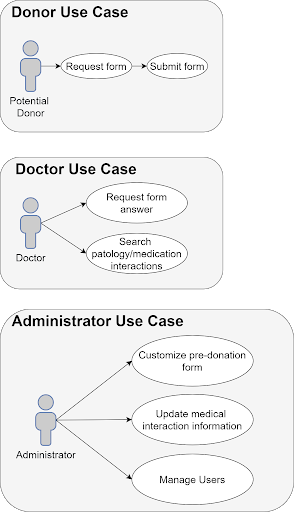
\includegraphics[trim={0 370 70 0},clip]{./figures/useCases.png}}
	\end{center}
	\caption{Donor use case.}\label{fig:donor_use_case}
\end{figure}

After a donor submits their form responses a doctor user will be able to access their answers by searching by the user's unique id as presented in Figure~\ref{fig:doctor_use_case}.

\begin{figure}[H]
	\begin{center}
		\resizebox{100mm}{!}{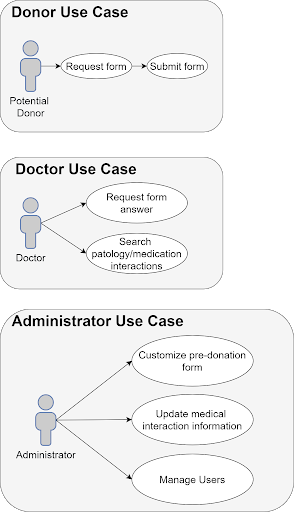
\includegraphics[trim={0 210 70 150},clip]{./figures/useCases.png}}
	\end{center}
	\caption{Doctor use case.}\label{fig:doctor_use_case}
\end{figure}

Furthermore the doctor user is able to search for pathology/medication interactions to resolve any inquiries that might appear during the screening.

Finally the administrator user can update the form structure and flow, update the interaction information and manage the platform's users.
The administrator use case is presented in Figure ~\ref{fig:administrator_use_case}.

\begin{figure}[H]
	\begin{center}
		\resizebox{100mm}{!}{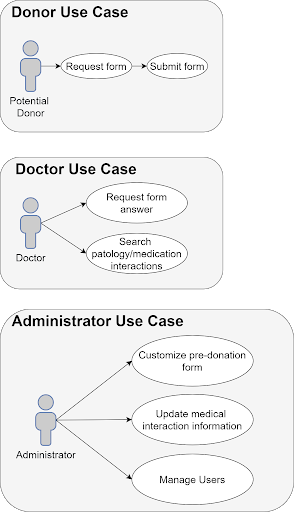
\includegraphics[trim={0 0 0 300},clip]{./figures/useCases.png}}
	\end{center}
	\caption{Administrator use case.}\label{fig:administrator_use_case}
\end{figure}

% Capitulo 3
%
% Capítulo 4
%
\chapter{Architecture} \label{cap:architecture}

This chapter provides an overview of the system’s components and their interactions.
It outlines the capabilities of the project and presents the architecture, entities, and
implementation blueprint that have been designed and developed.

\section{Overview}

Figure ~\ref{fig:architecture} presents a diagram illustrating the main components of the system and their interactions. The system consists of a backend application (server-side) and a frontend application (client-side).
The backend architecture consists of routes, services, and repositories. The routes handle incoming HTTP requests and call the appropriate service. The services manage data manipulation, validation, and interactions with external APIs or databases. Finally, the processed data is sent to the repositories, which store it in the database.

\begin{figure}[H]
	\begin{center}
		\resizebox{160mm}{!}{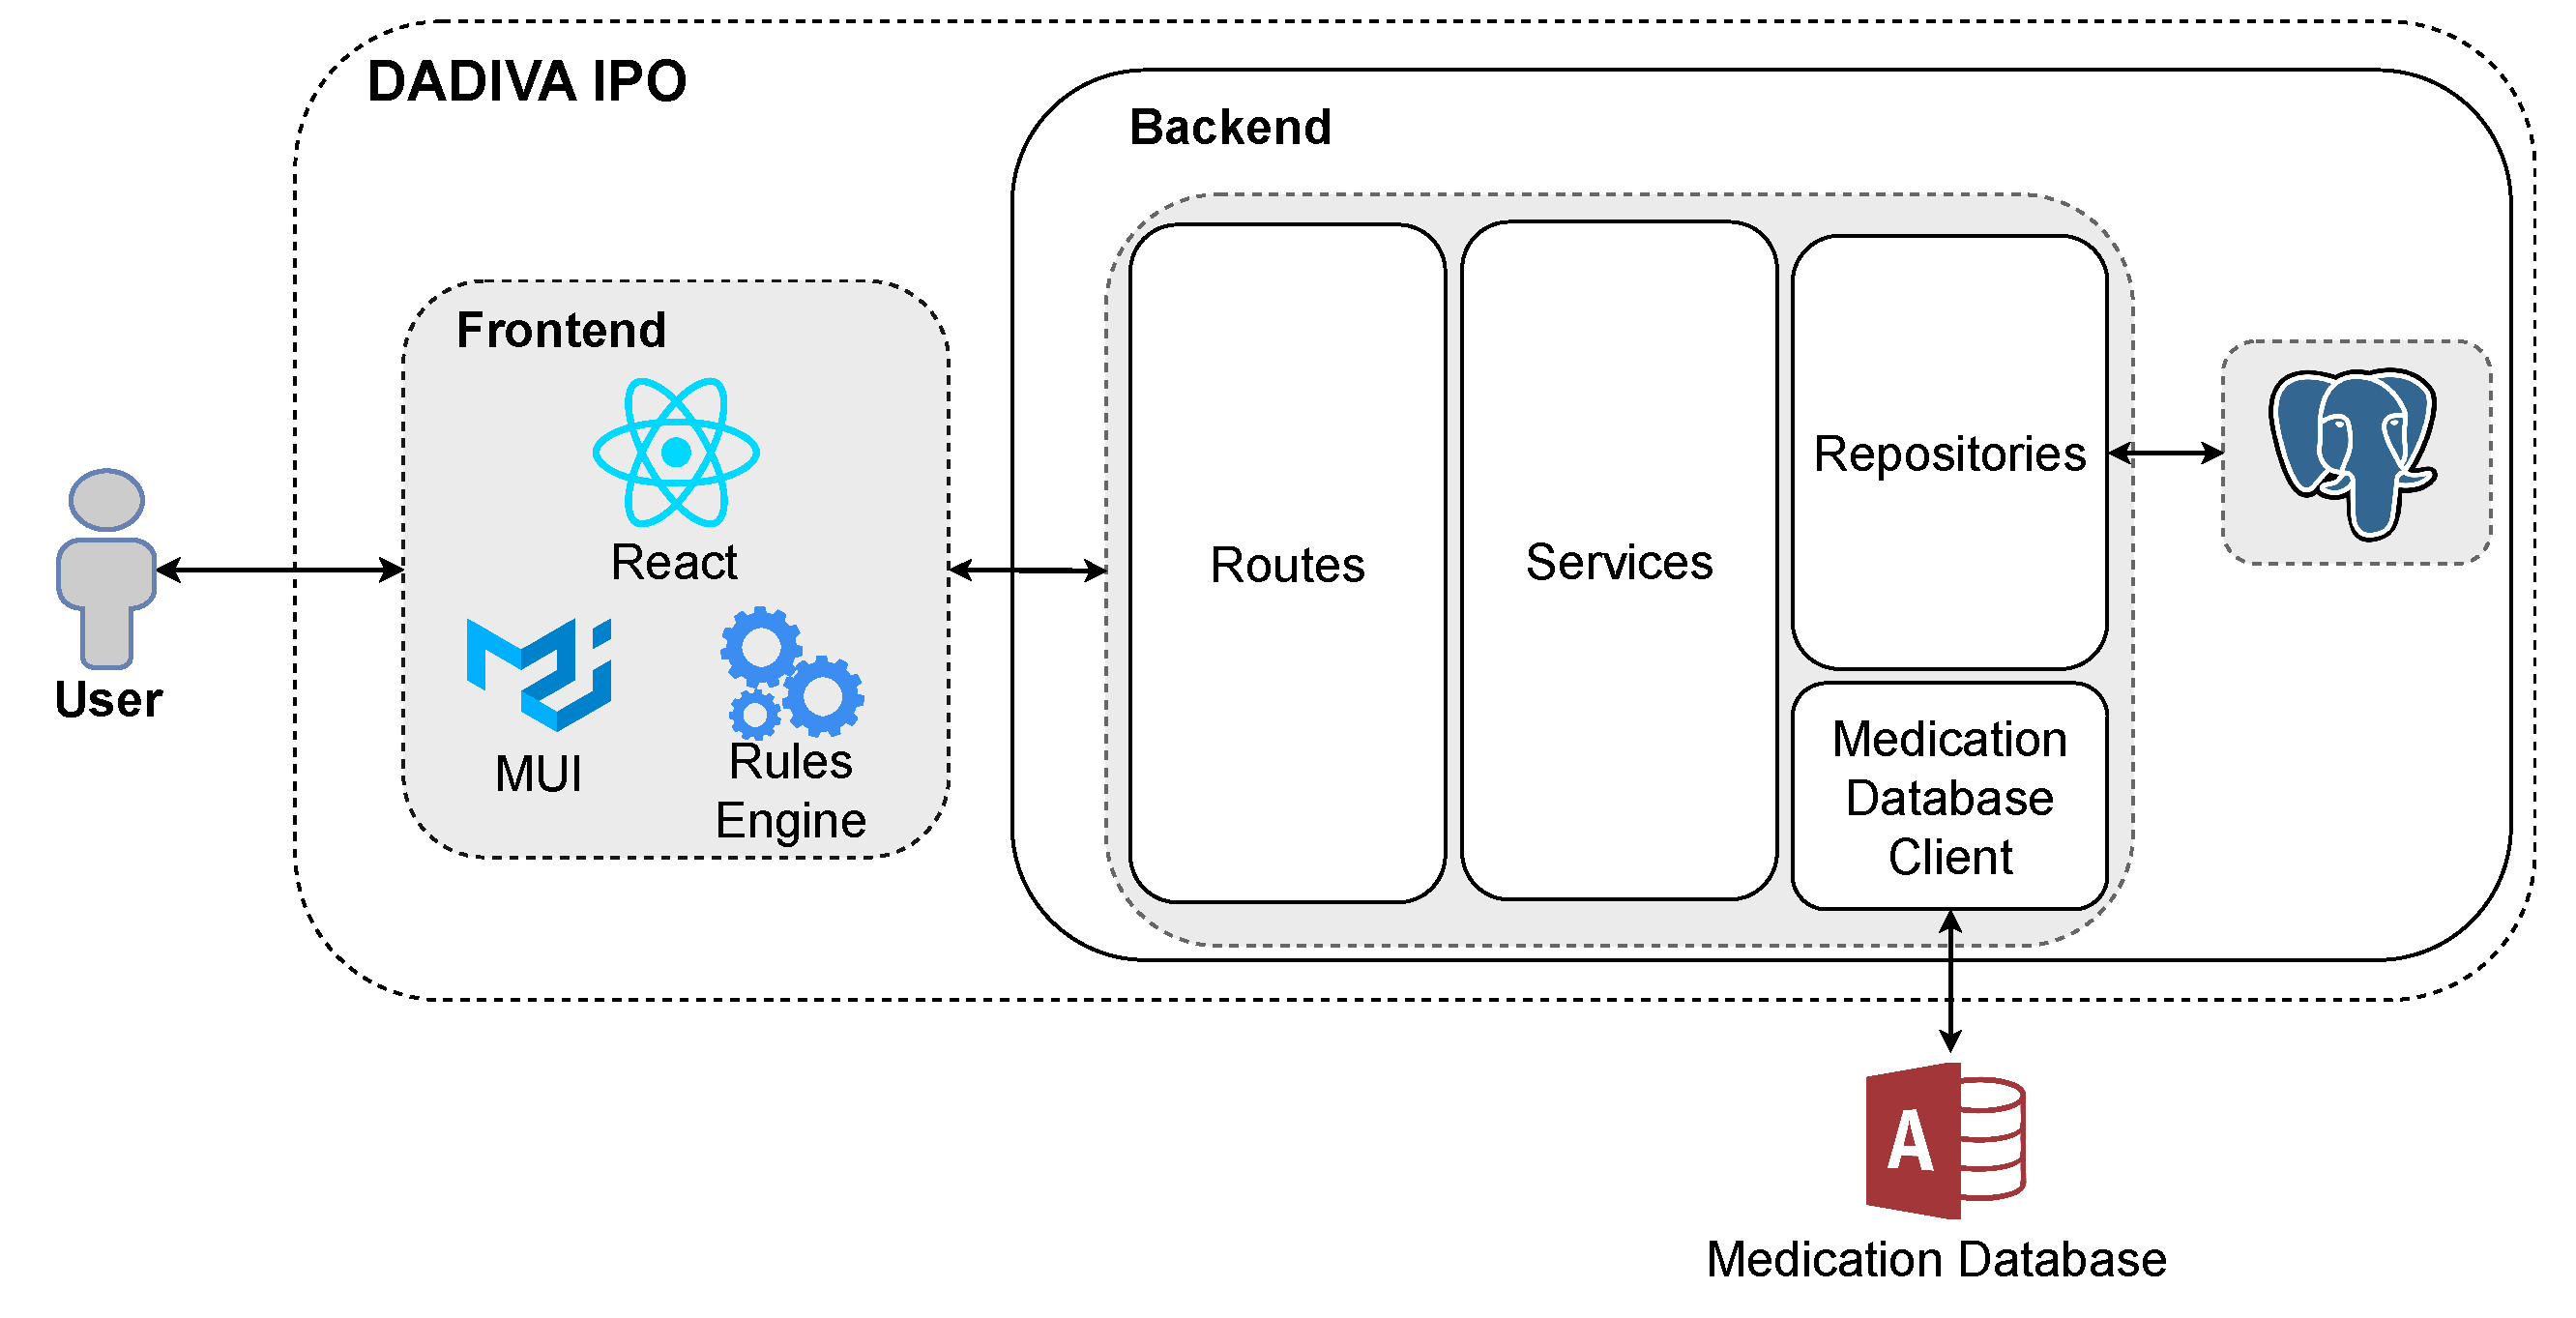
\includegraphics{./figures/Architecture.pdf}}
	\end{center}
	\caption{Application Architecture, gray squares represent containerized components of the solution.}\label{fig:architecture}
\end{figure}

\section{Backend Application}

The backend application can be abstracted into 3 layers:
\begin{itemize}
	\item routes: responsible for receiving the http request and calling the correct service;
	\item services: contains the services that manage the business logic of the application;
	\item repositories: contains the repository layer of the application, uses the ElasticSearchClient;
\end{itemize}


%The backend handles HTTP requests directed to specific endpoints. The route associated with each endpoint converts the request body into an appropriate model, if necessary, and then calls the corresponding service, passing along the model. The service validates the model, converts it into a domain object, and calls the relevant repository. Using an ElasticClient, the repository stores the object in the ElasticSearch database. The appropriate response is then propagated back up, as illustrated in Figure ~\ref{fig:backendLayers}.
%
%\begin{figure}[H]
%	\begin{center}
%		\resizebox{100mm}{!}{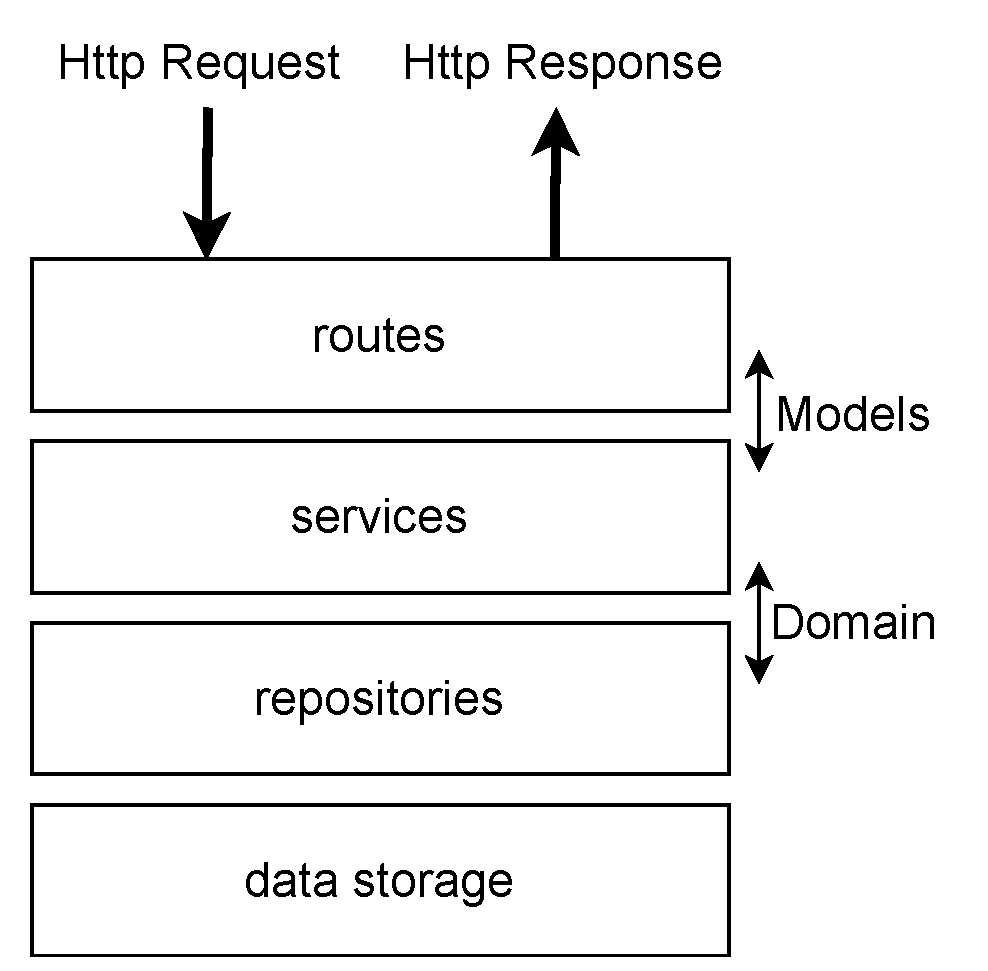
\includegraphics{./figures/backendLayers.pdf}}
%	\end{center}
%	\caption{Backend layers.}\label{fig:backendLayers}
%\end{figure}

The service layer is composed by the following elements:

\begin{itemize}
	\item form: responsible for form management, such as, creation, requests, submission, editing and deletion;
	\item search: responsible for medication and pathology interaction information retrieval;
	\item users: responsible for user management, such as, registration, login, deletion and role management.
\end{itemize}

The repositories communicate with the database, in which the various data models are divided into specific indexes, such as:

\begin{itemize}
	\item /form: stores all the form structures;
	\item /submissions: stores all the user form responses;
	\item /inconsistencies: stores all the user form inconsistencies;
	\item /users: stores all the users.
\end{itemize}

An example of a GET request for the form resource is presented in Figure ~\ref{fig:getForm_Sequence_Diagram}

\begin{figure}[H]
	\begin{center}
		\resizebox{160mm}{!}{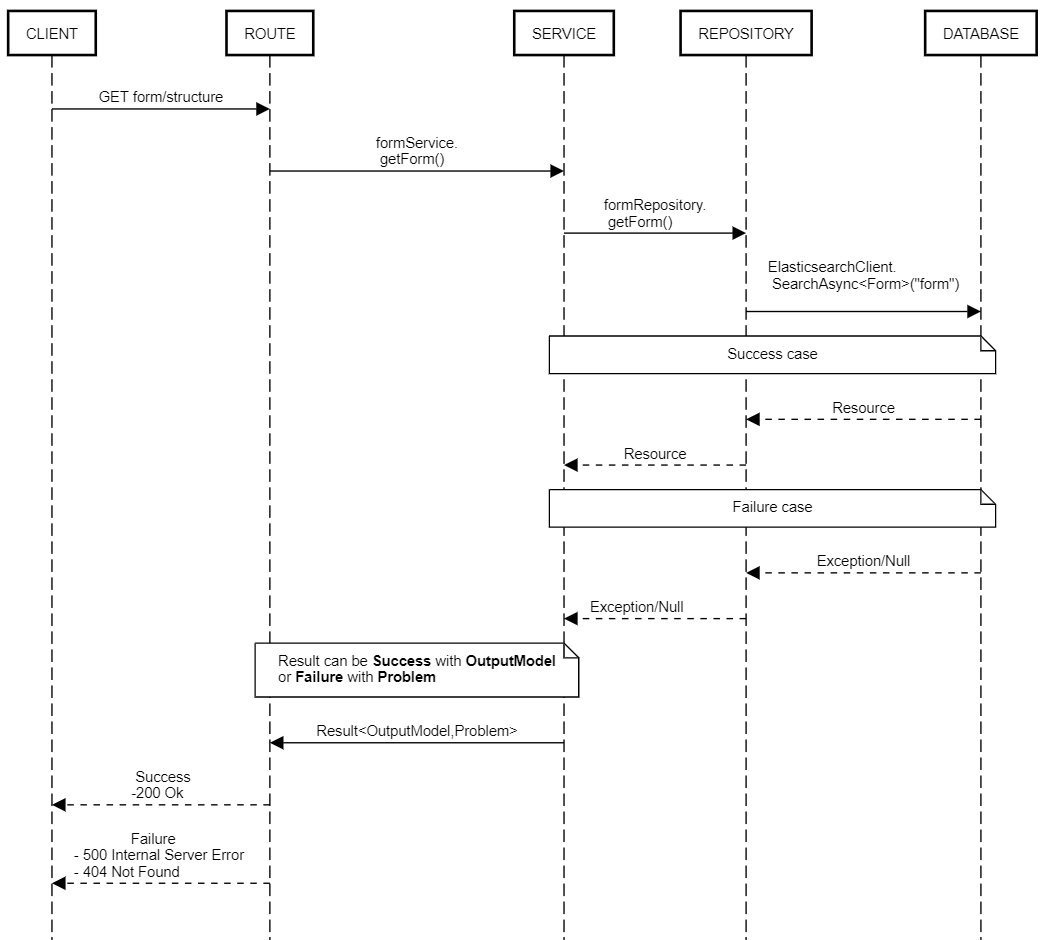
\includegraphics{./figures/getForm_Sequence_Diagram.png}}
	\end{center}
	\caption{Get Form Sequence Diagram.}\label{fig:getForm_Sequence_Diagram}
\end{figure}


\section{Form Data Model and Inconsistencies Data Model}

The first approach to solve the dynamic form challenge was to use a data structure formed by pairs of main questions and sub-questions, example presented in Figure ~\ref{fig:old_form}, where a main question can only be answered with boolean values, and one of those values triggers the display of a sub-question which has a certain type of response, such as boolean, dropdown for known multiple answers, and text, to accept user text input.

\begin{figure}[hbt!]
	\begin{center}
		\resizebox{150mm}{!}{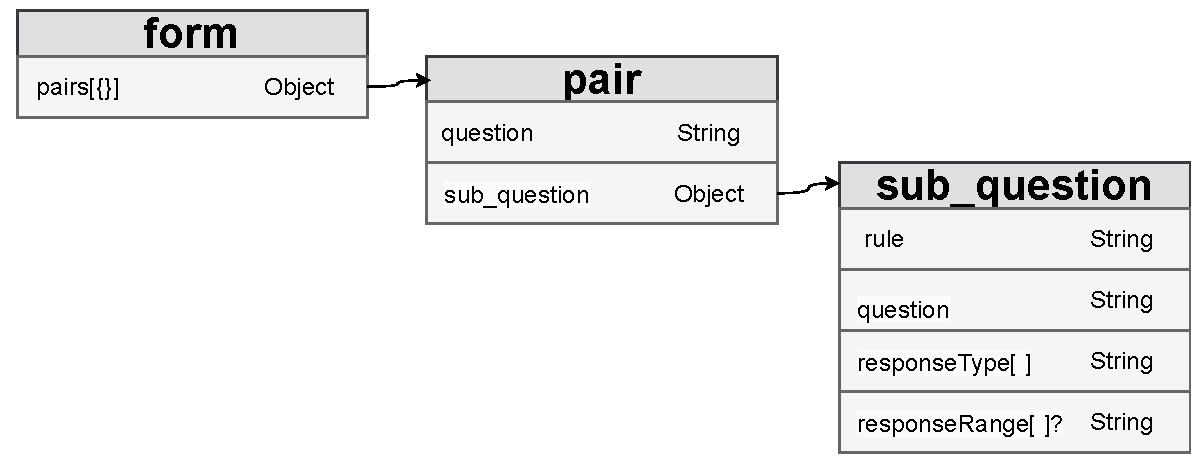
\includegraphics{./figures/oldForm.pdf}}
	\end{center}
	\caption{First Form Data Structure.}\label{fig:old_form}
\end{figure}

This approach has several drawbacks. Firstly, it prevents the suppression of further questions, which contradicts the goal of creating a flexible and adaptable solution. Additionally, it conflates questions and rules within sub-questions, leading to a lack of clarity and potential confusion in implementation.

Upon further discussion we settled on using a more complex data structure , exemplified in Figure ~\ref{fig:new_form}, composed by a list of questions and a list of rules.

Each question has an id, the text that composes it, the type of response (boolean, text and dropdown) and can have options that lists all the possibles values for a multiple(dropdown) response.

Each rule has conditions, which can be "any","all" or "not", so that, when any, all or none of the conditions are met an event is triggered.
Each condition type will have a fact, an operator and a value. In essence, when a question, which is identified by the fact field via it's id, is answered a condition can true or false depending on the logical operator used, ie equal or notEqual, and the value of the answer. If the condition is true an event is triggered, this event can be to show or hide a subsequent question, this targeted question is identified via the id, supplied in the params field.

This model, specifically the rules field, was chosen as it is part of the JSON-Rules-Engine specification, which is presented in more detail in Chapter ~\ref{cap:technologies} and is easily stored and retrieved in a ElasticSearch database.

\begin{figure}[htbp]
	\begin{center}
		{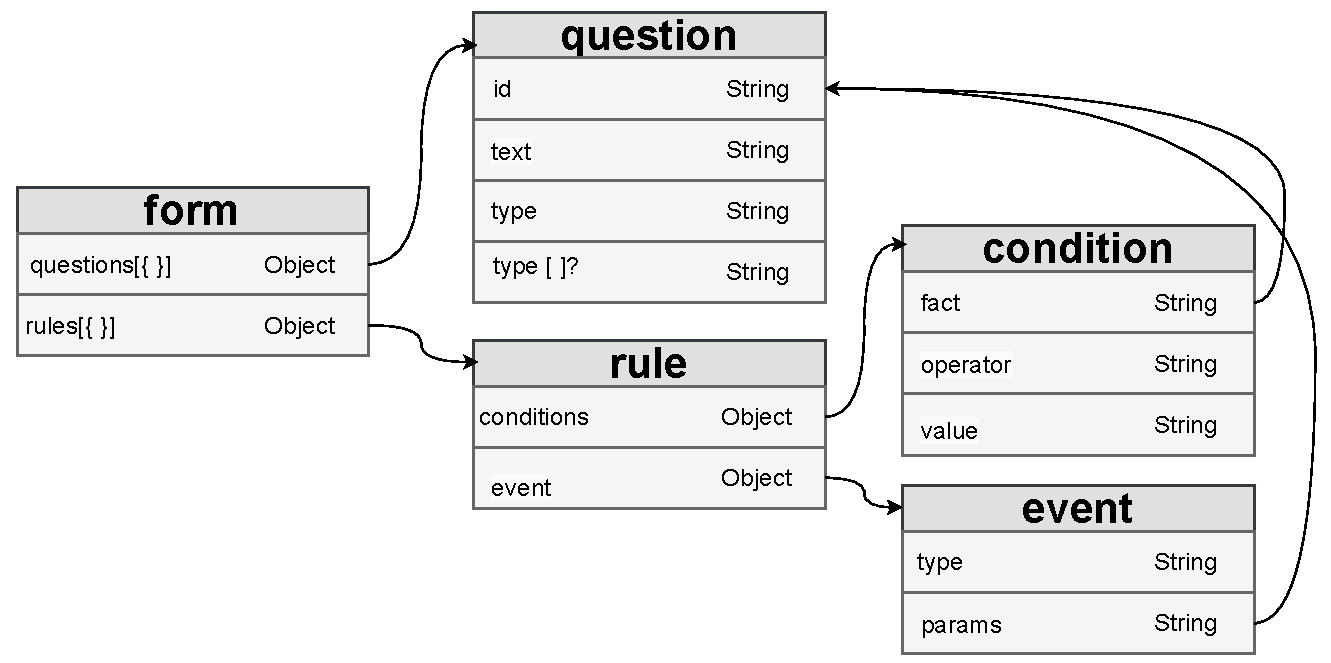
\includegraphics[width=\textwidth,height=\textheight,keepaspectratio]{./figures/newForm.pdf}}
	\end{center}
	\caption{Final Form Data Structure.}\label{fig:new_form}
\end{figure}
\FloatBarrier

The inconsistencies data model is compromised of rules, and describes answer combinations that are logical fallacies, ie a donor answering that they're healthy in one question and that they have a chronic disease in another question.

\section{Submission Data Model}

The submission data structure represents and answered form, has such it contains a list of answered questions, each answered question is composed by the question id and the answer, as referenced in Figure ~\ref{fig:submission_data_model}.

\begin{figure}[hbt!]
	\begin{center}
		\resizebox{150mm}{!}{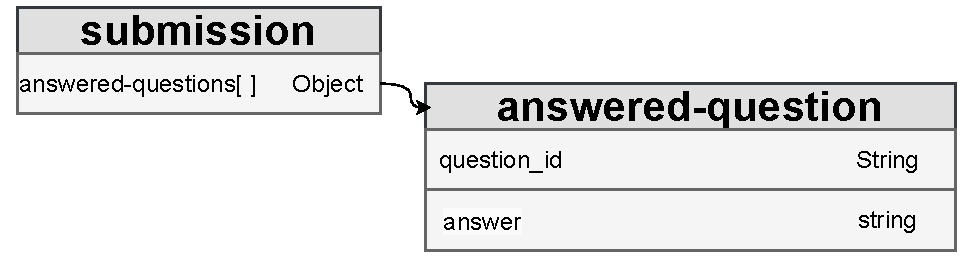
\includegraphics{./figures/Submission_Data_Model.pdf}}
	\end{center}
	\caption{Submission Data Structure.}\label{fig:submission_data_model}
\end{figure}


\section{User Data Model}

The user data structure is composed on an unique identifier, the nic, and the user hashed password, as referenced in Figure ~\ref{fig:user_data_model}.

\begin{figure}[hbt!]
	\begin{center}
		\resizebox{150mm}{!}{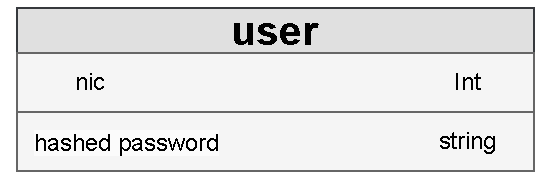
\includegraphics{./figures/User_Data_Structure.pdf}}
	\end{center}
	\caption{User Data Structure.}\label{fig:user_data_model}
\end{figure}

%%secalhar é mais adequado na descrição do problema
\section{IPO Medication Portal}
\textcolor{red}{
The IPST medication guideline are organized in a table like manner, in the following column layout:
	\begin{enumerate}
		\item Class/Group of Medication: This column categorizes medications.
		\item Active Substance/Commercial Name: This column lists either the active ingredient or the brand name of the medication.
		\item Criteria: This column specifies if a particular class or group of medications affects eligibility for blood donation, including details such as the duration of ineligibility and other relevant conditions.
	\end{enumerate}
	The terms used in the first column are, from what we can access, similar to the available pharmacotherapeutic classifications. A reliable source of a drug's pharmacotherapeutic classification is a portal provided by Infarmed to it's partner organizations, such as Lisbon's IPO.
	As such, upon a donor's form submission, assuming they where taking some medication, our application would perform requests to said portal, get the appropriate pharmacotherapeutic classification and, by cross-checking the classification with the term used in the first column of the guidelines, return the relevant information.
	However the terms used in the guidelines don't always reflect the available classifications, and, as such, the platform will employ a dictionary that associates the terms used in the guidelines to pharmacotherapeutic classifications. This dictionary will be updatable by the platform's administrators.
	The fact that the IPST guidelines aren't available in a machine readable format persists.
}

\section{Frontend Application}\label{architecture_frontend}

The frontend application is a web-based interface designed to facilitate seamless interaction between users and the backend system. It features a user-friendly and intuitive interface, catering to different types of users with specific functionalities:

\begin{itemize}
	\item Donor Users: Can fill out the current donation form;
	\item Doctor Users: Can search for pathology and medication interactions with blood donation and request form answers for specific users;
	\item Administrator Users: Can customize the current form, update pathology and medication interaction information, and manage users.
\end{itemize}

The application is organized into multiple pages and components, each serving distinct purposes. It includes a service layer responsible for communicating with the backend application through the REST API.

During planning some mockups where created of the final result for some pages, the login page is presented in Figure ~\ref{fig:login}, the form pages are presented in Figures ~\ref{fig:form},~\ref{fig:form_no} and ~\ref{fig:form_yes}, the backoffice page is presented in Figure ~\ref{fig:backoffice}.

\begin{figure}[H]
	\begin{center}
		\resizebox{160mm}{!}{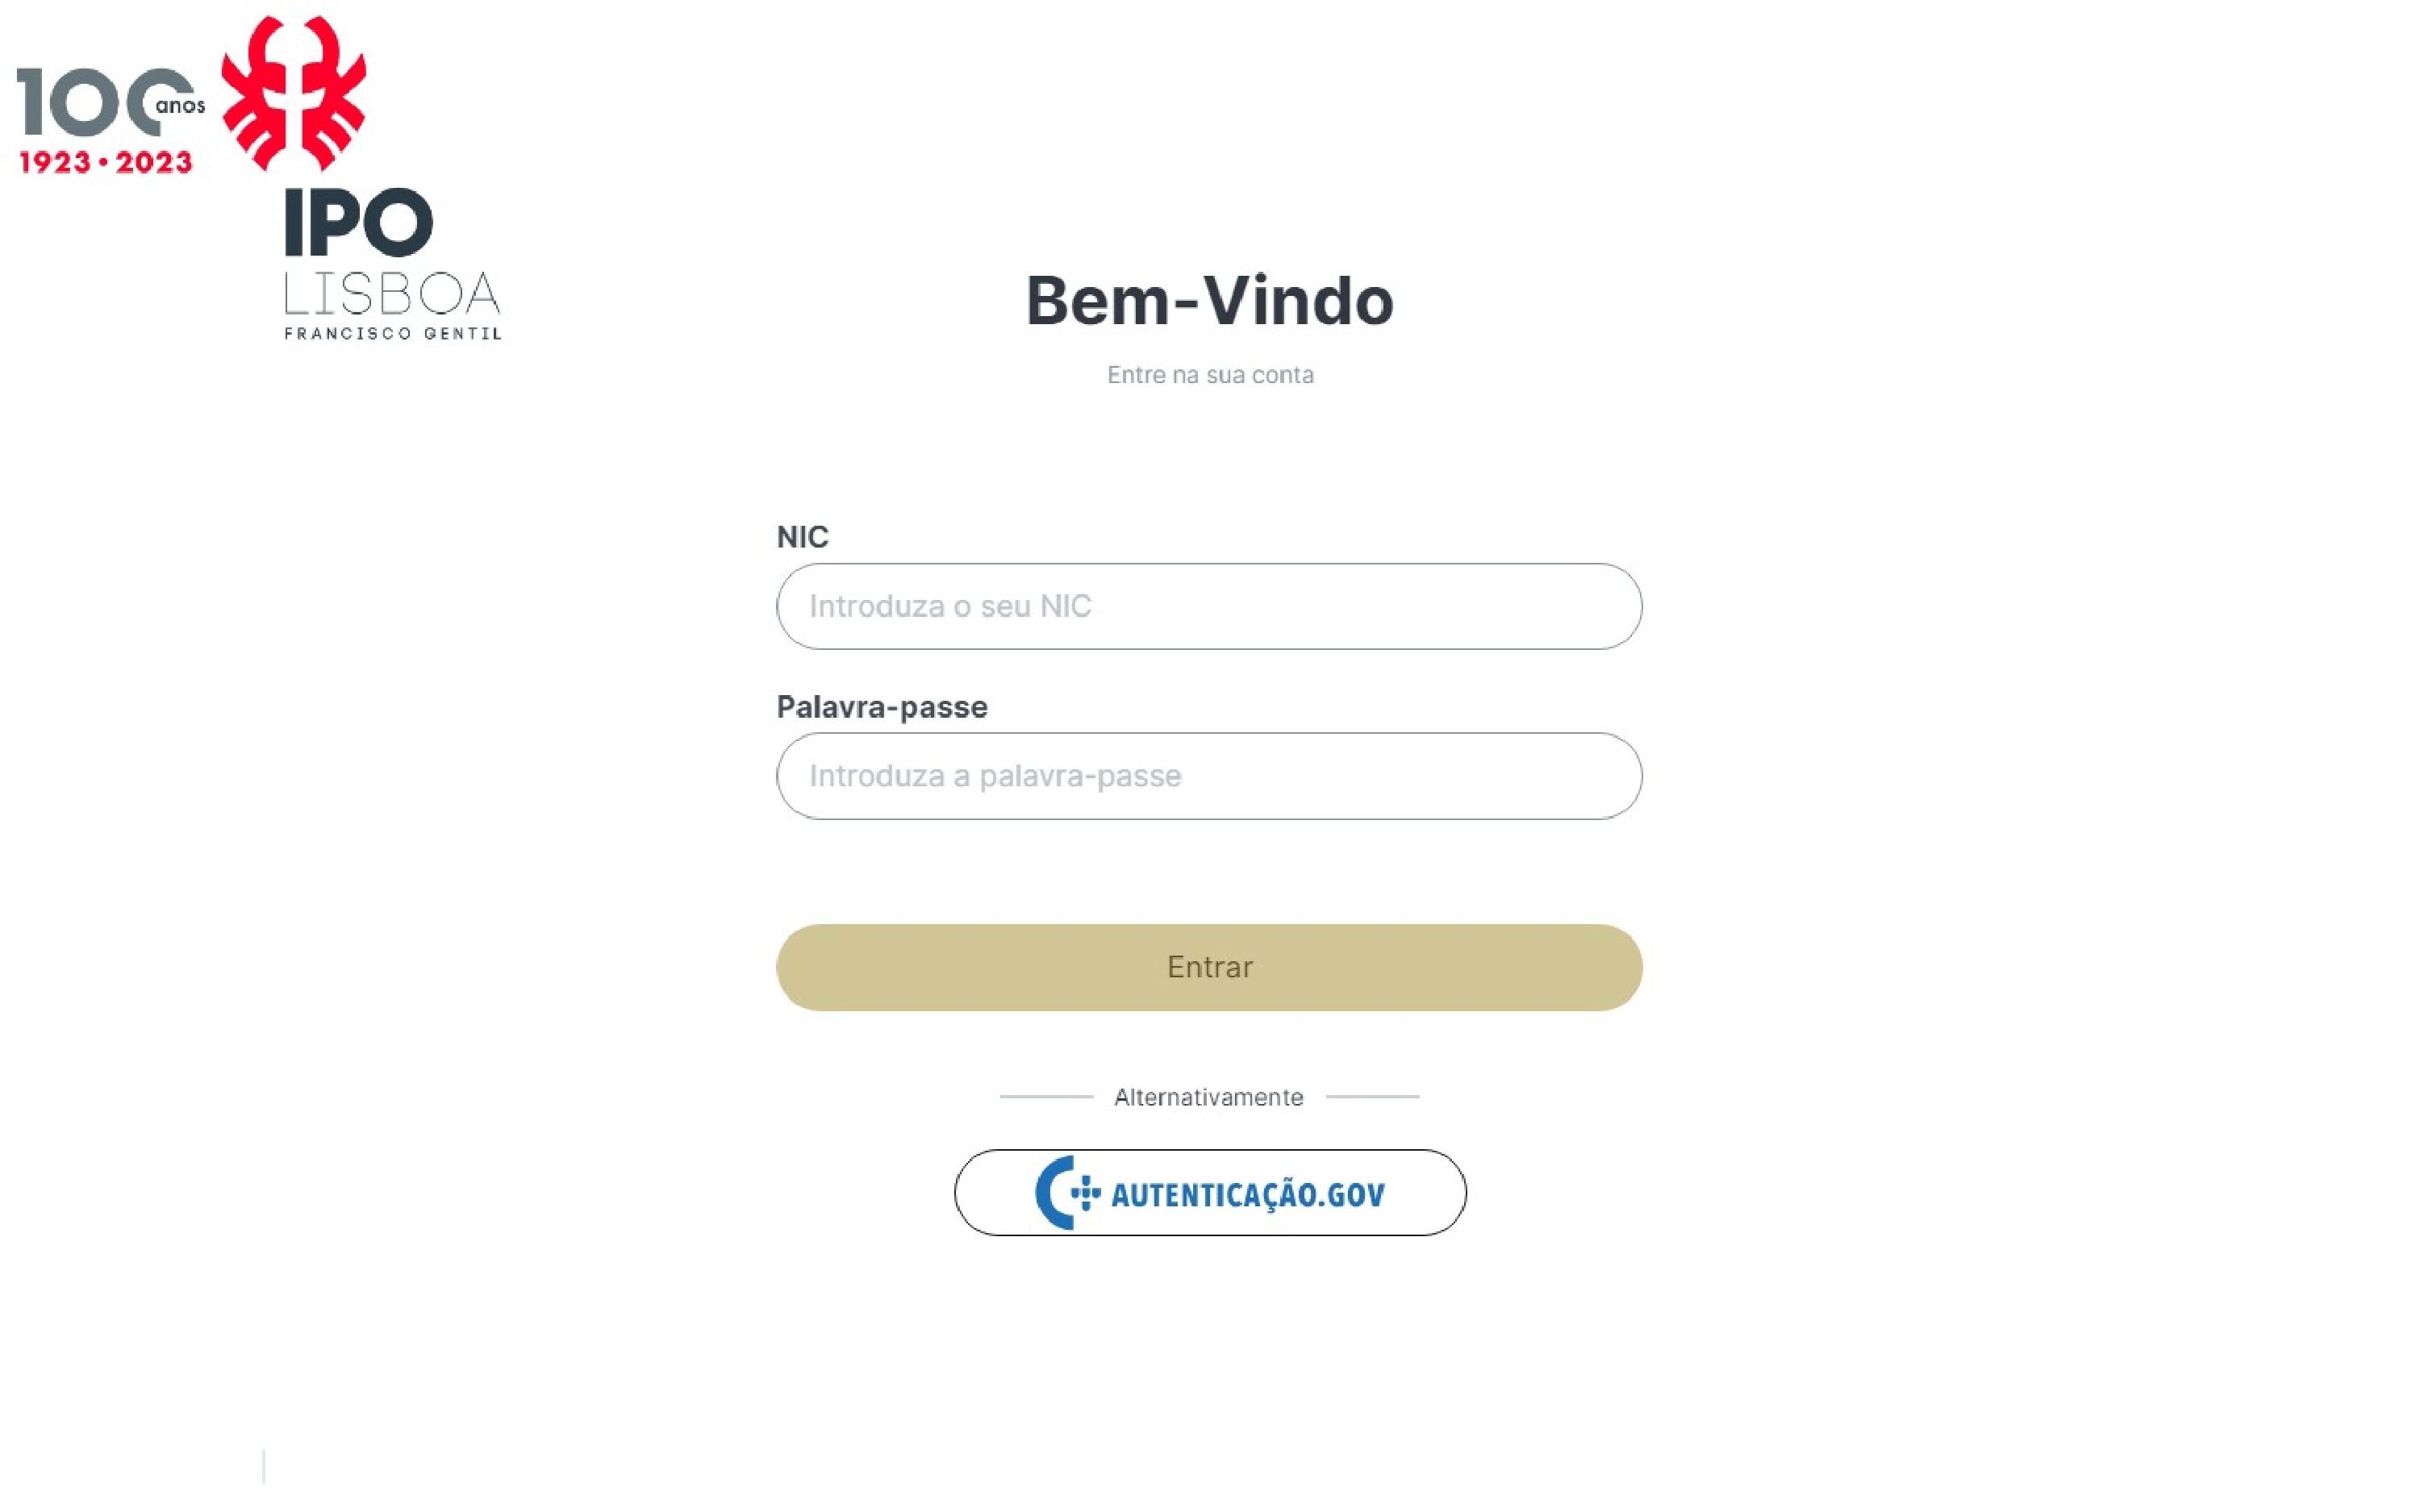
\includegraphics{./figures/Login.pdf}}
	\end{center}
	\caption{Login Page Mock.}\label{fig:login}
\end{figure}

\begin{figure}[H]
	\begin{center}
		\resizebox{160mm}{!}{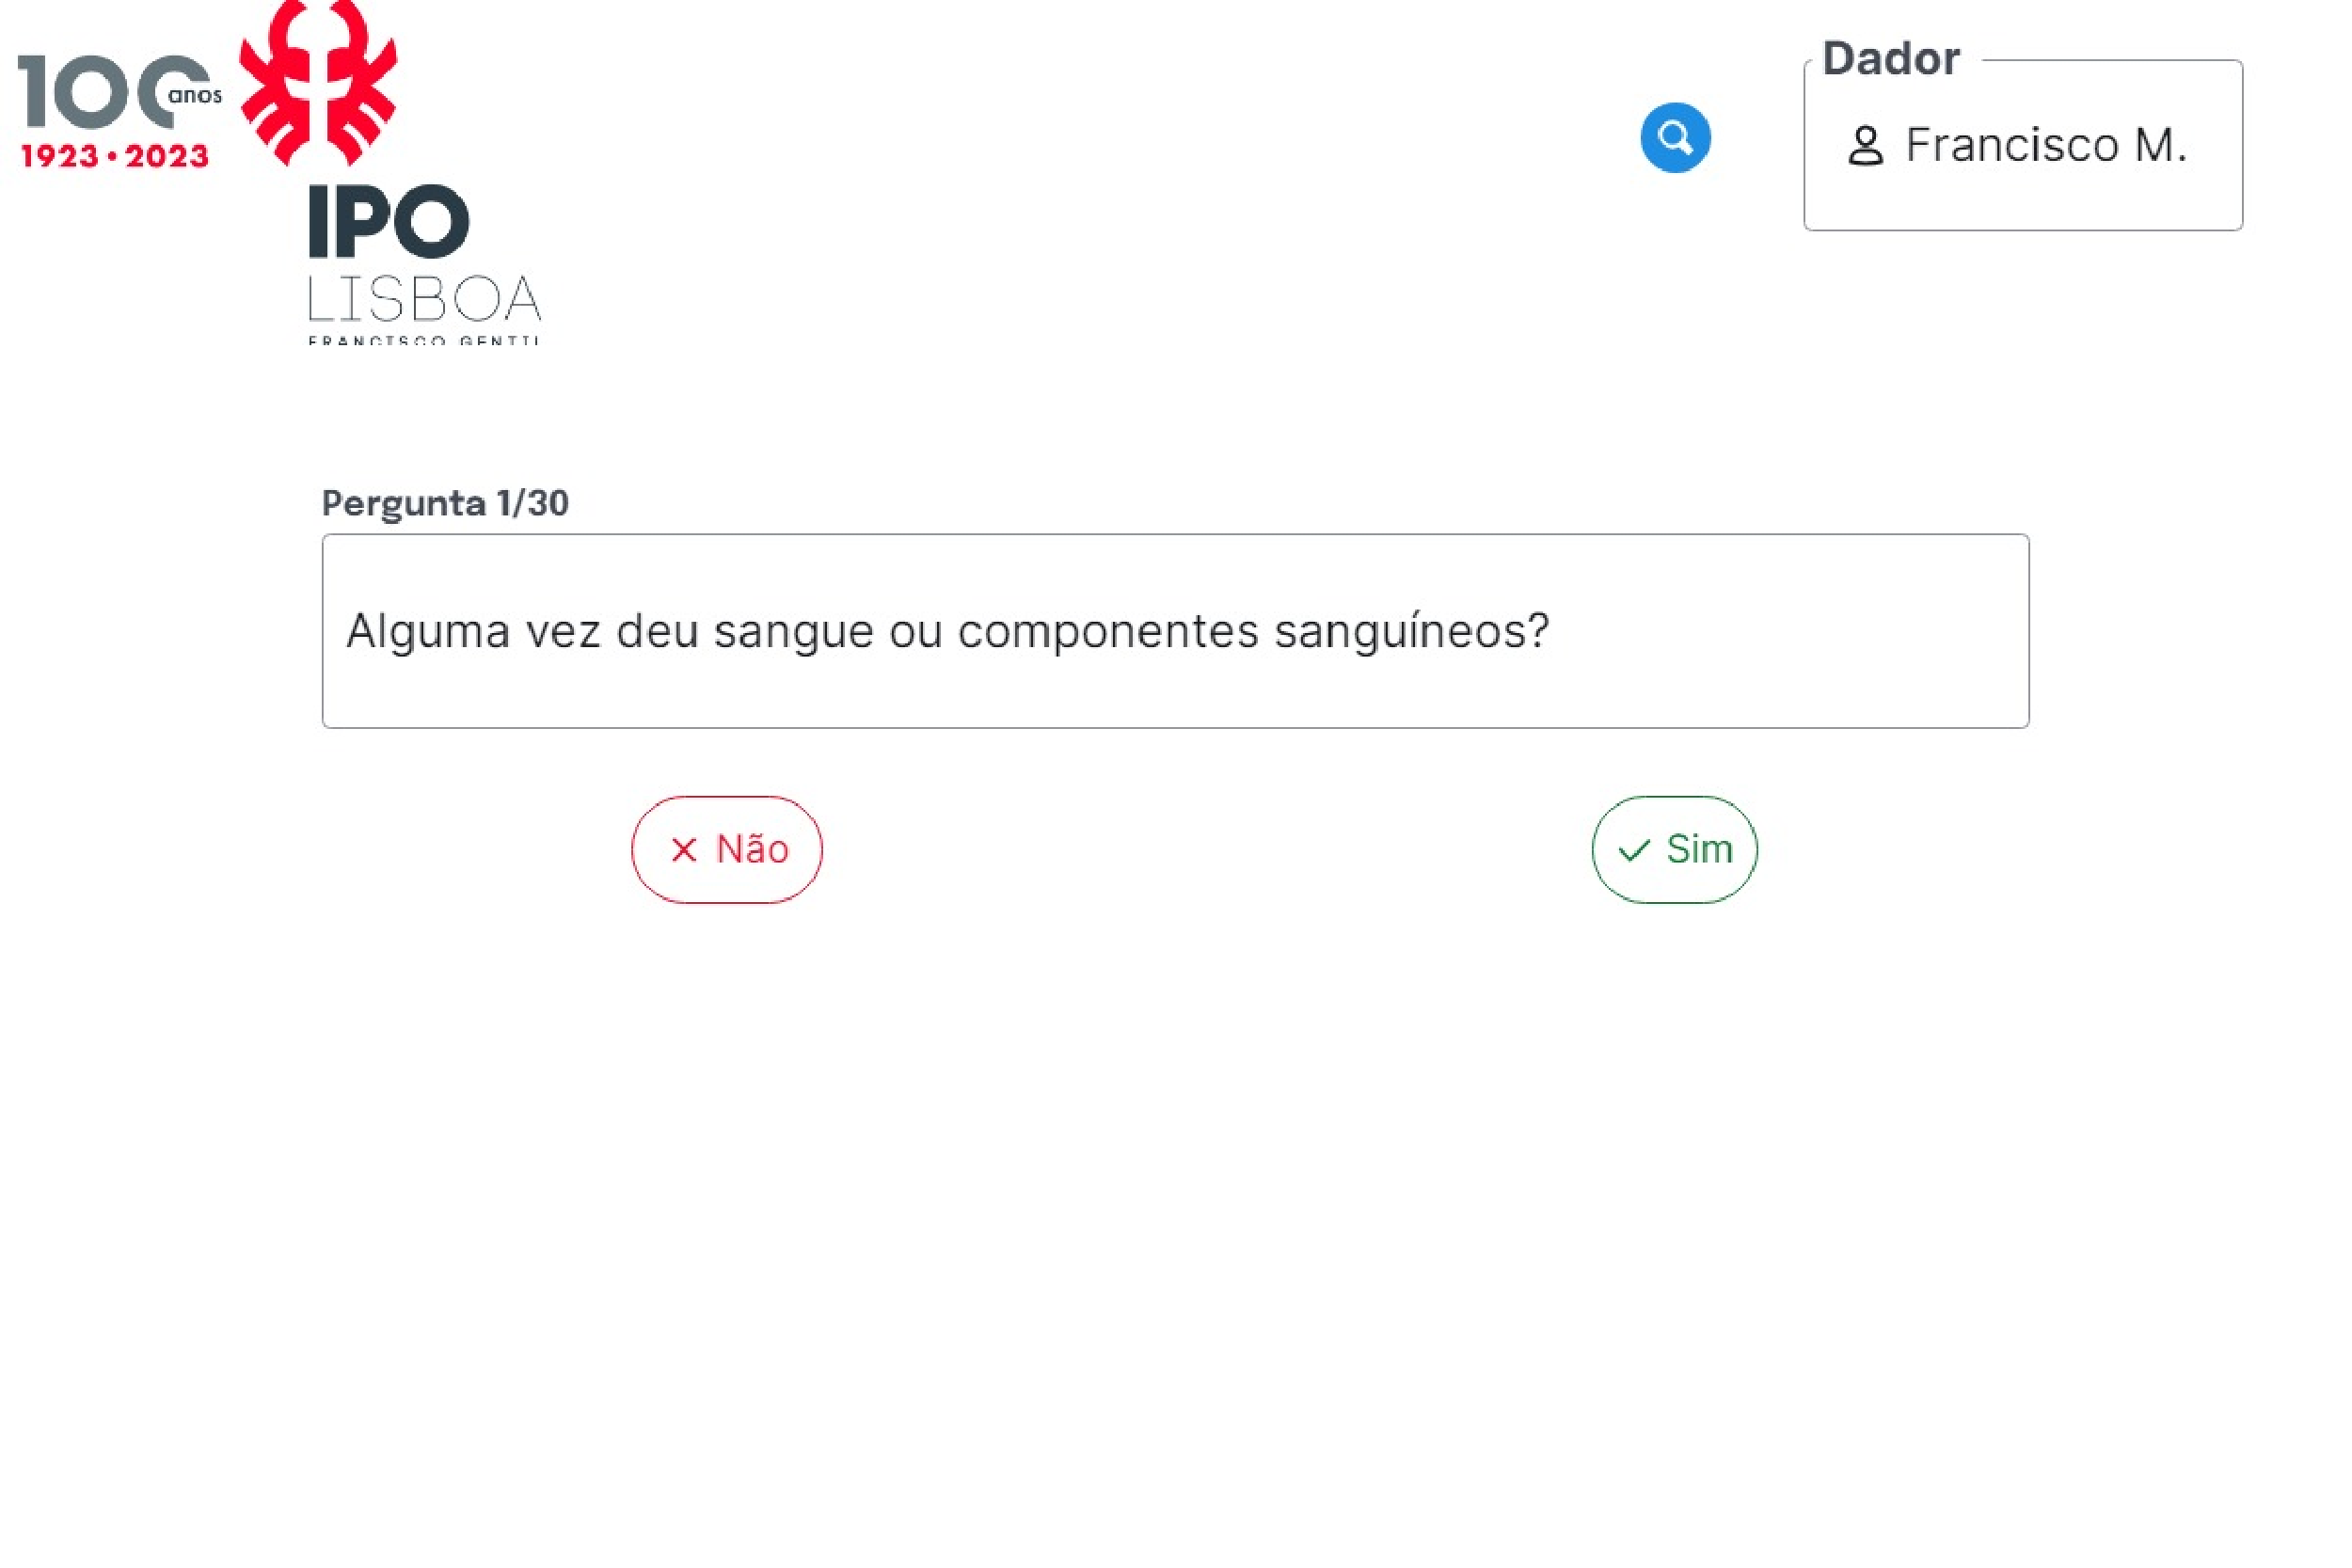
\includegraphics{./figures/Form.pdf}}
	\end{center}
	\caption{Form Page Mock.}\label{fig:form}
\end{figure}

\begin{figure}[H]
	\begin{center}
		\resizebox{160mm}{!}{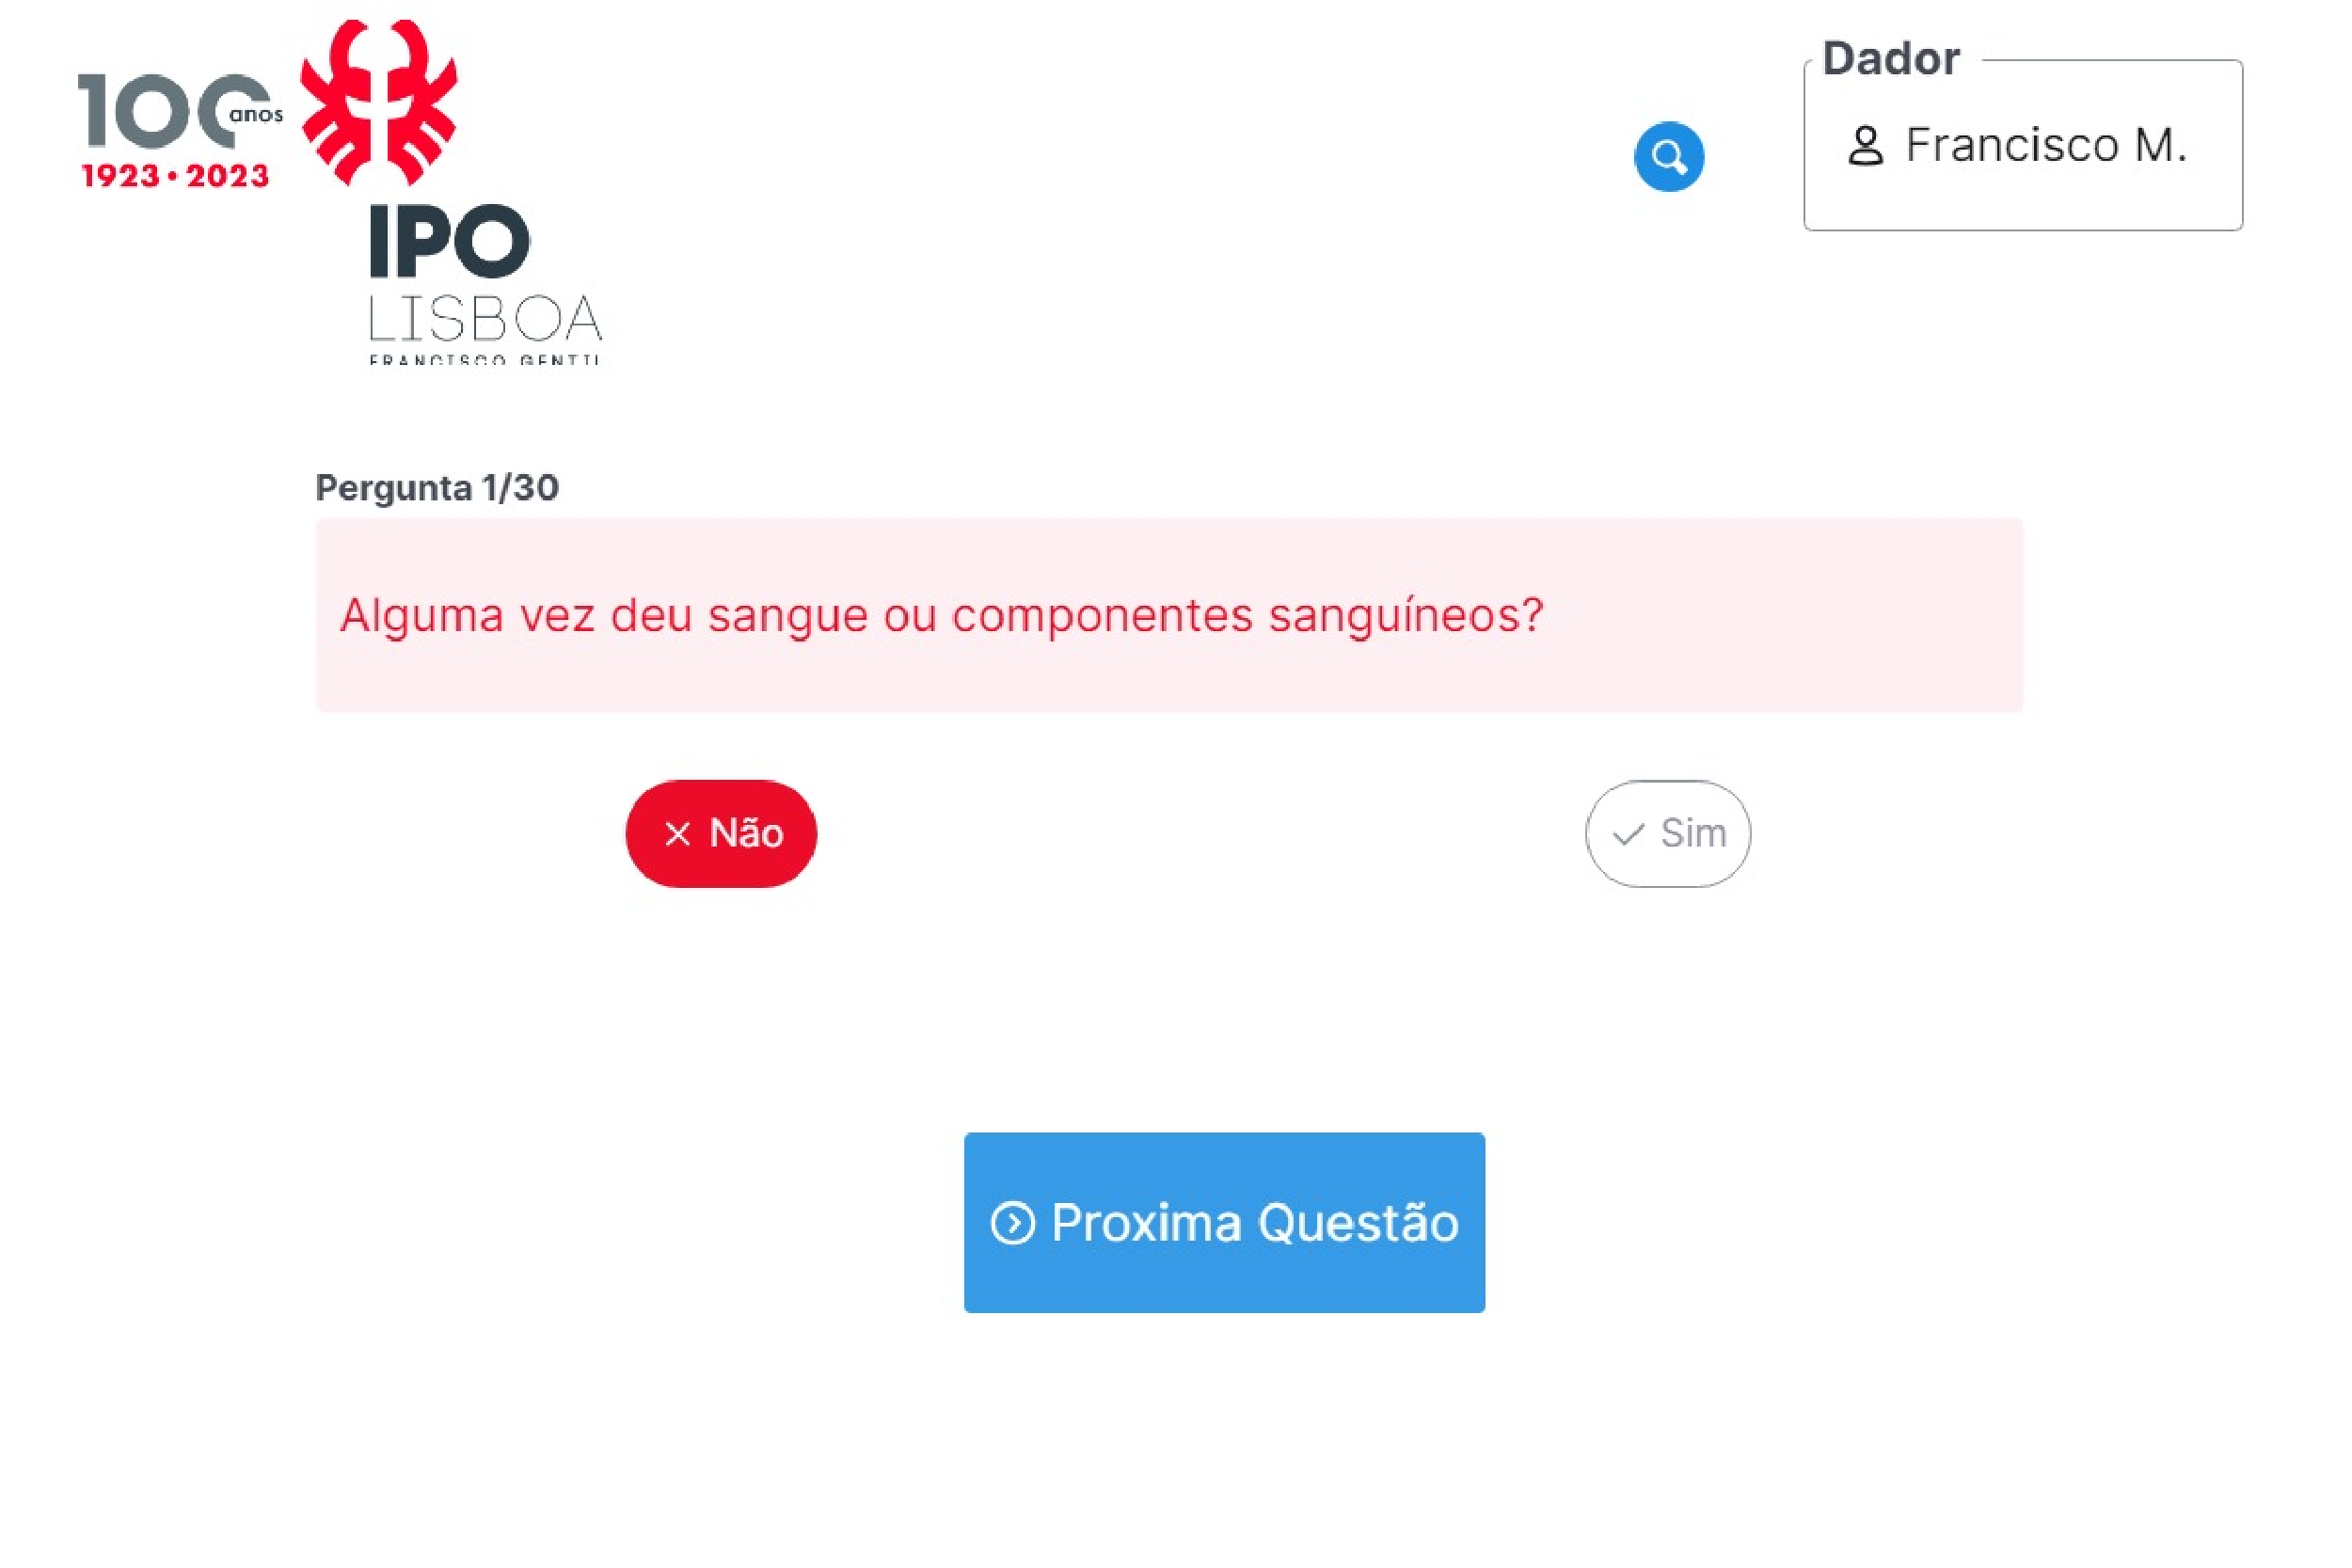
\includegraphics{./figures/Form_Answer_No.pdf}}
	\end{center}
	\caption{Form Page Negative Answer Mock.}\label{fig:form_no}
\end{figure}

\begin{figure}[H]
	\begin{center}
		\resizebox{160mm}{!}{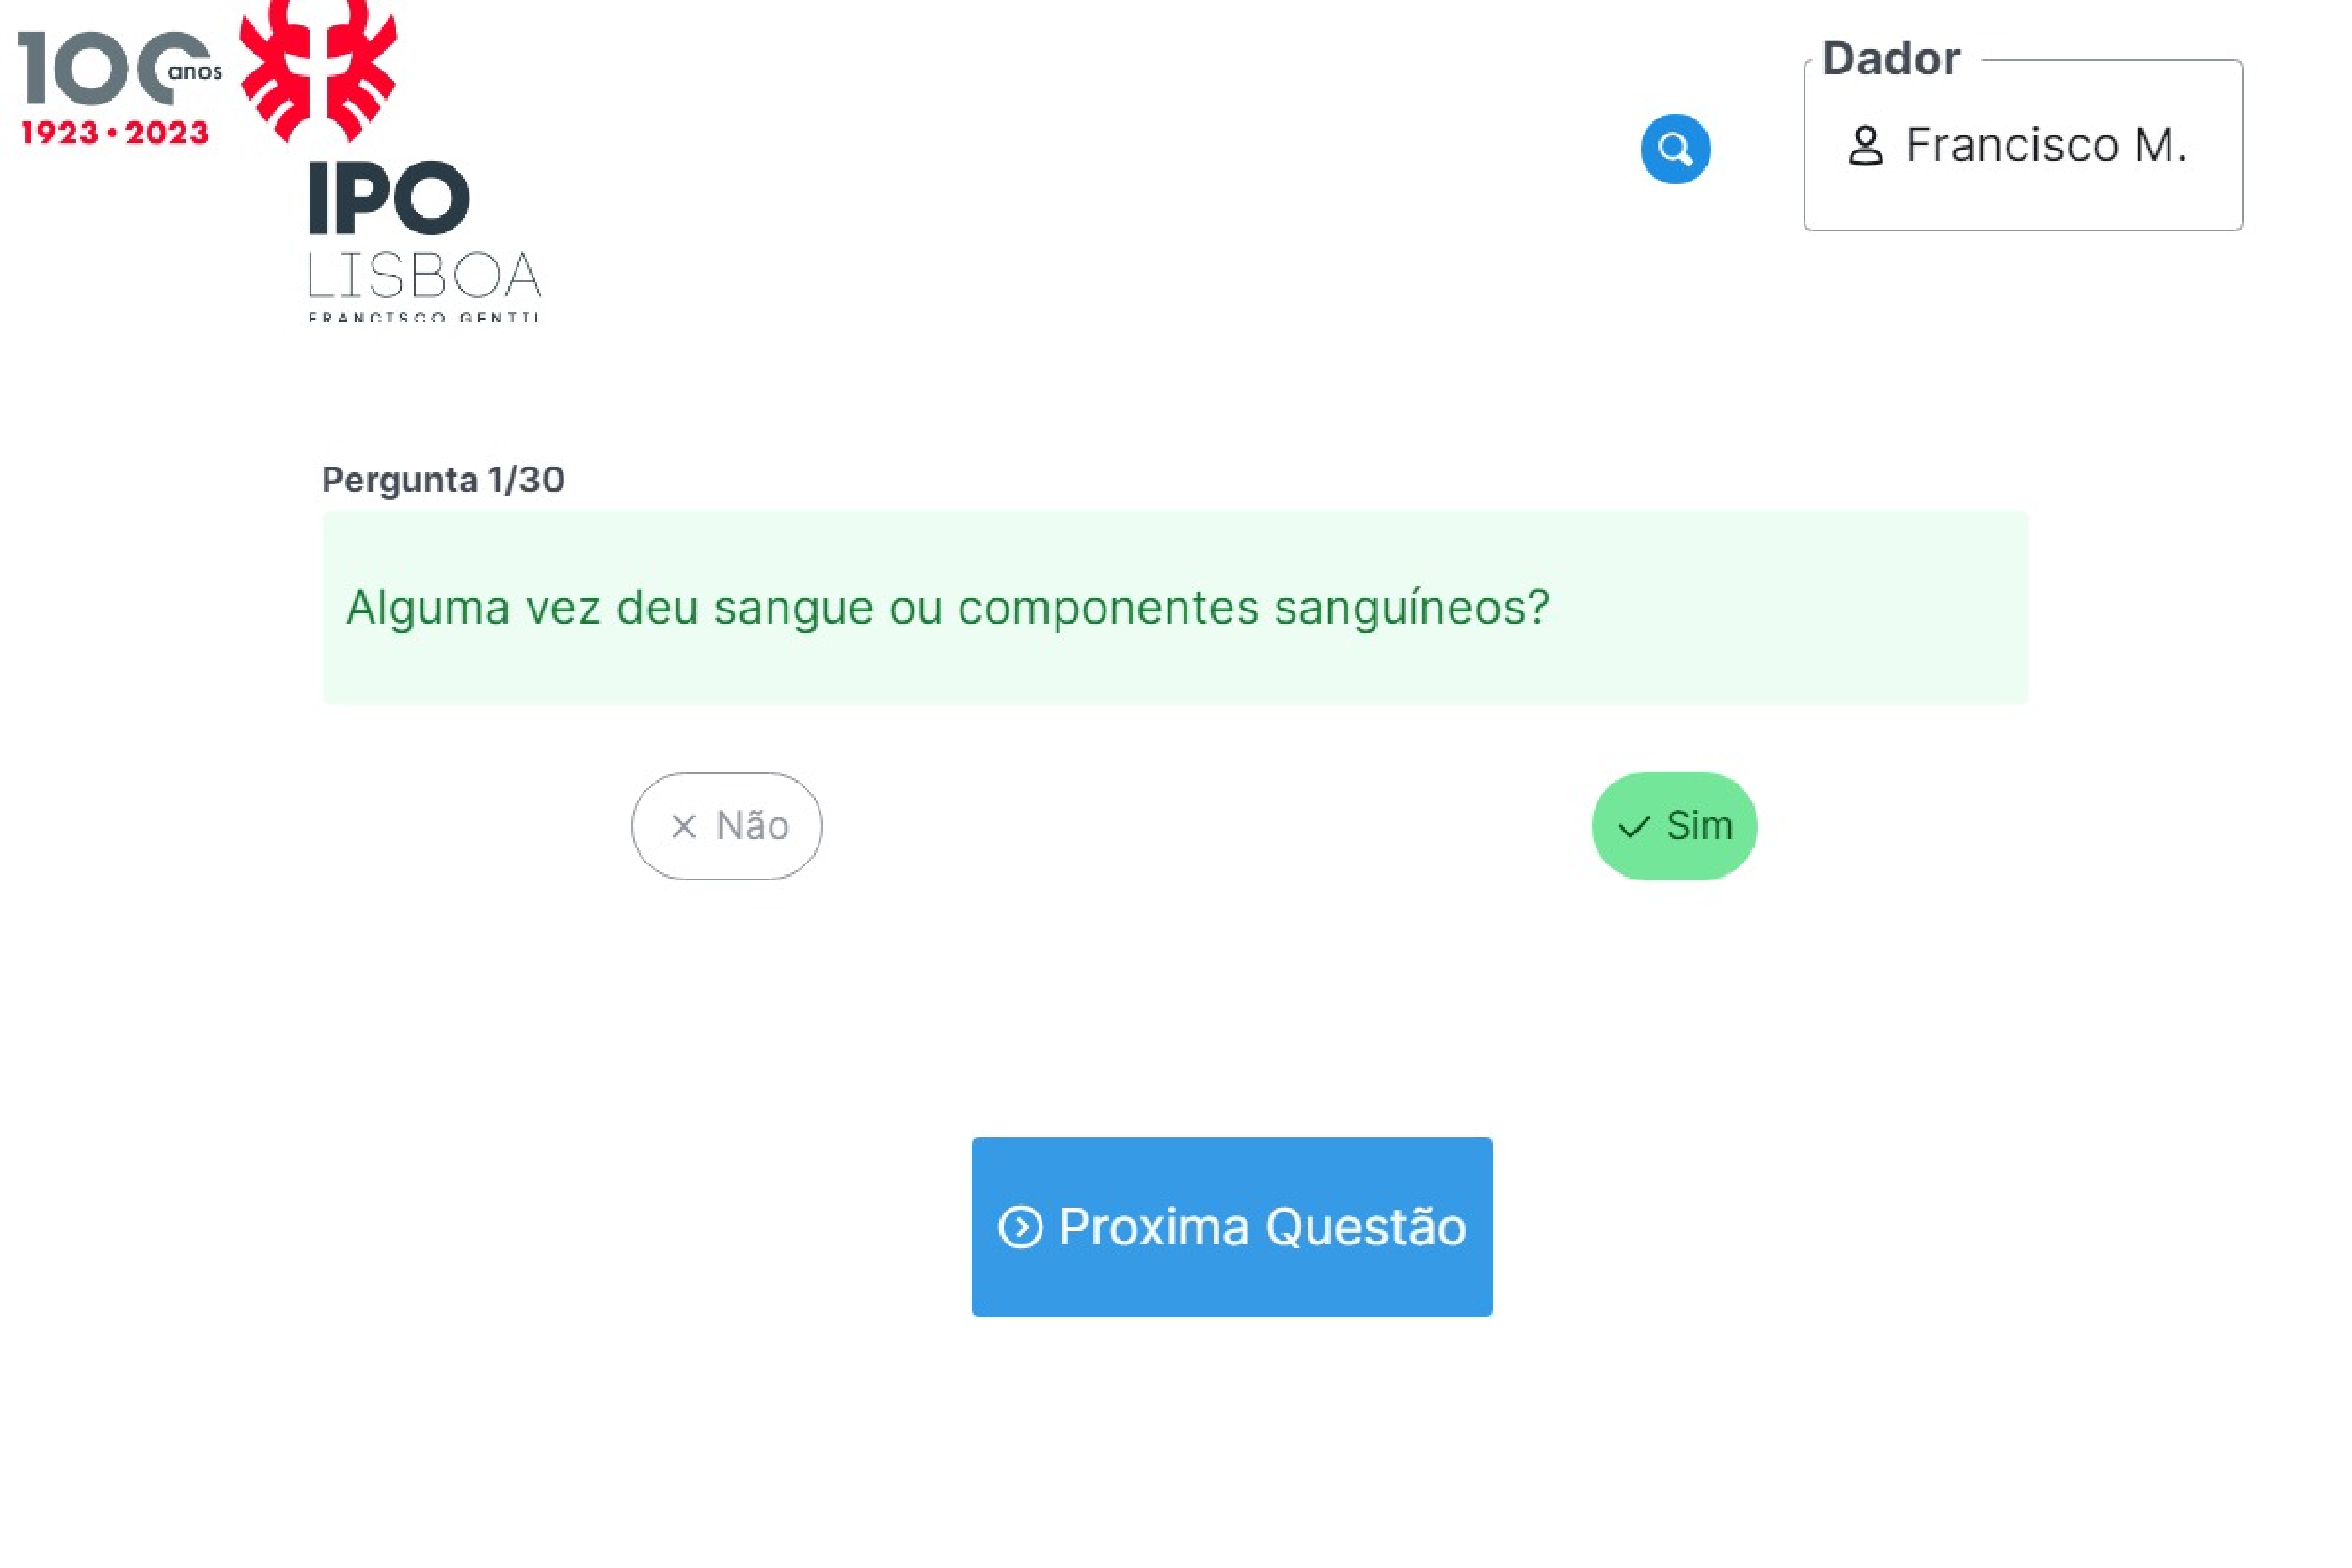
\includegraphics{./figures/Form_Answer_Yes.pdf}}
	\end{center}
	\caption{Form Page Positive Answer Mock.}\label{fig:form_yes}
\end{figure}

\begin{figure}[H]
	\begin{center}
		\resizebox{160mm}{!}{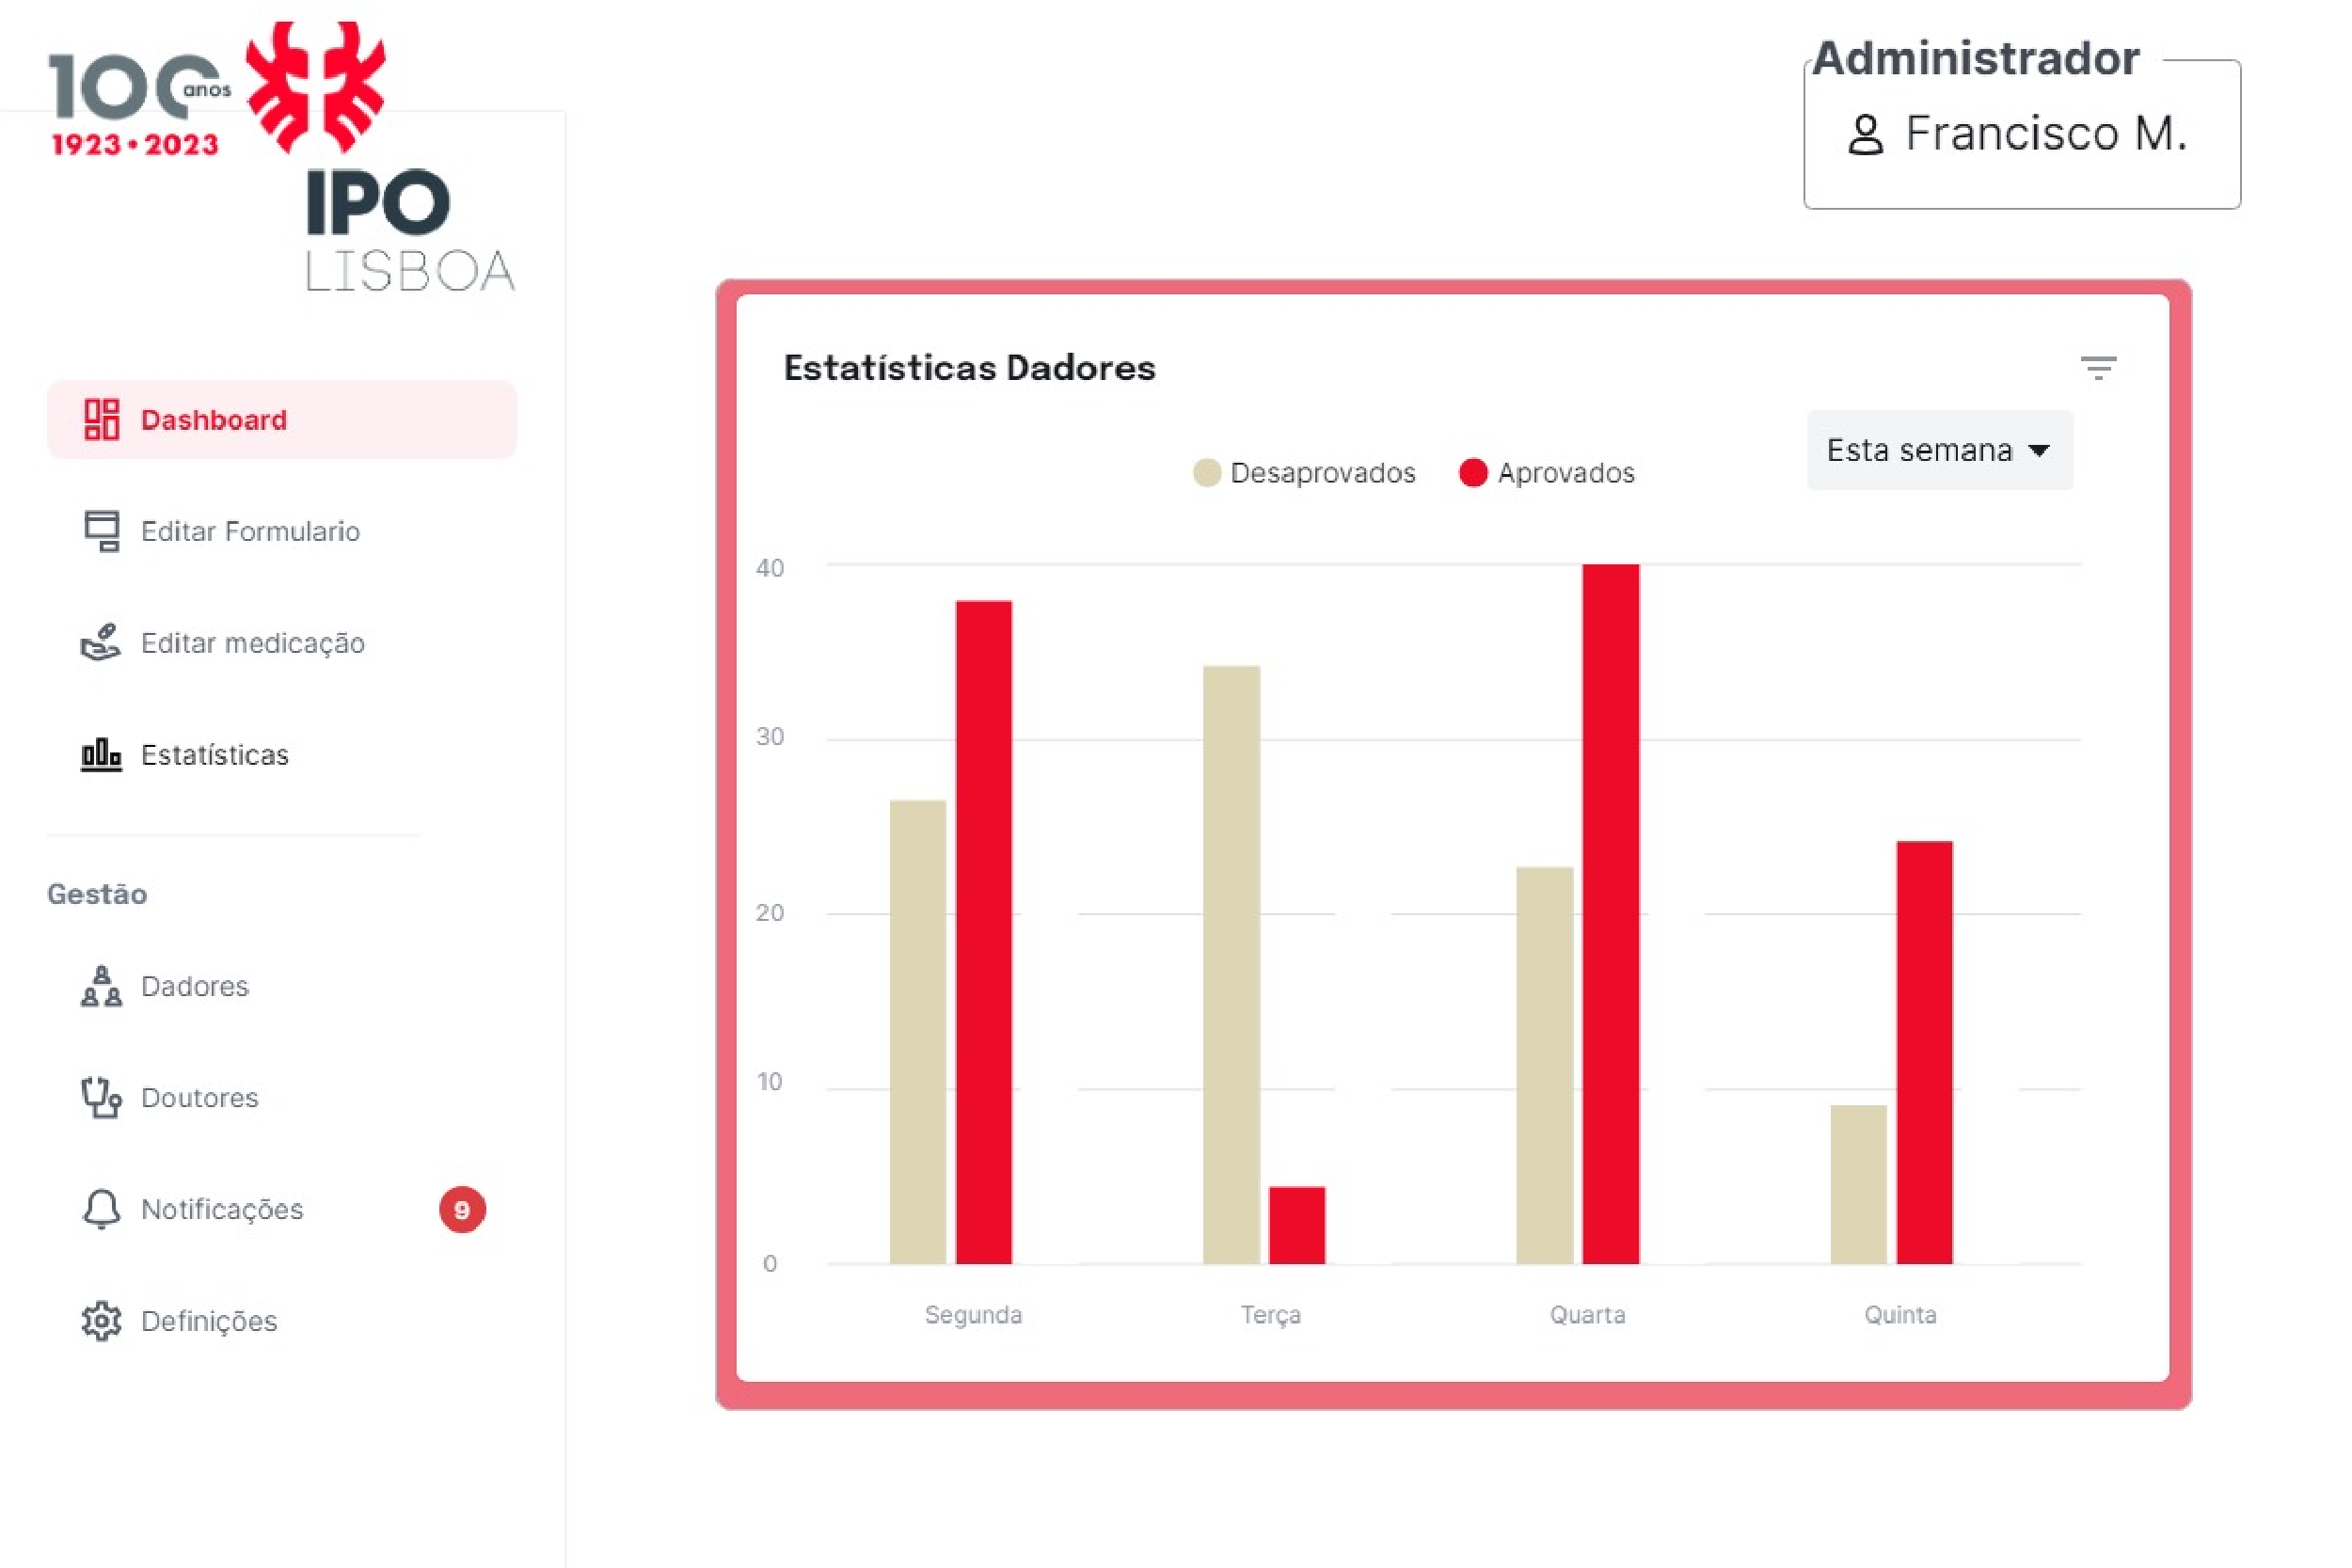
\includegraphics{./figures/Backoffice.pdf}}
	\end{center}
	\caption{Backoffice Page Mock.}\label{fig:backoffice}
\end{figure}




%\subsection{Form Services}
%
%The form service is responsible for managing the form resources.
%Figure ~\ref{fig:form_services} is a diagram that shows the architecture of the form services.
%
%\begin{figure}[htbp]
%	\begin{center}
%		\resizebox{150mm}{!}{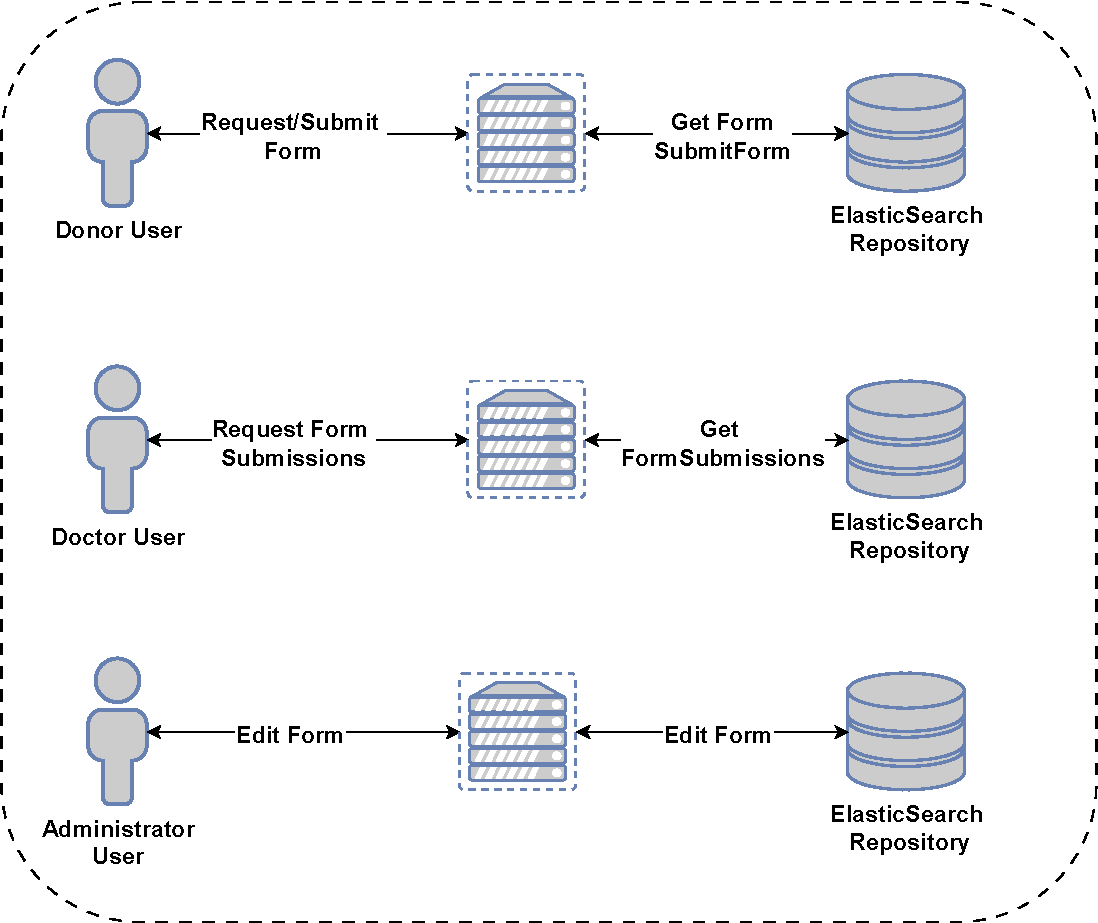
\includegraphics{./figures/formServices.pdf}}
%	\end{center}
%	\caption{Final Form Data Structure.}\label{fig:form_services}
%\end{figure}


% Capitulo 4
%%
% Capítulo 3
%
\chapter{Technologies} \label{cap:technologies}

 In this chapter, we introduce the key technologies that underpin the various components of the DADIVA IPO Platform. We will explain each technology's purpose and relevance within the context of our project. The discussion is organized into three main sections: backend technologies, frontend technologies, and version control tools. Our choices were significantly influenced by the experience and knowledge gained during our bachelor's degree in computer science:
\begin{itemize}
	\item Introduction to Web Programming (Introdução à Programação na Web) - Express.js;
	\item Web Application Development (Desenvolvimento de Aplicações Web)- Docker, React, Material-UI, Webpack, Spring;
	\item Systems Virtualization Techniques (Técnicas de Virtualização de Sistema) - Docker;
	\item Software Laboratory (Laboratório de Software) - Docker;
	\item Informatic Security (Segurança Informática) - RBAC;
	\item Git and Github were used during most of the course.
\end{itemize}

\section{Backend Technologies}

The backend technologies used in the DADIVA IPO platform share conceptual similarities with those we encountered in courses such as Web Application Development and Introduction to Web Programming. These technologies form the server-side components responsible for data processing, database management, and API integrations. In this section, we will provide a comprehensive overview of the key backend technologies employed in our project, highlighting their functionalities, benefits, and relevance to our system. We will also explore how these technologies collaborate to ensure the seamless operation and performance of the DADIVA IPO platform.

The programming language used for the backend is C\#. This general-purpose, object-oriented language was selected for several reasons:
\begin{itemize}
	\item Industry Relevance: C\# is part of the technology stack at Cofidis, aligning our project with industry standards;
	\item Learning Opportunity: Using C\# in this project provided us with valuable experience in a new language, preparing us for diverse development environments post-graduation;
	\item Robustness: C\# is well-suited for building scalable and maintainable backend systems, offering strong type safety and extensive libraries.
\end{itemize}

While C\# was our final choice, we considered other languages based on our coursework experience:
\begin{itemize}
	\item Kotlin: Extensively used during our course, Kotlin is known for its modern syntax and interoperability with Java;
	\item Java: A staple language for backend development, Java shares many characteristics with C\#, making it another viable option.
\end{itemize}

However, C\# presented a unique and interesting challenge, offering a fresh perspective compared to the more familiar alternatives.

\subsection{.NET}
.NET is a comprehensive development framework created by Microsoft. It serves as the backbone for building a variety of applications, including web, mobile, desktop, gaming, and Internet of Things (IoT) applications.

.NET provides a built-in dependency injection container that is straightforward to use. This container is integrated into various application types, including ASP.NET Core, and is conceptually similar to Spring, as well as a Role Based Access Control(RBAC). This framework also allows to create Minimal API's which are controller free API's similar to the Express.js API created during Introduction to Web Programming.

\subsection{Docker}

Docker is an open-source project which wraps and extends Linux containers technology to create a complete solution for the creation and distribution of containers.
The Docker platform provides a vast number of commands to conveniently manipulate
containers.

A container is an isolated, yet interactive, environment configured with all the dependencies necessary to execute an application. The use of containers brings advantages
such as:
\begin{itemize}
	\item Having little to no overhead compared to running an application natively, as it interacts directly with the host OS kernel and no layer exists between the application running and the OS;
	\item Providing high portability since the application runs in the environment provided by the container; bugs related to runtime environment configurations will almost certainly not occur;
	\item Running dozens of containers at the same time, thanks to their lightweight nature;
	\item Executing an application by downloading the container and running it, avoiding going through possible complex installations and setup.
\end{itemize}

To easily configure the virtual environment that the container hosts, Docker provides Docker images. Images are snapshots of all the necessary tools and files to execute an application. 
Containers can be started from images, the same way virtual machines run snapshots. To effortlessly distribute images, Docker provides registries. These are public or private stores where users may upload or download images. Docker provides a cloud-based registry service called DockerHub.

In addition to the Docker platform, we use Docker Compose to orchestrate the containers. Docker Compose is a tool for defining and running multi-container Docker applications. With Compose, we can define a multi-container application in a single file, then spin it up in a single command which does everything that needs to be done to get it running. Compose is especially useful in development environments, testing environments. 

We use Docker as an alternative for software containerization because it is the most well known, actively developed and supported in the area. Many frameworks already support it or are starting to support it.

\section{Frontend Technologies}\label{sec:frontend_tech}

\subsection{React}

React is a JavaScript library for building user interfaces. It is maintained by Facebook and a community of individual developers and companies. React can be used as a base in the development of single-page or mobile applications.

React is a component-based library, which means that the application is built by assembling components. Each component is a small piece of code that can be reused in different parts of the application. React is also declarative, which means that it is possible to describe the user interface without specifying how the user interface should be updated.

In DADIVA IPO, we use React to create the user interface. We also use React Router to manage the routing of the application. React Router is a collection of navigational components that compose declaratively with your application.

\subsection{JSON-Rules-Engine}

JSON-Rules-Engine is a library that enables the evaluation of business rules based on data inputs, providing a way to separate business logic from the core application code. Rules are defined in JSON format, making them easy to read, write, and maintain. The engine evaluates these rules against provided facts (data inputs) and triggers actions based on the results.

\subsection{Material-UI}

In addition to React, we also use Material-UI to create the user interface. Material-UI is a React component library that implements Google’s Material Design, which is a design language that combines the classic principles of successful design along with innovation and technology. Material-UI provides a set of components that can be used to create a user interface that follows the Material Design guidelines, such as buttons, cards, and tables. This makes it easier to create a consistent user interface.

\subsection{Webpack}

Webpack is a module bundler. It takes modules with dependencies and generates static assets representing those modules. Webpack is used to bundle JavaScript files for usage in a browser. It also provides a set of plugins that can be used to optimize the application, such as minification and code splitting.

In DADIVA IPO, we use Webpack to bundle the JavaScript files of the application, optimizing them for production. The technology also provides a development server, which is used to serve the application during development. We also use ts-loader to compile TypeScript files into JavaScript.

\section{DevOps Technologies}

\subsection{ Git and GitHub}
Git and GitHub are widely used version control tools that play a critical role in modern DevOps practices. Git is a distributed version control system that allows teams to efficiently manage changes to source code, track them over time and streamlines developer collaboration. GitHub, on the other hand, is a web-based hosting service for Git repositories that provides additional collaboration and project management features. Both of these technologies where extensively used trough our course.

\subsection{ Swagger }
Swagger ~\cite{Swagger} is an open-source framework that simplifies the design, documentation, and consumption of RESTful web services. It is widely used in the software development industry to create, visualize, and interact with API specifications. Swagger's comprehensive suite of tools and features enhances the development workflow, making it easier for developers to build and maintain APIs.

\subsection{ diagrams.net }
In the development of this report, the majority of the diagrams were created using diagrams.net ~\cite{diagrams.net}, also known as draw.io. Diagrams.net is a highly popular online diagramming tool that offers users the ability to design a wide variety of diagrams with ease and precision.
Some of diagrams.net's key features are:
\begin{itemize}
	\item \textbf{User-Friendly Interface}: Diagrams.net boasts an intuitive and user-friendly interface, making it accessible to both beginners and experienced users. The drag-and-drop functionality allows for quick creation and editing of diagrams.
	\item \textbf{Wide Range of Diagram Types}: The platform supports a diverse array of diagram types, including flowcharts, organizational charts, mind maps, network diagrams, UML diagrams, ER diagrams, and more. This versatility makes it a one-stop solution for most diagramming needs.
	\item \textbf{Customization Options}: Users can customize diagrams extensively with a variety of shapes, connectors, and styles. The tool offers a rich library of predefined shapes and templates that can be tailored to specific requirements.
	\item \textbf{Collaboration Capabilities}: Diagrams.net supports real-time collaboration, allowing multiple users to work on the same diagram simultaneously. This feature is particularly useful for team projects and collaborative work environments.
	\item \textbf{Integration and Compatibility}: The tool integrates seamlessly with popular cloud storage services like Google Drive, OneDrive, Dropbox, and GitHub. This ensures that diagrams can be easily saved, shared, and accessed from anywhere.
\end{itemize}

\subsection{ visily.ai }

Visily.ai~\cite{Visily} is a powerful design tool that leverages artificial intelligence to facilitate the creation of wireframes and prototypes for web and mobile applications. It is designed to help both designers and non-designers quickly produce high-quality visual representations of their ideas, and was used to produce the mockups show in section ~\ref{architecture_frontend}.
%
% Capítulo 4
%
\chapter{Data Model}\label{cap:data_model}
In this section we'll elaborate on the various entities that compose our application and their interactions.
The complete entity relationship diagram is present in Appendix \ref{er}.

\subsection{User}

As outlined in section \ref{sec:use_cases}, our application divides users in roles, with each role being able to perform specific actions, as such, the \textbf{User} entity is a supertype, with roles being the overlapping subtypes of user, as a user can occupy multiple roles, as illustrated in Figure \ref{fig:user_entity}.

\begin{figure}[h]
	\begin{center}
		\resizebox{160mm}{!}{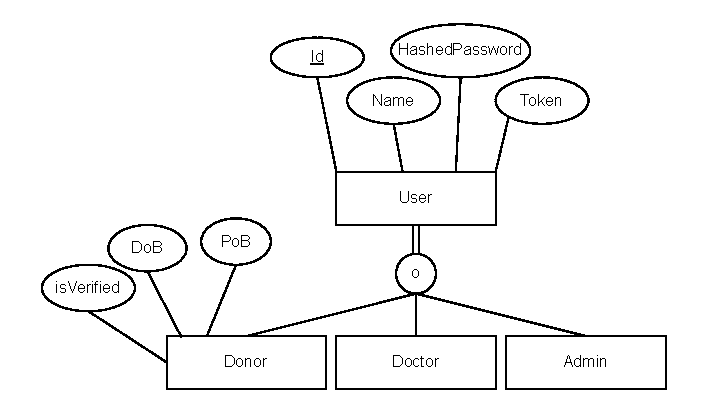
\includegraphics{./figures/User_Entity.pdf}}
	\end{center}
	\caption{User Entity.}\label{fig:user_entity}
\end{figure}

The \textbf{User} supertype contains the attributes that are common to all roles, which are as follows:

\begin{itemize}
	\item Id:A unique identifier which can be a passport or civil identification number;
	\item Name: the user's full name;
	\item HashedPassword: The user's password, stored securely as a hash, more details in section \ref{sec:security};
	\item Token: An authentication token for the user.
\end{itemize}

The \textbf{Donor} subtype contains some specific attributes, which are pertinent to this type, such as:
\begin{itemize}
	\item isVerified: boolean, indicates if donor supplied proof of identity;
	\item DoB: the donor's date of birth;
	\item PoB: the donor's place of birth;
\end{itemize}

\subsubsection{User relationships}

\begin{figure}[H]
	\begin{center}
		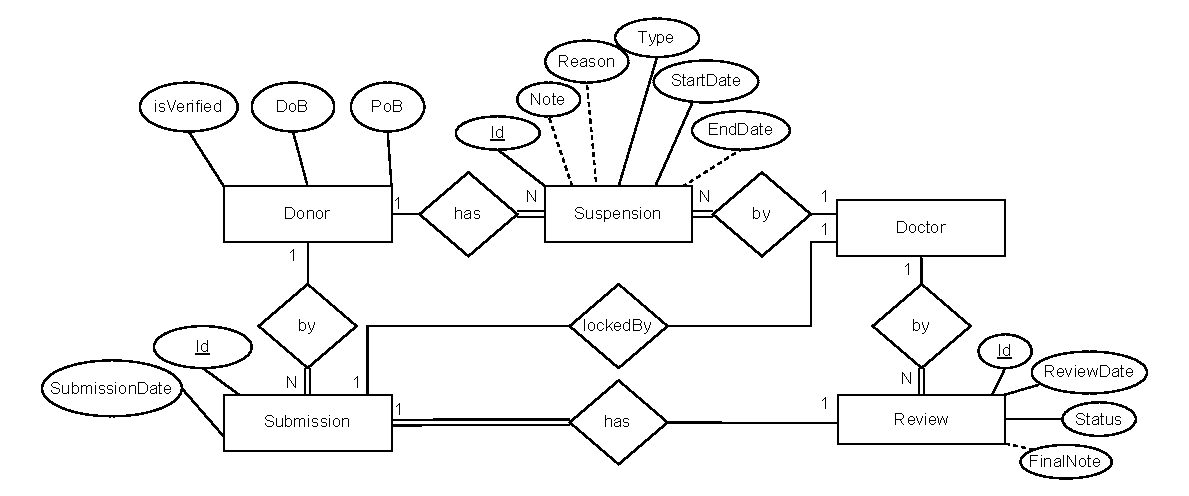
\includegraphics[width=\textwidth,height=\textheight,keepaspectratio]{./figures/User_Interactions.pdf}
	\end{center}
	\caption{User interactions.}\label{fig:user_interactions}
\end{figure}

%As mentioned before, a donor must be verified, this verification is done by an administrator upon first donation when a donor supplies proof of identity.
A \textbf{Donor} can be suspended, ie after a blood donation there's a 2 month waiting period until the next donation, this \textbf{Suspension} is created by a \textbf{Doctor}.
Each \textbf{Donor} can have multiple \textbf{suspensions}, ie multiples waiting periods after donations, and each \textbf{Doctor} can issue multiple \textbf{suspensions}.

The attributes used to characterize a \textbf{Suspension} are as follows:

\begin{itemize}
	\item \textbf{Id}:A unique identifier for the suspension;
	\item \textbf{Type}: Indicates whether the suspension is temporary or permanent;
	\item \textbf{StartDate}: The date when the suspension begins;
	\item \textbf{EndDate}: The date when the suspension ends, optional as permanent suspensions don't have an end date;
	\item \textbf{Reason}: An optional field to specify the reason for the suspension;
	\item \textbf{Note}: An optional note related to the suspension.
\end{itemize}

A \textbf{Donor} performs various pre-donation form \textbf{submissions}, which need to be reviewed by a \textbf{Doctor}, whom can \textbf{review} multiple \textbf{submissions},  with each \textbf{Submission} having a single \textbf{Review}.
The \textbf{Submission} entity's relationships are elaborated on in section \ref{sec:submission}.

A \textbf{Submission} is characterized by the date in which it was performed, \textbf{SubmissionDate}, and a unique identifier.

A review is characterize by the following attribute:
\begin{itemize}
	\item \textbf{Id}:A unique identifier for the Review;
	\item \textbf{ReviewDate}: The date in which the review was performed;
	\item \textbf{Status}: ;
	\item \textbf{FinalNote}: Optional, potential notes;
\end{itemize}





\subsection{Admin}

\begin{figure}[h]
	\begin{center}
		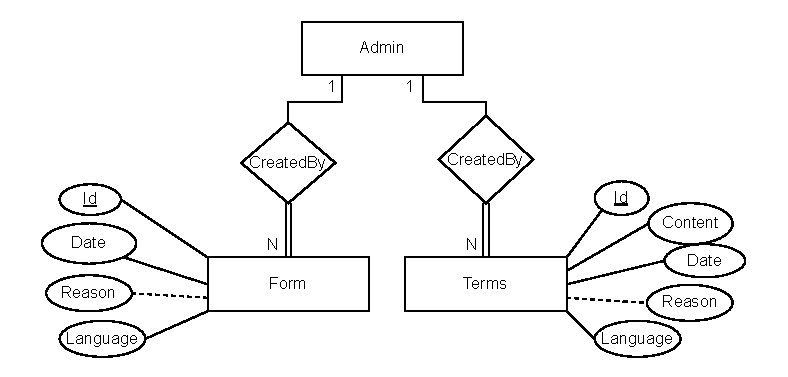
\includegraphics[width=\textwidth,height=\textheight,keepaspectratio]{./figures/Admin_Entity.pdf}
	\end{center}
	\caption{User interactions.}\label{fig:admin_entity}
\end{figure}

An \textbf{Admin} can create multiple pre-donation \textbf{forms} and multiple legal \textbf{terms} for the donation.
The \textbf{Form} entity has more relationships, but to preserve this section's scope that information is omitted but is available in section \ref{sec:form}.

The \textbf{Form} entity is characterized by the following attributes:
\begin{itemize}
	\item \textbf{Id}:A unique identifier for the form;
	\item \textbf{CreatedAt}: The date in which the form was created;
	\item \textbf{Title}: The title of the form, for ease of identification;
	\item \textbf{Language}: The language of the form stored in ISO 639-3;
	\item \textbf{isActive}: Indicates if this form is the one being presented to the donors, only one form can be active at any time for a given language;
\end{itemize}

The \textbf{Terms} entity is characterized by the following attributes:
\begin{itemize}
	\item \textbf{Id}:A unique identifier for the terms;
	\item \textbf{Content}: The actual terms;
	\item \textbf{CreatedAt}: The date in which the terms were created;
	\item \textbf{Title}: The title of the terms, for ease of identification;
	\item \textbf{Language}: The language of the terms;
	\item \textbf{isActive}: Indicates if these terms are being presented to the donors, only one of these entities can be active at any time;
\end{itemize}





\subsection{Form relationships}\label{sec:form}

\begin{figure}[h]
	\begin{center}
		\resizebox{160mm}{!}{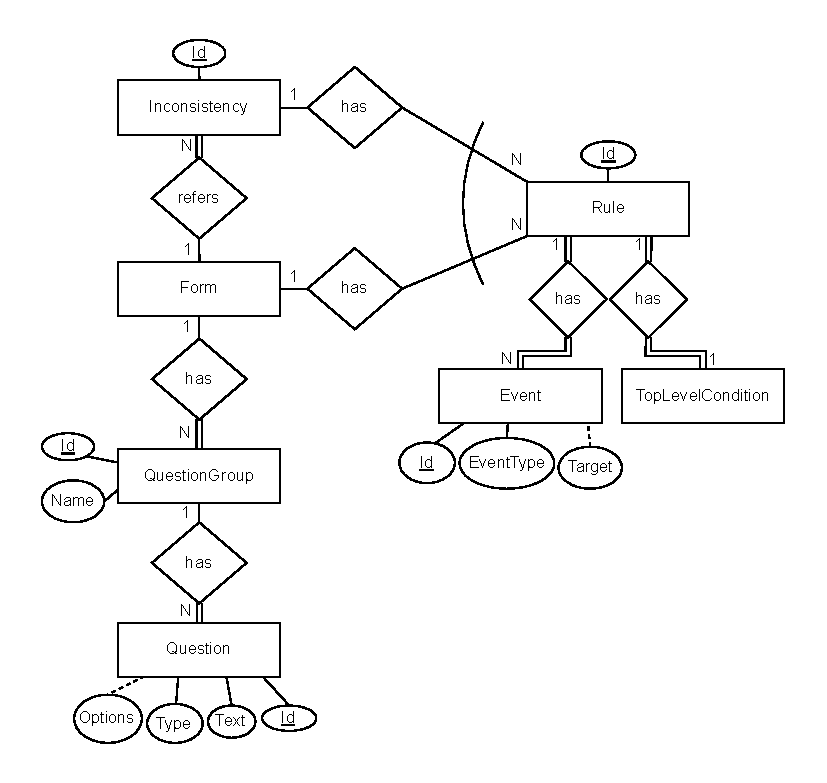
\includegraphics{./figures/Form_Entity.pdf}}
	\end{center}
	\caption{Form Entity.}\label{fig:form_entity}
\end{figure}

A \textbf{Form} is composed of a group of \textbf{questions}, this group represents a theme, and a set of \textbf{rules}, as such it has a one to many relationship with these entities.
For the sake of simplicity a rule can be defined as a logical condition, the \textbf{TopLevelCondition} entity in Figure \ref{fig:form_entity}, that triggers an event when met,ie when a donor answers that he has traveled abroad a subsequent question appears asking to which country, a further explanation of the entities that make up these conditions is presented in section \ref{sec:conditions}.

A \textbf{QuestionGroup} entity has the following attributes:
\begin{itemize}
	\item \textbf{Id}: The group's unique identifier;
	\item \textbf{Name}: The theme of the group, ie travel, health, previous donations, etc;
\end{itemize}

Logically, a \textbf{QuestionGroup} as a one to many relationship with the \textbf{Question} entity.
A \textbf{Question} entity is characterized by the following attributes:
\begin{itemize}
	\item \textbf{Id}: The question's unique identifier;
	\item \textbf{Text}: The actual question;
	\item \textbf{Type}: The type of accepted answer, ie boolean, text, multiple values, etc;
\end{itemize}

An \textbf{Event} entity is characterized by the following attributes:
\begin{itemize}
	\item \textbf{Id}: The event's unique identifier;
	\item \textbf{EventType}: The action the event performs, ie hide/show a question, allow navigation to next group, etc ;
	\item \textbf{Target}: Optional, the target of the action, ie the question to be hidden or displayed;
\end{itemize}

The \textbf{Inconsistency} entity represents a logical fallacy in sets of answers, eg a donor stating the they never traveled outside of Portugal but also stating that they've resided outside of Portugal.
This entity is compromised of a single identifying attribute,Id, and has a one to many relationship with the \textbf{Rule} entity. 


%\subsection{Inconsistency}
%
%\begin{figure}[H]
%	\begin{center}
	%		\resizebox{160mm}{!}{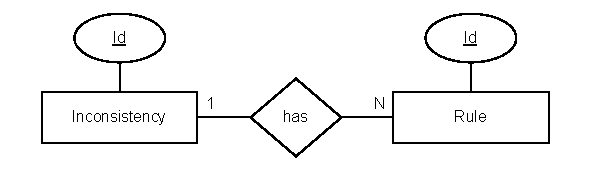
\includegraphics{./figures/Inconsistency_Entity.pdf}}
	%	\end{center}
%	\caption{Form Entity.}\label{fig:inconsistency_entity}
%\end{figure}
%
%The inconsistency entity, illustrated in Figure \ref{fig:inconsistency_entity} represents sets of answers that are illogical, ie a donor stating that they've never traveled outside of Portugal but also stating that they've resided outside of Portugal.
%This entity is compromised of a single identifying attribute,Id, and has a one to many relationship with the rule entity,mentioned in subsection \ref{sec:form}.








%\subsection{Rule}\label{sec:rule_entity}
%
%\begin{figure}[H]
%	\begin{center}
	%		\resizebox{160mm}{!}{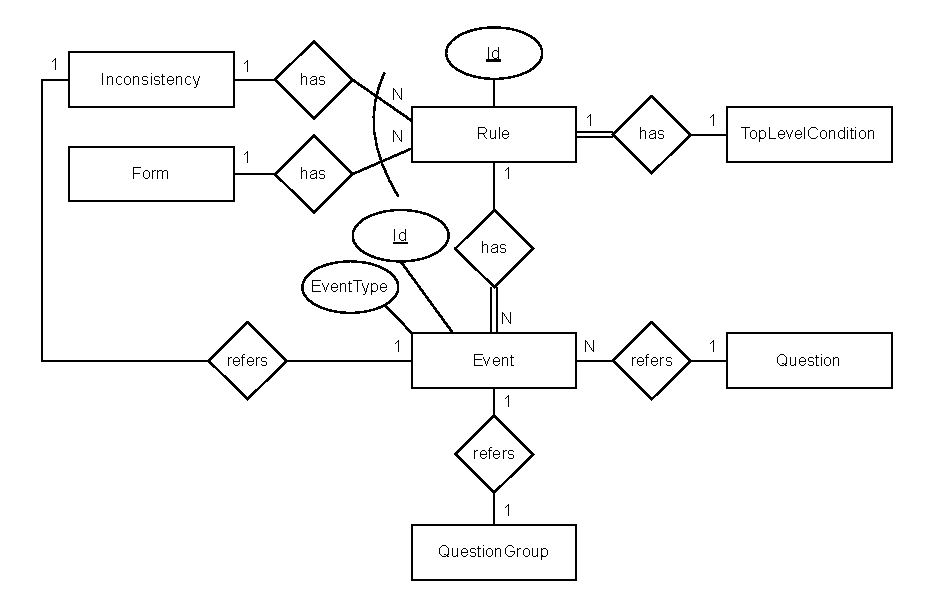
\includegraphics{./figures/Rule_Entity.pdf}}
	%	\end{center}
%	\caption{Form Entity.}\label{fig:rule_entity}
%\end{figure}
%
%The rule entity, illustrated in Figure \ref{fig:rule_entity}, has a single identifying attribute, Id, and  can be a part of a form or an inconsistency, as mentioned before.
%It has a one to one relationship with the top level condition entity, which is further elaborated in subsection \ref{conditions}, but, for now, can simply be described as the logical premises of the rule.
%
%If the logical premises are met one or more events might be triggered, hence the event entity and the rule entity have a one to many relationship.
%
%The event entity has the following attributes:
%\begin{itemize}
%	\item Id: The event's unique identifier;
%	\item EventType: The consequence of this event, ie show a question, enable the next question group, or point out inconsistent responses;
%\end{itemize}
%
%As described by the EventType attribute, and event entity can reference a question, a question group or an inconsistency.

\subsection{Conditions}\label{sec:conditions}

\begin{figure}[h]
	\begin{center}
		\resizebox{160mm}{!}{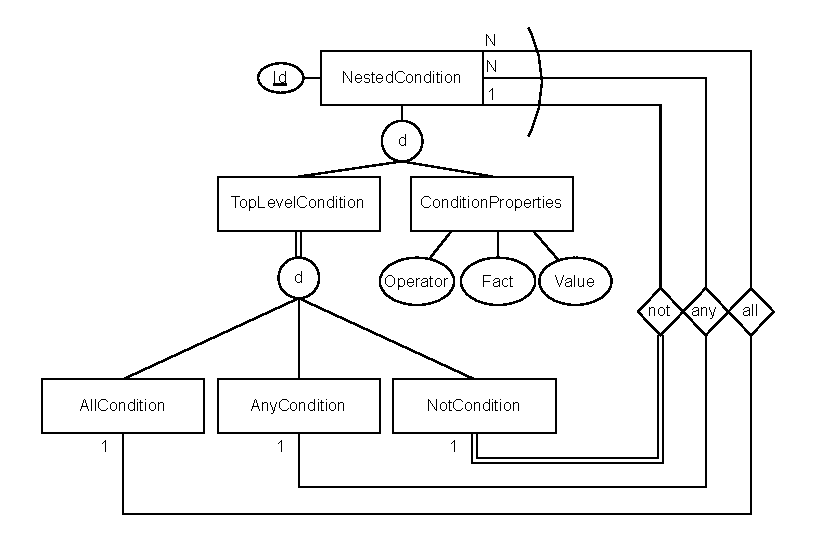
\includegraphics{./figures/Condition_Entity.pdf}}
	\end{center}
	\caption{Condition Entity.}\label{fig:condition_entity}
\end{figure}

The entities and relationships mentioned in this section reflect the types belonging to the \textbf{JSON-Rules-Engine}.
The  \textbf{NestedCondition} entity is a supertype of the \textbf{TopLevelCondition} entity and the \textbf{ConditionProperties} entity.
As the \textbf{TopLevelCondition} entity is a supertype of the \textbf{AllCondition}, \textbf{AnyCondition} a \textbf{NotCondition} entities, it can be seen as a representation of logical operators. As illustrated in Figure \ref{fig:condition_entity}, the \textbf{AllCondition} and \textbf{AnyCondition} entities have a one to many relationship with the \textbf{NestedCondition}, while the \textbf{NotCondition} as a one to one relationship, this means the \textbf{all} and \textbf{any} conditions can have multiple conditions nested inside them while the \textbf{not} condition can have a single condition nested inside it, which allows for the creation of complex boolean expressions.

The \textbf{ConditionProperties} entity represents a logical evaluation and has the following attributes:
\begin{itemize}
	\item \textbf{Operator}: The logical operator of the evaluation, ie equal, less than, greater than, etc;
	\item \textbf{Fact}: The id of the question being evaluated;
	\item \textbf{Value}: The expected value of the question being referenced.
\end{itemize}





\subsection{Submission}\label{sec:submission}

\begin{figure}[h]
	\begin{center}
		\resizebox{160mm}{!}{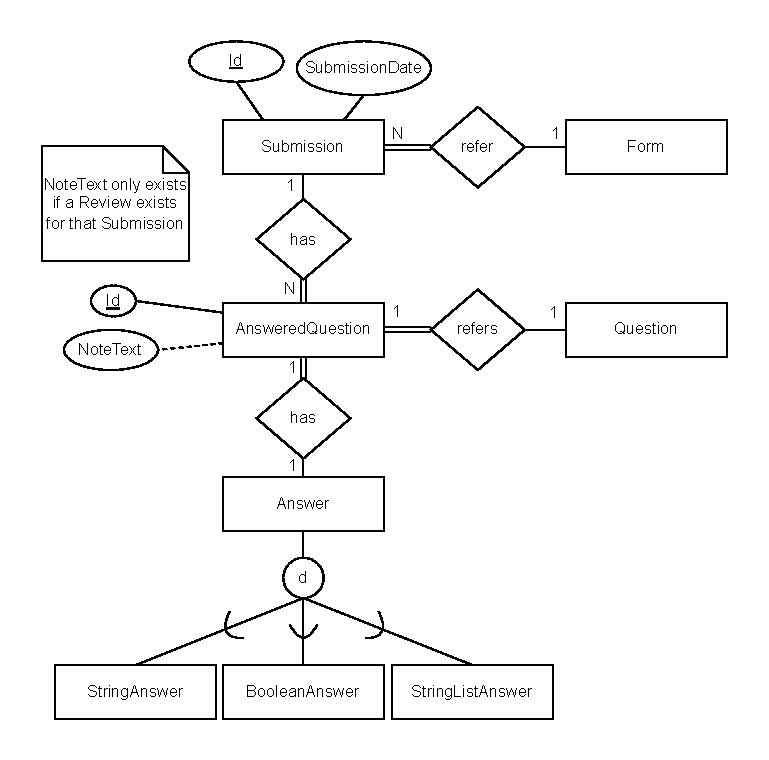
\includegraphics{./figures/Submission_Entity.pdf}}
	\end{center}
	\caption{Submission Entity.}\label{fig:submission_entity}
\end{figure}

As illustrated in Figure \ref{fig:submission_entity}, the \textbf{Submission} entity as a relationship with the \textbf{Form} entity, since a given submission pertains to a certain version of the form which changes overtime, and with the \textbf{AnsweredQuestion} entity,this entity has a \textbf{NoteText} attribute, which is optional, and represents a doctor note about the answer provided and a relationship with the \textbf{Question} entity, since every answer must refer to a question in the form.
The \textbf{AnsweredQuestion} entity also has a relationship with the \textbf{Answer} entity which is a supertype representing the possible values for the form's answers.



%\subsection{Change Log}
%
%\begin{figure}[H]
%	\begin{center}
	%		\resizebox{160mm}{!}{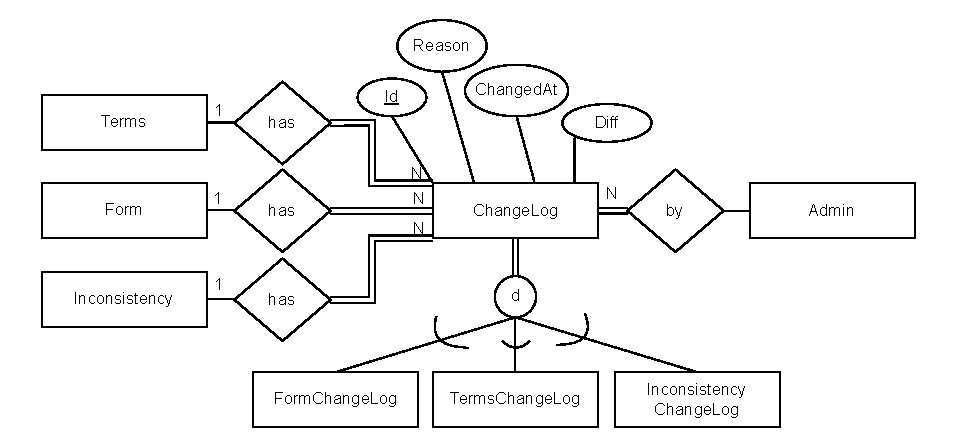
\includegraphics{./figures/ChangeLog_Entity.pdf}}
	%	\end{center}
%	\caption{ChangeLog Entity.}\label{fig:changelog_entity}
%\end{figure}
%
%To enforce admin accountability for \textbf{term}, \textbf{form} and \textbf{inconsistency} changes the \textbf{ChangeLog} entity was created and is illustrated in Figure \ref{fig:changelog_entity}.
%
%This entity has relationships with all the entities that are subjected to change and with the \textbf{Admin} entity that performed the changes.
%
%The \textbf{ChangeLog} entity serves as a supertype of the possible changes to the system, and it as the following attributes:
%\begin{itemize}
%	\item \textbf{Id}: The ChangeLog's unique identifier;
%	\item \textbf{Reason}: Optional, reason for the change;
%	\item \textbf{ChangedAt}: The date the change was performed;
%	\item \textbf{Diff}: What was changed;
%\end{itemize}

\subsection{Manual Information}

\begin{figure}[h]
	\begin{center}
		\resizebox{160mm}{!}{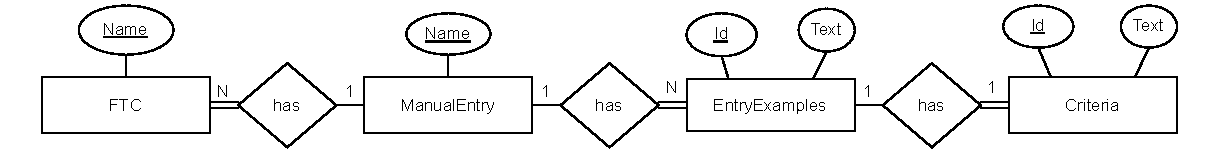
\includegraphics{./figures/Manual_Entity.pdf}}
	\end{center}
	\caption{Manual Entity.}\label{fig:manual_entity}
\end{figure}

To allow doctors to search for medication interactions with blood donations and to perform the risk vector analysis we created the \textbf{FTC} entity which is the pharmaco-therapeutic classification of the medication.
This entity has an identifying \textbf{Name} attribute, which is the name for this group of medications, e.g. analgesics and antipyretics, non steroidal anti inflammatories, etc.

The \textbf{ManualEntry} entity has an identifying \textbf{Name} attribute, which is the name used to group medications in the manual.

The \textbf{FTC} and \textbf{ManualEntry} entities have a many to one relationship as the names used in the manual might refer to more than one classification, and will possibly not have a match with any \textbf{FTC}.

The \textbf{EntryExamples} entity represents the examples presented in the manual for each entry, ie in the 2022 manual the analgesics entry contains two examples "Paracetamol, Ben U Ron, Tramadol..." and "Opioid Analgesics", so this entity has a many to one relationship with the \textbf{ManualEntry} entity and an attribute \textbf{Text}, with the examples.

Finally the \textbf{Criteria} entity which refers to whether a donor is able to donate blood or should be suspended, and whether that suspension is temporary or permanent if he's taken this medication. This entity as a one to one relationship with \textbf{EntryExamples} entity, as the evaluation of blood donation capabilities is dependent on these examples, since different medications within the same classification can lead to distinct outcomes.

\subsection{Locks}\label{sec:lock_entity}

\begin{figure}[H]
	\begin{center}
		\resizebox{160mm}{!}{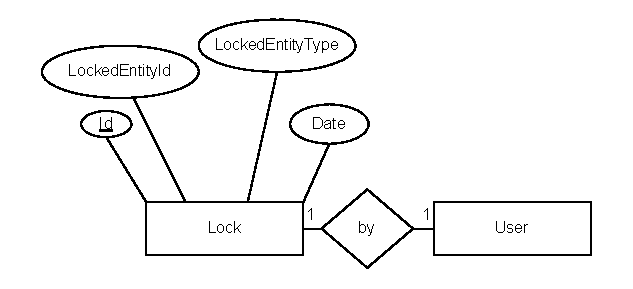
\includegraphics{./figures/Lock_Entity.pdf}}
	\end{center}
	\caption{Lock Entity.}
\end{figure}

To avoid concurrent manipulation of resources we created the \textbf{Lock} entity. This entity has a
one to one relationship with the \textbf{User} holding the lock for this resource and has the following
attributes:

\begin{itemize}
	\item \textbf{Id}: The unique identifier for this lock
	\item \textbf{LockedEntityId}: The identifier for the resource being locked;
	\item \textbf{LockedEntityType}: The type of resource being locked, i.e. submission, form, terms;
	\item \textbf{Date}: The date when the resource was locked .
\end{itemize}

% Capitulo 5
%
% Capítulo 5
%
\chapter{Frontend Implementation} \label{cap:frontend_implementation}

This chapter focuses on the frontend implementation, which is responsible for data visualization and user interaction. The main objective is to provide an intuitive interface that allows various users to fulfill the use cases outlined in Section ~\ref{sec:use_cases}. The frontend is built using TypeScript \cite{TypeScript} and React\cite{React}, incorporating the JSON-Rules-Engine to enforce the form's rules and makes use of Material UI \cite{Material_UI} components to build the UI. In the sections that follow, we will dive into the detailed interactions between the components and how the state management is handled throughout the application.

Figure \ref{fig:frontend_implementation} shows a simplified view of the component structure used in the frontend of the application. At the top, we have the I18nextProvider, which handles the user's language preferences, ensuring internationalization support. Below that, the AuthnContainer manages session information, such as user authentication and credentials.

The App component is the main container of the application, housing the FormPage and useNewForm, which are responsible for displaying the form to the donor users and managing its state using the JSON-Rules-Engine. 

The EditFormPage and useEditFormPage components handle the back-office form display and allow administrators to modify the form structure.

Additionally, the Editor component is used in the EditTermsPage, providing a user-friendly interface for administrators to modify terms and conditions. This interface is integrated with a rich-text editor to allow flexibility in content editing.

The sections below will go into more detail about each of these components:

\begin{itemize}
	\item I18nextProvider: Manages language preferences for the application (Section \ref{I18n_component}).
	\item AuthnContainer: Handles session information (Section \ref{authcontainer}).
	\item FormPage \& useNewForm: Manages donor forms and their state using the JSON-Rules-Engine (Section \ref{form_implementation}).
	\item EditFormPage \& useEditFormPage: Manages the display and editing of forms for administrators in the back-office (Section \ref{edit_form}).
	\item Editor: Used in the EditTermsPage for editing terms and conditions (Section \ref{edit_terms}).
\end{itemize}

\begin{figure}[h]
	\begin{center}
		\resizebox{60mm}{!}{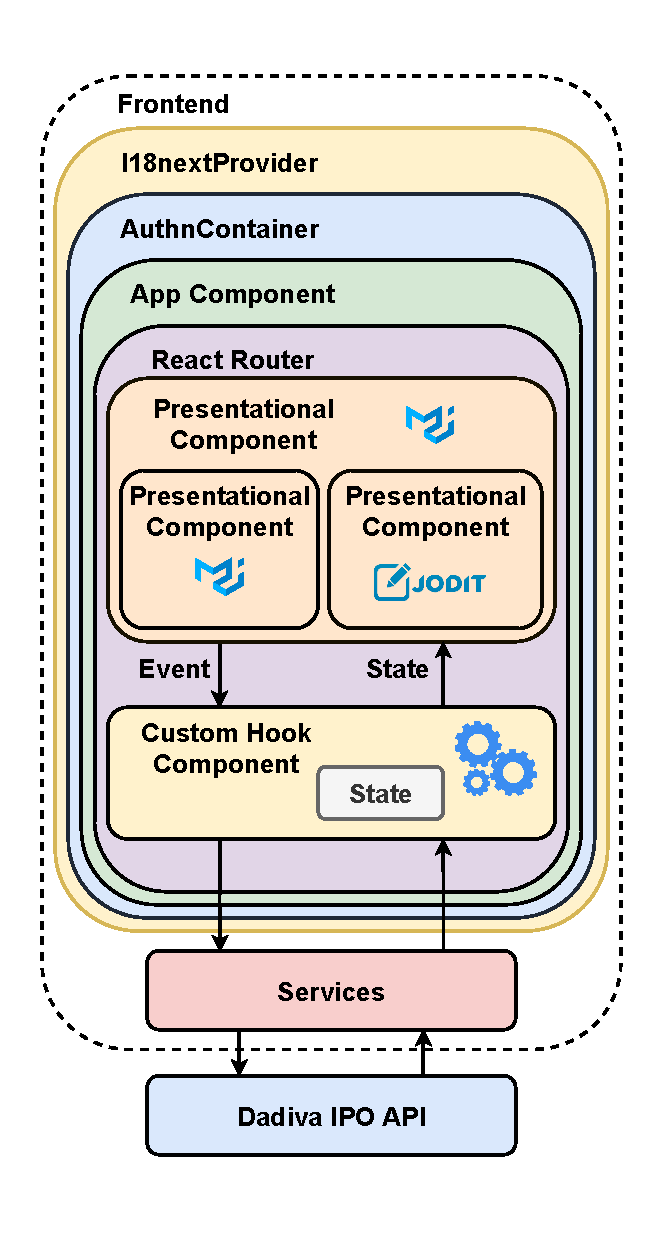
\includegraphics{./figures/frontend_implementation.pdf}}
	\end{center}
	\caption{Simplified Component interaction and organization.}\label{fig:frontend_implementation}
\end{figure}

\newpage

\section{Structure}

The frontend structure is as follows:

\begin{itemize}
	\item src: contains the source code of the application;
	\item public: contains the static files of the application;
	\item package.json:  contains the dependencies of the application;
	\item tsconfig.json: contains the TypeScript configuration;
	\item webpack.config.js:  contains the Webpack configuration.
\end{itemize}

The src folder is then subdivided into multiple folders/files, each being responsible for a different functionality of the application:

\begin{itemize}
	\item components: contains the components of the pages;
	\item domain: contains the domain objects;
	\item pages:  contains the application's pages, each containing various components;
	\item services: contains the services that communicate with the backend application;
	\item session: contains the code needed to maintain a user session.
	\item utils:  contains general utility functions.
\end{itemize}

It should be noted that, folders within the components folder may contain further utils, containing utility functions that are specially pertinent for that component and shouldn't necessarily be in the general utils. 

Furthermore, besides the aforementioned folders, the src folder also contains an index.tsx and App.tsx files. The index.tsx file is the entry point for the application meanwhile the App.tsx is the main component of the React application.


\section{Services}

The frontend services are responsible for communicating with the backend application and, as such, each frontend service has a backend counterpart.

To facilitate this communication we used the Fetch API \cite{Fetch_API}, which enables asynchronous resource requests by returning a promise that resolves to a response for that request.

To expedite, and reduce the code for, the api resource requests we created a fetchAPI function that accepts the request parameters and return a promise that will resolve to the requests response, this function can also handle errors if the response's status code isn't in the 200 family.

To further abstract the api calls,  the fetchAPI function was encapsulated within functions that represent specific HTTP methods, such as GET, POST, PUT and DELETE.

\newpage

\section{Components}

A simplified view of the component tree is presented in Figure ~\ref{fig:reactComponentTree}.
In this chapter we'll mainly focus on the:
\begin{itemize}
	\item \textbf{I18nextProvider}: manages the language preferences of the user;
	\item \textbf{AuthnContainer}: manages the session information;
	\item \textbf{FormPage \& useNewForm}: used to display form to the donor and manage it's state using JSON-Rules-Engine;
	\item \textbf{EditFormPage \& useEditFormPage}:  displays form in the backoffice, to the administrators, and allows to perform change's to the structure, also manage it's state;
	\item \textbf{Editor}: used to display the terms to the administrators and allows to change them. 
\end{itemize}

\begin{figure}[h]
	\begin{center}
		\resizebox{130mm}{!}{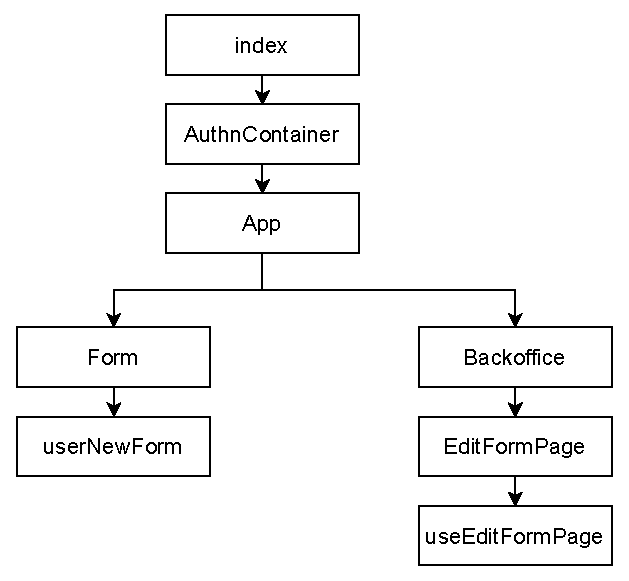
\includegraphics{./figures/reactComponentTree.pdf}}
	\end{center}
	\caption{Simplified React Component Tree.}\label{fig:reactComponentTree}
\end{figure}

When suitable there will be figures to illustrate the visuals of these components, a more complete list of the visuals for all components is available in Appendix \ref{UI}.
\subsection{I18nextProvider}\label{I18n_component}

The I18nextProvider component is part of the i18next library ecosystem, which is used for internationalization (i18n) in JavaScript applications. The purpose of the I18nextProvider component is to integrate i18next into React applications by providing the i18n instance to the component tree.

By accessing the i18n instance, we can set the desired language for the application. This is useful for both the frontend and to request certain resources from the backend, i.e. requesting the resource with the user's language preferences, or default to a certain resource if that isn't available.


\subsection{AuthnContainer}\label{authcontainer}
The AuthnContainer component plays a crucial role in enabling user authentication and consequent storage of the authentication information within the application state.

To do so it uses the React Context API \cite{React_Context_API}, which allows to pass data trough the component tree without having to pass props down manually at every level, thus enabling seamless data sharing between components.

The Session type describe a user's session, i.e. their name and nic. The SessionManager type acts as a wrapper, containing both the session and the methods to manage it, i.e. set a session and delete it.

The AuthContainer component wraps it's child components within it's LoggedInContext.Provider, providing the session manager instance and it's methods as the context value, making the authentication information available throughout the component tree.

\newpage
\subsection{FormPage \& useNewForm}\label{form_implementation}

The concepts in this section build upon those discussed in Section \ref{arc_jre}. It is advised to refer to that section for a thorough understanding.

The FormPage is responsible for form display to donor users. It leverages the useNewForm hook.

The useNewForm hook is a custom React hook designed to manage the state and logic of the form within the frontend application. This hook integrates several important functionalities, including handling form data, managing user interactions, and executing business rules, making it a critical part of the form-handling process.

To do this the hook makes use of the JSON-Rules-Engine \cite{JSON-Rules-Engine} and states, mainly: 
\begin{itemize}
	\item \textbf{showQuestions:} stores the questions that are being displayed;
	\item \textbf{canGoNext:} stores if the next group of questions should be available,  by default false when initializing;
	\item \textbf{canGoReview:} stores if all questions where answered and the form can be reviewed, by default false when initializing;
	\item \textbf{formAnswers:} stores all the answers given at any point.
\end{itemize}

Figure \ref{fig:form_implementation} illustrates this process which has the following steps:

\begin{itemize}
	\item \textbf{Fetch Form (Step 1):} The form data is fetched from the Services layer and passed to the useNewForm hook.
	\item \textbf{Set Facts and Rules (Step 2):} Inside the useNewForm hook, the form’s data is divided into facts (user's answers) and rules (logic for navigation and question visibility). These are added to a rule engine which runs via the function engine.run().
	\item \textbf{Handle Events (Step 3):} The rule engine emits events that determine question visibility and navigation options.
	\item \textbf{Update State (Step 4):} The FormPage component displays the form questions and buttons (e.g., "Next Group", "Review") based on the current state, showing the appropriate group of questions.
	\item \textbf{Update Form Answers (Step 5):} As users interact, their answers update the formAnswers state, which triggers the rule engine to re-evaluate, ensuring the form behaves as expected.
\end{itemize}

\begin{figure}[h]
	\begin{center}
		\resizebox{150mm}{!}{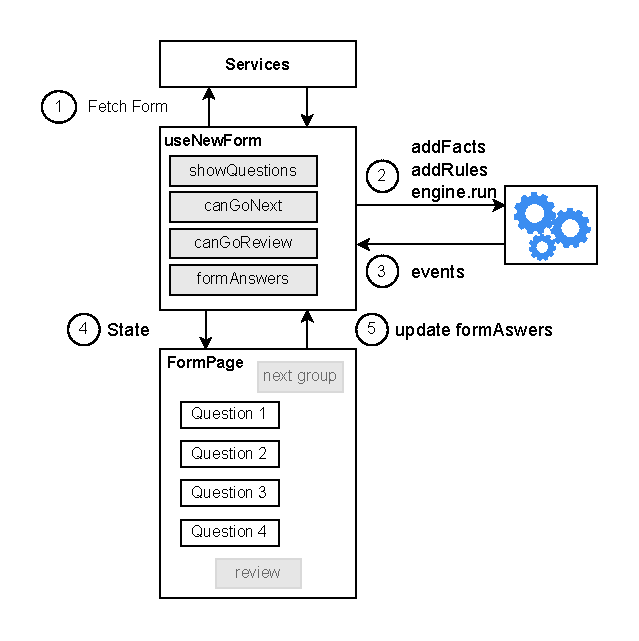
\includegraphics{./figures/JRE_implementation.pdf}}
	\end{center}
	\caption{Form implementation.}\label{fig:form_implementation}
\end{figure}

To make sure all questions that should show by default are visible the form has a rule, per question, in which the top level condition, no matter the type, is empty with an event of type showQuestion and referring to the question that should be visible by default, as illustrated in Listing \ref{default_question}.
Once the engine is run, these conditions are met and the respective events are returned.

\begin{lstlisting}[style=sharpc, caption={Condition for visible by default questions}, label={default_question}]
conditions: {
	any: [],
},
event: {
	type: 'showQuestion',
	params: {
		id: 'visibleByDefault'
	},
}
\end{lstlisting}

A view of this component is illustrated in Figures \ref{fig:form1} through \ref{fig:form3}.

\begin{figure}[h]
	\begin{center}
		\resizebox{120mm}{!}{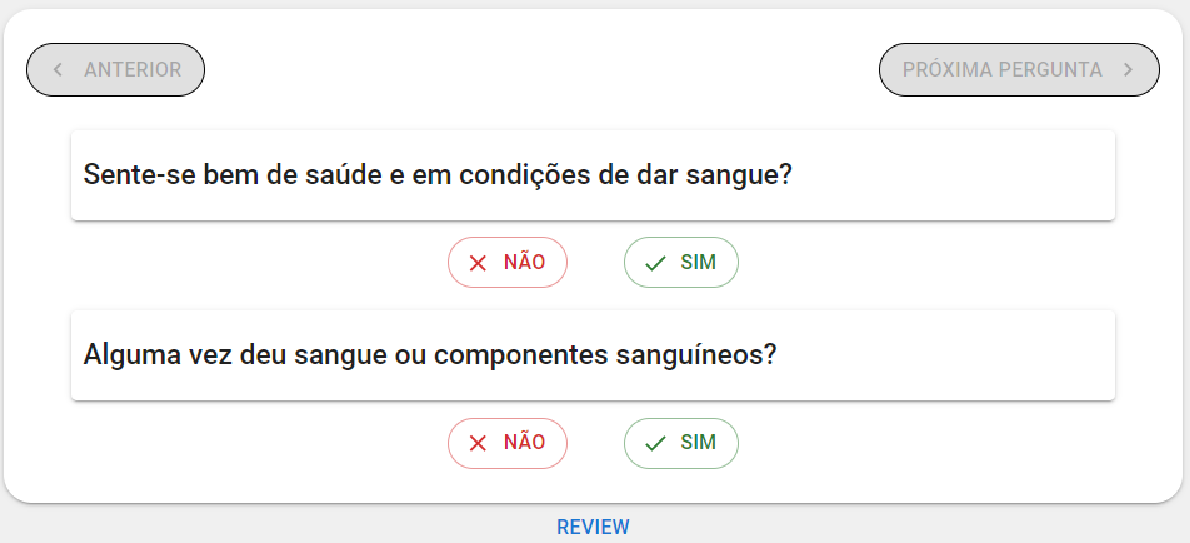
\includegraphics{./figures/Form1.pdf}}
	\end{center}
	\caption{Form Page with no answer.}\label{fig:form1}
\end{figure}

\begin{figure}[h]
	\begin{center}
		\resizebox{120mm}{!}{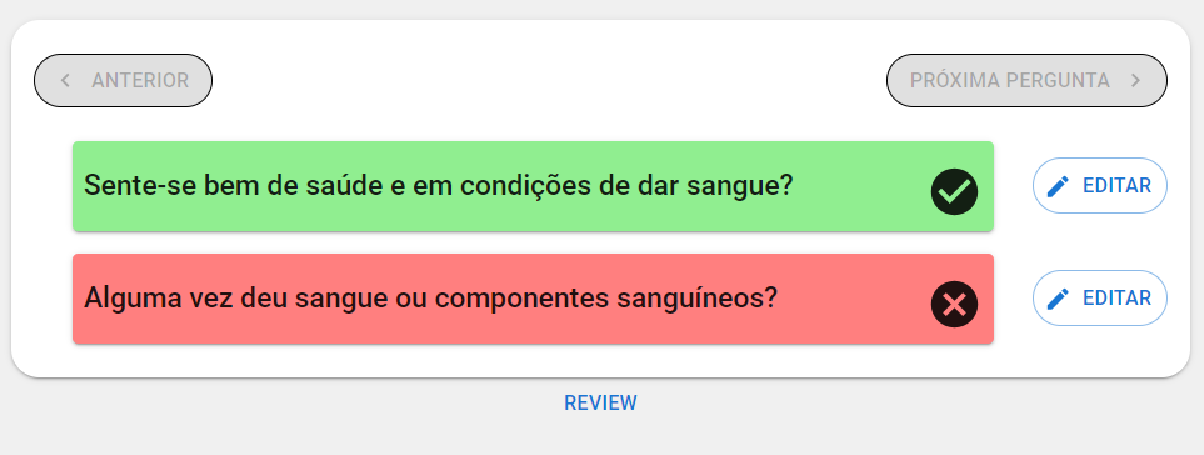
\includegraphics{./figures/Form2.pdf}}
	\end{center}
	\caption{Form Page with answers and no sub questions.}\label{fig:form2}
\end{figure}

\begin{figure}[H]
	\begin{center}
		\resizebox{120mm}{!}{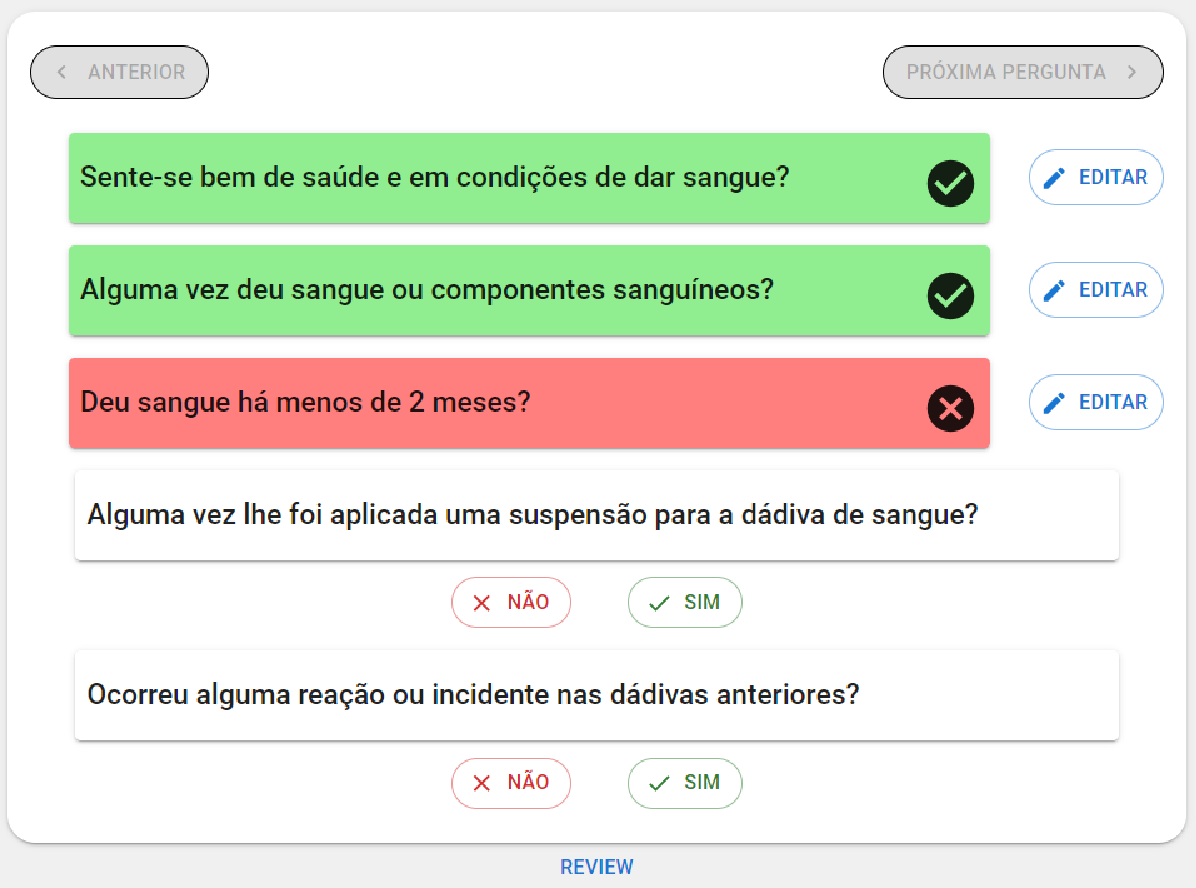
\includegraphics{./figures/Form3.pdf}}
	\end{center}
	\caption{Form Page with answers and no sub questions.}\label{fig:form3}
\end{figure}

\newpage

\subsection{EditFormPage \& useEditFormPage} \label{edit_form}
The EditFormPage component acts a an outlet for the backoffice component page. It leverages the useEditFormPage hook to retrieve the form structure from the backend and manage it's state.

As mentioned in Section \ref{arc_jre}, the type of form events in our system are:
\begin{itemize}
	\item \textbf{showQuestion:} show the question with id in the params field;
	\item \textbf{nextGroup:} allow for navigation to next group, is triggered when all the question in current group have been answered;
	\item \textbf{showReview:} allow form review, is triggered when all the answers in the form have been answered and donor can review form.
\end{itemize}

To generate the nextGroup event we iterate over all the group of questions and for each create a top level condition of the all type and then iterate over every question in that group to create more conditions within this top level condition.
These questions can be divided into two types, which generate different conditions:
\begin{itemize}
	\item \textbf{Independent questions:} These generate the simplest conditions, since they just need to have an answer;
	\item \textbf{Child questions:} If the question is a child of another question there are two possible scenarios, either the question is visible and it needs an answer or it isn't displayed and should be ignored. 
\end{itemize}

The first scenario generates a condition as illustrated in Listing \ref{independent_questions}.
\begin{lstlisting}[style=sharpc, caption={Condition generated by an independent questions}, label={independent_questions}]
conditions: {
	all: [
		{
			fact: 'IndependentQuestion1',
			operator: 'notEqual',
			value: ''
		},
		{
			fact: 'IndependentQuestion2',
			operator: 'notEqual',
			value: ''
		}
	],
}
\end{lstlisting}

Meanwhile the second scenario generates a condition as illustrated in Listing \ref{child_questions}, the all top level condition type is used as a question can have multiple parent questions.

\begin{lstlisting}[style=sharpc, caption={Condition generated by a child questions}, label={child_questions}]
	conditions: {
		all: [
			any: [
				{
					fact: 'ChildQuestion',
					operator: 'notEqual',
					value: ''
				},
				all:{
					fact: 'ParentQuestion',
					operator: 'notEqual',
					value: 'value that trigger child question display'
				}
			]
		],
	}
\end{lstlisting}


As the user edit's the form's structure the changes are reflected in the hook's state, which is specially difficult given that a question can be a parent, i.e. it's answer causes another question to appear, and a child, i.e. it appears as a result of another question's answer.

To solve this issue the hook can reassign questions upon deletion, by finding the group with the parent question and setting the show condition of it's child question as undefined, which means they're automatically shown.

A view of this component is illustrated in Figure \ref{fig:edit_form}.

\begin{figure}[h]
	\begin{center}
		\resizebox{160mm}{!}{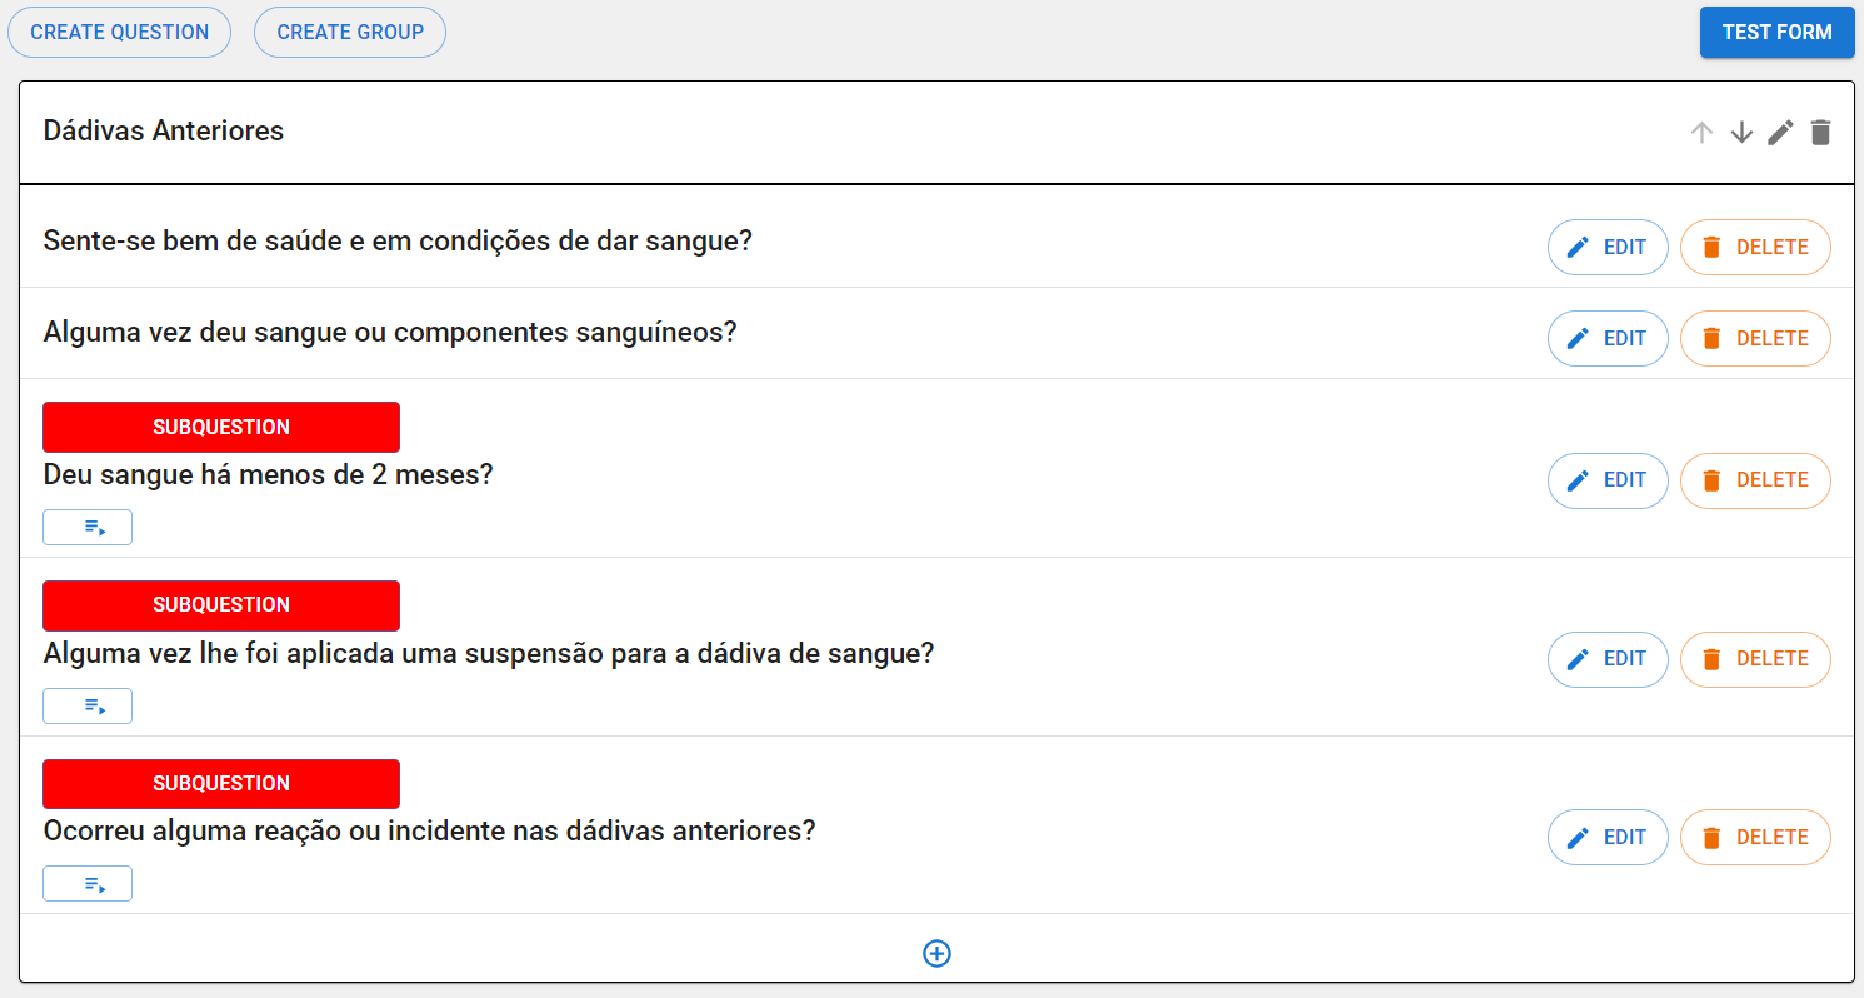
\includegraphics{./figures/Edit_Form.pdf}}
	\end{center}
	\caption{Form Page with answers and no sub questions.}\label{fig:edit_form}
\end{figure}

\subsection{EditTermsPage} \label{edit_terms}

The EditTermsPage component acts as an outlet for the backoffice component page. It provides an interface for editing the terms and conditions. This component leverages the Editor component, which integrates the Jodit WYSIWYG editor, offering a rich text editing experience. The state management is handled using the useEditTerms custom hook, which ensures seamless interaction with the backend.
The content of the editor is stored as HTML allowing for flexible presentation and formatting when displayed to end-users.

A view of this component is illustrated in Figure \ref{fig:edit_terms}.

\begin{figure}[h]
	\begin{center}
		\resizebox{160mm}{!}{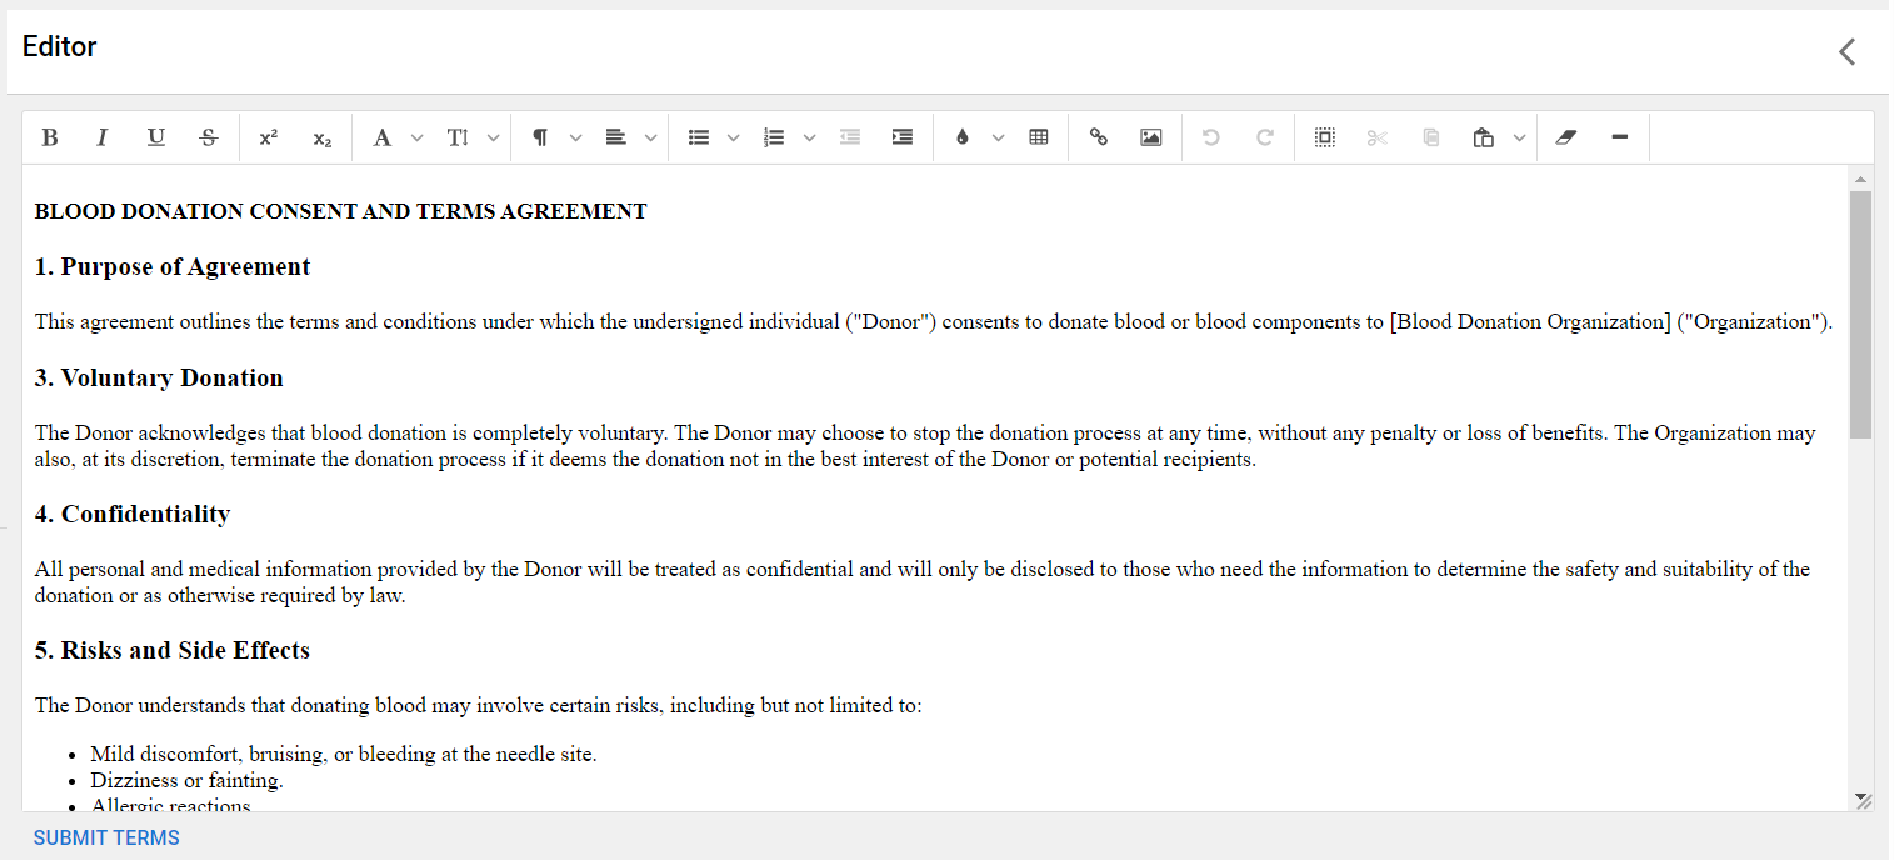
\includegraphics{./figures/Terms_Editor.pdf}}
	\end{center}
	\caption{Form Page with answers and no sub questions.}\label{fig:edit_terms}
\end{figure}

\newpage


\section{Role Based Access Control}
As previously mentioned, users are assigned one or more of the following roles: donor, doctor, or admin. Their actions and navigation within the platform are restricted based on their assigned role(s). Upon login, role claims are stored in a \textbf{JWT} (JSON Web Token) format within a cookie. By default, resource requests made to the backend include these credentials via the \textbf{credentials} option, where the credentials refer to the cookie with the JWT.

In addition to storing role claims in cookies, they are also saved in local storage to manage user navigation. While local storage is vulnerable to tampering, this is not a critical issue because sensitive data can only be accessed if the user possesses a valid JWT with the correct role claims. Since the JWT itself cannot be altered, security risks remain minimal.
\section{Navigation}

This chapter features a navigation graph, presented in Figure ~\ref{fig:userNavigation}, that describes the UI flow of our platform.
The primary entry point for all users is the Home page, from which navigation diverges based on the user's login status and role.
With admins being able to navigate throughout the platform, while doctors lack backoffice access and finally donors only having access to the terms and form page.

\begin{figure}[H]
	\begin{center}
		\resizebox{150mm}{!}{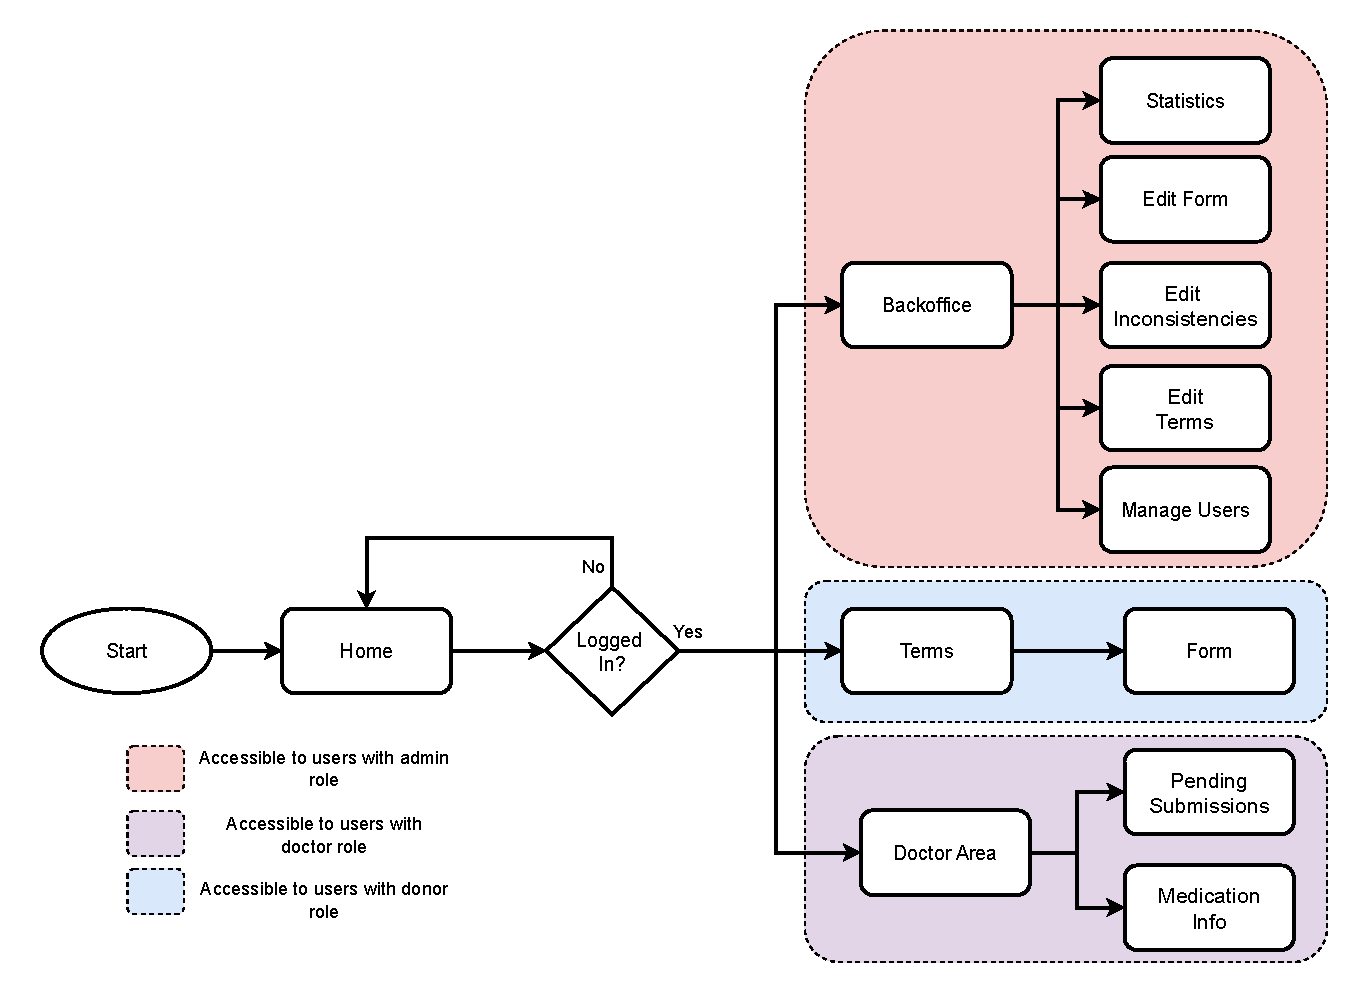
\includegraphics{./figures/userNavigation.pdf}}
	\end{center}
	\caption{UI navigation.}\label{fig:userNavigation}
\end{figure}



\section{Doctor Submission Review System and SSE}\label{SSE_frontend}

To keep the frontend updated with the real-time status of submissions (e.g., when they are locked or unlocked), the system uses Server-Sent Events (SSE). This connection allows the server to push updates to the client automatically, ensuring that doctors see the most current submission status without needing to refresh the page.

When a doctor enters the Pending Submissions page, the frontend sends a request to the /pending/notifications endpoint. This request registers the frontend as a notification client, establishing an SSE stream between the server and the client. Through this connection, the server can send real-time updates, such as lock and unlock events, to all connected clients.

This interaction works as follows:
\begin{itemize}
	\item \textbf{Locking:} When a doctor locks a submission, the system sends an SSE notification to all connected clients, notifying them that the submission is now locked and unavailable for review by others.
	\item \textbf{Unlocking:} When the doctor unlocks the submission or if the lock expires due to a timeout, an SSE notification is broadcasted, informing clients that the submission is now available.
	The frontend component (e.g., PendingSubmissions.tsx) listens for these SSE messages and updates the UI in real time to reflect the current status of submissions. This ensures doctors are always aware of which submissions are locked, preventing conflicts.
\end{itemize}












% Capitulo 6
%
% Capítulo 6
%
\chapter{Backend Implementation} \label{cap:backend_implementation}

The backend application is tasked with handling http requests, business logic and data persistence. 

The backend logic is implemented in C{\#} and data is persisted in a postgreSQL database, interaction with this database is done trough EF CORE.

An overview of the backend implementation is presented in Figure ~\ref{fig:backend_implementation}.
\begin{figure}[h]
	\begin{center}
		\resizebox{90mm}{!}{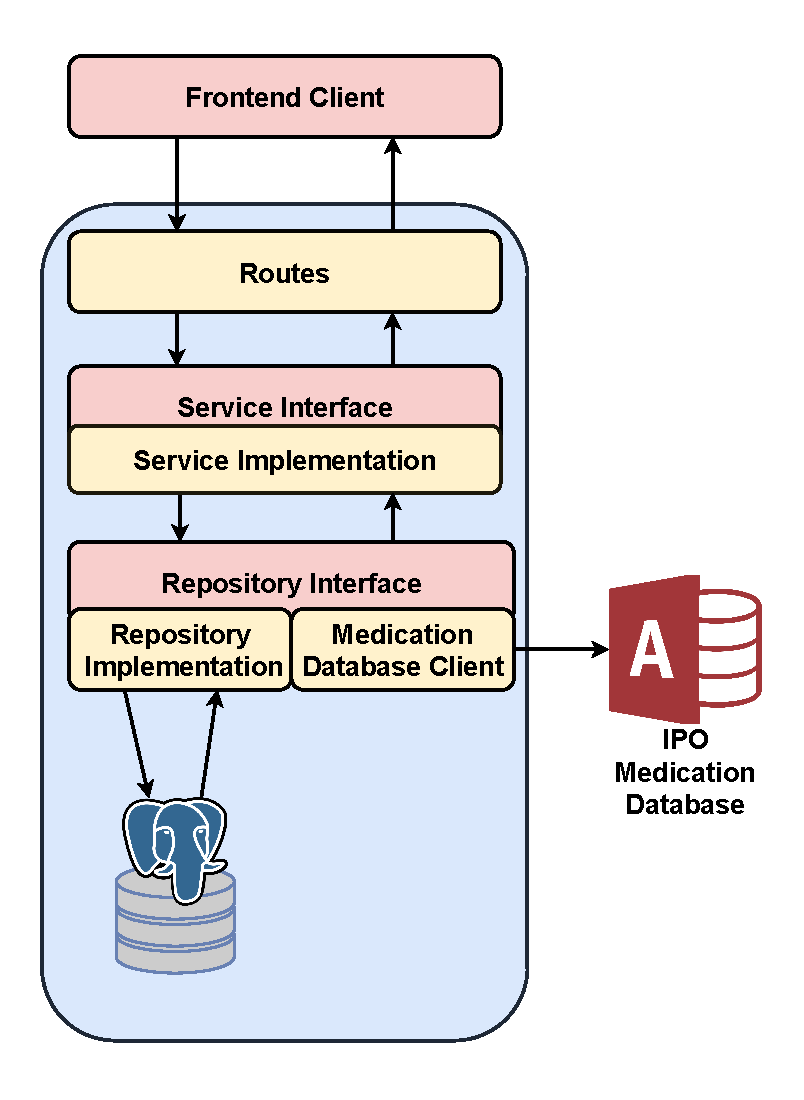
\includegraphics{./figures/backend_implementation.pdf}}
	\end{center}
	\caption{Block Diagram of our solution.}\label{fig:backend_implementation}
\end{figure}

\newpage

\section{Structure}

The structure for the backend application is as follows:

\begin{itemize}
	\item Program.cs: the entry point of the application;
	\item domain: contains all the domain classes;
	\item repositories: contains the backend repositories that communicate with the postgreSQL database;
	\begin{itemize}
		\item entities: contains the entities outlined in chapter \ref{cap:data_model}.
	\end{itemize}
	\item services: contains all the services that, validate and manipulate data, that is received or sent to the routes and repository layer;
	\item routes: contains all the routes of the API which call the adequate service.
	\item utils: contains auxiliary classes and methods.
\end{itemize}

\section{Program.cs}

The .NET framework makes use of a dependency injection container, aka the service container. As with the Spring Framework, dependencies can have various lifetimes, which in the .NET framework are as follows:
\begin{itemize}
	\item Transient: the dependency is created when needed and disposed thereafter;
	\item Scoped: the dependency is created and maintained in a per request basis;
	\item Singleton: once the dependency is created it's maintained throughout the application's lifetime. 
\end{itemize}
Beyond this, the framework also makes use of the builder pattern, meaning to build a web application we first instantiate a builder, i.e. a class that "knows" how to build a web application, and then supply the needed middlewares to build it, with the desired lifetime.
The aforementioned middlewares, which refer to the services and repositories, are registered as services in the container. In our application most of these services were registered with the Scoped scope, as illustrated in Listing \ref{DI}.

\begin{lstlisting}[style=sharpc, caption={Registering Scoped Services in ASP.NET Core Dependency Injection Container.}, label={DI}]
builder.Services.AddScoped<IUsersService, UsersService>();
builder.Services.AddScoped<IFormService, FormService>();
builder.Services.AddScoped<ITermsService, TermsService>();
builder.Services.AddScoped<IMedicationsService, MedicationsService>();
builder.Services.AddScoped<IManualService, ManualService>();
builder.Services.AddScoped<ISubmissionService, SubmissionService>();
builder.Services.AddScoped<IReviewsService, ReviewsService>();

builder.Services.AddScoped<IRepository, Repository>();
\end{lstlisting}

Using this registration method, for example, when a dependency of type IUsersService is needed, the service container creates a UsersService object to fufill that dependency, hence the inversion of control.

The services that don't make use of the scoped lifetime are associated with the lock management and server sent events, are illustrated in \ref{SSE_listing}, these services are elaborated on section \ref{label}.

\begin{lstlisting}[style=sharpc, caption={Registering Scoped Services in ASP.NET Core Dependency Injection Container:}, label={SSE_listing}]
builder.Services.AddSingleton<INotificationService, NotificationService>();
builder.Services.AddSingleton<NotificationEndpoint>();
builder.Services.AddHostedService<UnlockExpiredSubmissionsService>();

\end{lstlisting}

To allow for cross-origin resource sharing, i.e. to allow the frontend client to access the resources in the backend, we also had to create CORS policy, as follows:

\begin{lstlisting}[style=sharpc, caption={Configuring CORS Policy in ASP.NET Core: Allowing Specific Origin with Full Access Control.}]
builder.Services.AddCors(options =>
{
	options.AddPolicy("MyCorsPolicy",
	policy =>
	{
		policy.WithOrigins("http://localhost:8000")
		.AllowAnyHeader()
		.AllowAnyMethod()
		.AllowCredentials();
	});
});
\end{lstlisting}

Notice that request originating from port 8000 of the localhost ip can have any type of header, any HTTP method and can include credentials, such as cookies.
\newpage

\subsubsection{Authentication JWT}

Our platform uses JSON Web Tokens, \textbf{JWT} \cite{rfc7519}, to represent user claims.
These token's issuer, audience and key, refered to as jwtIssuer, jwtAudience and jwtKey in listing \ref{authentication} below, are stored in the appsettings.json file.

\begin{lstlisting}[style=sharpc, caption={Custom JWT Authentication Middleware in ASP.NET Core: Handling Unauthorized Access with Detailed Problem Responses.}, label={authentication}] 
builder.Services.AddAuthentication(x =>
{
	x.DefaultAuthenticateScheme = JwtBearerDefaults.AuthenticationScheme;
	x.DefaultChallengeScheme = JwtBearerDefaults.AuthenticationScheme;
}).AddJwtBearer(options =>
{
	options.Events = new JwtBearerEvents
	{
		...
		OnChallenge = context =>
		{
			context.HandleResponse();
			
			context.Response.ContentType = "application/problem+json";
			context.Response.StatusCode = StatusCodes.Status401Unauthorized;
			var problemDetails = new
			{
				type = "https://localhost:8000/errors/unauthorized",
				title = "Unauthorized",
				detail = "You are not authorized to access this resource. Please provide valid credentials.",
				status = StatusCodes.Status401Unauthorized
			};
			var problemJson = JsonSerializer.Serialize(problemDetails);
			return context.Response.WriteAsync(problemJson);
		}
	};
	options.SaveToken = true;
	options.TokenValidationParameters = new TokenValidationParameters
	{
		ValidateIssuer = true,
		ValidateAudience = true,
		ValidateLifetime = true,
		ValidateIssuerSigningKey = true,
		ValidIssuer = jwtIssuer,
		ValidAudience = jwtAudience,
		IssuerSigningKey = new SymmetricSecurityKey(Encoding.UTF8.GetBytes(jwtKey))
	};
});
\end{lstlisting}

Notice that in case the \textbf{JWT} isn't valid the default behavior of responding with a 401 status code and an empty body is suppressed by "context.HandleResponse()" and instead a Problem response is sent with more details.

\subsubsection{Role Based Access Control}
In our system, users are assigned one of three roles: donor, doctor, or admin. Each of these roles grants access to a specific set of endpoints, ensuring that users can only interact with the parts of the application that are relevant to their role. To enforce this, we have configured authorization policies within the ASP.NET Core framework, which restrict access based on the role claims present in the user's JSON Web Token (JWT).

As shown in Listing \ref{rbac}, we define three authorization policies—one for each role. The AddAuthorization method is used to add these policies to the service container. Each policy requires that the user’s JWT contains a claim of type ClaimTypes.Role with a corresponding value of either donor, doctor", or admin.

\begin{lstlisting}[style=sharpc, caption={Configuring Role-Based Authorization Policies in ASP.NET Core: Defining Access Control for Donor, Doctor, and Admin Roles.}, label={rbac}] 
builder.Services.AddAuthorization(options =>
{
	options.AddPolicy("donor", policy => policy.RequireClaim(ClaimTypes.Role, "donor"));
	options.AddPolicy("doctor", policy => policy.RequireClaim(ClaimTypes.Role, "doctor"));
	options.AddPolicy("admin", policy => policy.RequireClaim(ClaimTypes.Role, "admin"));
});
\end{lstlisting}

When defining an endpoint, we can specify which authorization policy should be applied. For instance, an endpoint that should only be accessible to doctors can be protected by the "doctor" policy.

By leveraging these role-based authorization policies, we enforce a clear and secure access control mechanism, ensuring that users can only perform actions that are appropriate for their role. This approach not only enhances security but also simplifies the management of user permissions across the application.

%Beyond these, we also used an ElasticClient, however in this service registration, we use a different pattern, instead of using a type and implementation, only the latter was used, this method doesn't allow for multiple implementation, but since there was no need to mock the elastic search database, this feature wasn't needed.
%
%\begin{lstlisting}[style=sharpc]
%var nodePool = new SingleNodePool(new Uri("http://localhost:9200"));
%var settings = new ElasticsearchClientSettings(
% nodePool,
% sourceSerializer: (_, settings) =>
%  {
	%    return new DefaultSourceSerializer(settings, options =>
	%      {
		%        options.Converters.Add(new AnswerConverter());
		%        options.Converters.Add(new ConditionConverter());
		%      });
	%  });
%builder.Services.AddSingleton(new ElasticsearchClient(settings));
%\end{lstlisting}
%
%According to the Elastic Search documentation, as long as the client instance is a singleton, our application database is thread safe.
\newpage
\subsection{Repositories}

The Repository layer acts as a vital intermediary for data access within the application. It ensures the database and service layer remain independent from one another. This separation allows the service layer to access data without being tightly coupled to the database, facilitating easy database switching by merely replacing this module.

By defining a well-known interface contract, we can abstract the implementation details.

Utilizing a transaction manager in the service layer enables our solution to handle multiple concurrent accesses across various resources and provides rollback capabilities for effective error handling.

%The main idea in the repositories is to allow for CRUD operations, ie create users/forms, read users/forms, update users/forms and delete users/forms, on data that is or will be stored in an Elastic Search database. As such the repositories have a dependency on the ElasticsearchClient mentioned before, and they'll use the same client but target different indexes.

\subsubsection{Form Repository}

The form repository is responsible for the Form, Submission, Review, Inconsistency entities.

And this repository will have the following methods:

\begin{lstlisting}[style=sharpc]
	public interface IFormRepository
	{
		public Task<Form> GetForm();
		
		public Task<Form?> GetFormWithVersion(int version);
		
		public Task<Form> EditForm(Form form);
		
		public Task<bool> SubmitForm(Submission submission);
		
		public Task<List<Submission>?> GetPendingSubmissions();
		
		public Task<Submission> GetSubmission(int nic);
		
		public Task<Submission?> GetSubmissionById(int id);
		
		public Task<Submission?> GetLatestPendingSubmissionByUser(int userNic);
		
		public Task<(List<SubmissionHistoryDto>? Submissions, bool HasMoreSubmissions)> GetSubmissionHistoryByNic(int nic, int limit, int skip);
		
		public Task<Inconsistencies> GetInconsistencies();
		
		public Task<bool> LockSubmission(int submissionId, int doctorId);
		
		public Task<bool> UnlockSubmission(int submissionId, int doctorId);
		
		public Task<List<SubmissionLock>> GetExpiredLocks(TimeSpan timeout);
		
		public Task<bool> SubmissionExists(int id);
		
		public Task<Review> AddReview(Review review);
		
		public Task<bool> AddNote(Note note);
		
		public Task<bool> EditInconsistencies(Inconsistencies inconsistencies);
	}
\end{lstlisting}

\subsubsection{User Repository}

The user repository will be responsible for the User, UserAccountStatus and UserSuspension entities

And this repository will have the following methods:
\begin{lstlisting}[style=sharpc]
	public interface IUsersRepository
	{
		public Task<bool> AddUser(User user);
		
		public Task<List<User>?> GetUsers();
		
		public Task<User?> GetUserByNic(int nic);
		
		public Task<Boolean> DeleteUser(int nic);
		
		public Task<UserAccountStatus?> GetUserAccountStatus(int userNic);
		
		public Task<Boolean> UpdateUserAccountStatus(UserAccountStatus userAccountStatus);
		
		public Task<bool> AddSuspension(UserSuspension suspension);
		public Task<bool> UpdateSuspension(UserSuspension suspension);
		public Task<UserSuspension?> GetSuspension(int userNic);
		public Task<bool> DeleteSuspension(int userNic);
		
	}
\end{lstlisting}

\newpage

\subsection{Services}
Each service is responsible for managing a certain group of requests, i.e. the logic to fulfill a request to the /users endpoint will be in the user services. Each service as a dependency on their corresponding repository, which is handled by the service container.

The methods within each service will reflect the possible actions outlined in Chapter ~\ref{cap:problem_description}'s section on uses cases.

\subsubsection{Error Handling Implementation}
As mentioned in section \ref{service_layer_error_handling} we will utilize a \textbf{Result} class which can encapsulate either a successful outcome or an error.

To enforce this practice, every service method returns a Result, and each service call in the route layer is wrapped by a HandleRequest method. This method belongs to the HttpExtensions class, as illustrated in Listing \ref{HttpExtensions}.

\begin{lstlisting}[style=sharpc, caption={Custom Extension Methods for Handling HTTP Requests in ASP.NET Core: Simplifying Success and Error Response Handling.}, label={HttpExtensions}]
public static class HttpExtensions
{
	public static IResult HandleRequest<TIn>(
	this Result<TIn> result, Func<TIn,IResult> onSuccess)
	{
		return result.IsSuccess ? onSuccess(result.Value) : Results.Problem(ErrorToProblem(result.Errors[0]));
	}
	
	public static IResult HandleRequest(
	this Result result, Func<IResult> onSuccess)
	{
		return result.IsSuccess ? onSuccess() : Results.Problem(ErrorToProblem(result.Errors[0]));
	}
	
	private static ProblemDetails ErrorToProblem(IError error)
	{
		Console.Out.WriteLine("Error:" + error);
		return new ProblemDetails();
	}
}
\end{lstlisting}


The HandleRequest method is an extension method designed to streamline the handling of HTTP requests by automatically processing the result of a service call.

The first HandleRequest method, defined on lines 3-7, handles cases where the service call returns a value. If the operation is successful (IsSuccess is true), it invokes the onSuccess function, passing the successful result value (result.Value) to generate the appropriate HTTP response. If the operation fails, it calls the Results.Problem method to generate a standardized error response, using the first error in the Errors collection to populate the ProblemDetails object.

Similarly, the second HandleRequest method, defined on lines 9-13, handles cases where the service method returns a Result without a value. It follows the same logic: if the operation is successful, it executes the onSuccess function to produce the HTTP response; otherwise, it generates a ProblemDetails response to represent the error.

The private ErrorToProblem method (lines 15-19) converts an IError object into a ProblemDetails object. This method is responsible for translating internal error details into a standardized format that can be returned as part of an HTTP problem response. The method currently includes a line to output the error details to the console for debugging purposes.

By employing these extension methods, we simplify the process of handling success and error scenarios across the entire application. This ensures that all HTTP responses are consistent, well-structured, and easy to manage, which enhances both the maintainability and reliability of the codebase.

\subsubsection{User Service}

\begin{lstlisting}[style=sharpc]
	public interface IUsersService
	{
		public Task<Result<Token, Problem>> CreateToken(int nic, string password);
		
		public Task<Result<UserExternalInfo, Problem>> CreateUser(int nic, string name, string password, Role role);
		
		public Task<Result<List<UserExternalInfo>, Problem>> GetUsers(string token);
		
		public Task<Result<Boolean, Problem>> DeleteUser(int nic);
		
		public Task<Result<UserAccountStatus?, Problem>> GetUserAccountStatus(int userNic);
		
		public Task<Result<Boolean, Problem>> UpdateUserAccountStatus(UserAccountStatus userAccountStatus);
		
		public Task<Result<UserWithNameExternalInfo?, Problem>> CheckNicExistence(int nic);
		
		public Task<Result<bool, Problem>> AddSuspension(UserSuspensionRequest suspension);
		
		public Task<Result<bool, Problem>> UpdateSuspension(UserSuspension suspension);
		
		public Task<Result<UserSuspension?, Problem>> GetSuspension(int userNic);
		
		public Task<Result<bool, Problem>> DeleteSuspension(int userNic);
	}
\end{lstlisting}

\newpage

\subsubsection{Terms Service}

\begin{lstlisting}[style=sharpc]
	public interface ITermsService
	{
		public Task<Result<List<Terms>, Problem>> GetTerms();
		public Task<Result<Terms, Problem>> GetActiveTerms();
		public Task<Result<bool, Problem>> SubmitTerms(Terms terms);
		
		public Task<Result<bool, Problem>> UpdateTerms(int termId, int updatedBy, string newContent);
		
		public Task<Result<List<TermsChangeLog>?, Problem>> GetTermsChangeLog(int termId);
	}
\end{lstlisting}


\subsubsection{Form Service}

\begin{lstlisting}[style=sharpc]
	public interface IFormService
	{
		public Task<Result<GetFormOutputModel, Problem>> GetForm();
		
		public Task<Result<GetFormWithVersionOutputModel, Problem>> GetFormWithVersion(int version);
		
		public Task<Result<Form, Problem>> EditForm(List<QuestionGroupModel> groups, List<RuleModel> rules, User user);
		
		public Task<Result<SubmitFormOutputModel, Problem>> SubmitForm(Dictionary<string,IAnswer> answers, int nic, int formVersion);
		
		public Task<Result<Submission, Problem>> GetSubmission(int id);
		
		public Task<Result<bool, Problem>> LockSubmission(int submissionId, int doctorId);
		
		public Task<Result<bool, Problem>> UnlockSubmission(int submissionId, int doctorId);
		
		public Task UnlockExpiredSubmissions(TimeSpan lockTimeout);
		
		public Task<Result<Review, Problem>> ReviewForm(int submissionId, int doctorNic, string status, string? finalNote, List<NoteModel>? noteModels = null);
		
		public Task<Result<List<Submission>, Problem>> GetPendingSubmissions();
		
		public Task<Result<Inconsistencies, Problem>> GetInconsistencies();
		
		public Task<Result<Submission?, Problem>> GetPendingSubmissionsByUserNic(int userNic);
		
		public Task<Result<SubmissionHistoryOutputModel, Problem>> GetSubmissionHistoryByNic(int nic, int limit, int skip);
		
		public Task<Result<bool, Problem>> EditInconsistencies(Inconsistencies inconsistencies);
	}
\end{lstlisting}


\subsubsection{Manual Service}

\begin{lstlisting}[style=sharpc]
	public interface IManualService
	{
		public Task<Result<List<ManualInformation>, Problem>> GetManualInformation(string productName);
	}
\end{lstlisting}


\subsubsection{Medication Service}

\begin{lstlisting}[style=sharpc]
	public interface IMedicationsService
	{
		Task<Result<List<string>, Problem>> SearchMedications(string query);
	}
\end{lstlisting}

\newpage

\subsection{Routes}

\subsubsection{User Routes}
The available endpoints, HTTP method and corresponding operation for all the user routes are available in Table ~\ref{tab:user_endpoints}. 

\begin{table}[h!]
	\begin{center}
		\begin{tabular}{l|c|l} 
			\textbf{Endpoint} & \textbf{HTTP Method} & \textbf{Description} \\
			\hline
			/users & POST & \makecell{Creates a new user} \\
			\hline
			/users & GET & \makecell{Retrieves all users} \\
			\hline
			/users/\{nic\} & GET & \makecell{Checks the existence of a user with the specified NIC}\\
			\hline
			/users/\{nic\} & DELETE & \makecell{Deletes the user with the specified NIC} \\
			\hline
			/users/login & POST & \makecell{Creates a new access token} \\
			\hline
			/users/status/\{nic\} & GET & \makecell{Retrieves the status of the user account\\ with the specified NIC} \\
			\hline
			/update-status & POST & \makecell{Updates the status of a user account} \\
			\hline
			/users/suspension & POST & \makecell{Adds a new suspension} \\
			\hline
			/users/suspension/update & POST & \makecell{Updates an existing suspension} \\
			\hline
			/users/suspension/\{nic\} & GET & \makecell{Retrieves the suspension details for the specified NIC} \\
			\hline
			/users/suspension/\{nic\} & DELETE & \makecell{Deletes the suspension for the specified NIC} \\
		\end{tabular}
		
		\caption{API endpoints related to the user}\label{tab:user_endpoints}
	\end{center}
\end{table}

\subsubsection{Form Routes}
The available endpoints, HTTP method and corresponding operation for all the form routes are available in Table ~\ref{tab:form_endpoints}. 

\begin{table}[h!]
	\begin{center}
		\begin{tabular}{l|c|l} 
			\textbf{Endpoint} & \textbf{HTTP Method} & \textbf{Description} \\
			\hline
			/forms/structure & GET & \makecell{Retrieves the form structure} \\
			\hline
			/forms/structure & PUT & \makecell{Edits the form structure} \\
			\hline
			/forms/structure/\{version:int\} & GET & \makecell{Retrieves the form structure \\ for the specified version} \\
			\hline
			/forms/submissions & GET & \makecell{Retrieves pending submissions} \\
			\hline
			/forms/submissions/\{nic:int\} & POST & \makecell{Submits a form} \\
			\hline
			/forms/submissions/\{nic:int\} & GET & \makecell{Retrieves a pending submission \\ for the specified NIC} \\
			\hline
			/forms/submissions/history/\{nic:int\} & GET & \makecell{Retrieves submission history \\ for the specified NIC} \\
			\hline
			/forms/submissions/\{submissionId:int\}/lock & POST & \makecell{Locks a submission} \\
			\hline
			/forms/submissions/\{submissionId:int\}/unlock & POST & \makecell{Unlocks a submission} \\
			\hline
			/forms/inconsistencies & GET & \makecell{Retrieves inconsistencies} \\
			\hline
			/forms/inconsistencies & PUT & \makecell{Edits inconsistencies} \\
			\hline
			/forms/review/\{submissionId:int\} & POST & \makecell{Reviews a form submission} \\
			\hline
			/forms/notifications & GET & \makecell{Sets up server-sent \\ event notifications} \\
		\end{tabular}
		
		\caption{API endpoints related to the form}\label{tab:form_endpoints}
	\end{center}
\end{table}

\subsubsection{Terms Routes}
\begin{table}[h!]
	\begin{center}
		\begin{tabular}{l|c|l} 
			\textbf{Endpoint} & \textbf{HTTP Method} & \textbf{Description} \\
			\hline
			/terms & GET & \makecell{Retrieves all the terms} \\
			\hline
			/terms/active & GET & \makecell{Retrieves the active terms} \\
			\hline
			/terms & POST & \makecell{Submits terms} \\
			\hline
			/terms/\{termsId:int\} & PUT & \makecell{Updates terms with the specified termsId} \\
			\hline
			/terms/change-log/\{termsId:int\} & GET & \makecell{Gets the change-logs\\ for the terms with  specified termsId} \\
		\end{tabular}
		
		\caption{API endpoints related to the form}\label{tab:term_endpoints}
	\end{center}
\end{table}

\subsubsection{Medication and Manual Routes}
\begin{table}[h!]
	\begin{center}
		\begin{tabular}{l|c|l} 
			\textbf{Endpoint} & \textbf{HTTP Method} & \textbf{Description} \\
			\hline
			/medications/search & GET & \makecell{Retrieves medication list according to a query string} \\
			\hline
			/manual/\{product:string\} & GET & \makecell{Retrieves the blood donation information relevant to the specific product} \\
		\end{tabular}
		
		\caption{API endpoints related to the form}\label{tab:medication_manual_endpoints}
	\end{center}
\end{table}

\section{Password Security}\label{sec:security}

Two common password attacks are brute force attacks, and side-channel attacks.

Brute force attacks leverage the high computational power of Graphics Processing Units (GPUs) to paralelize password hashing tasks.

Side-channel attacks try get indirect information leaked during the execution of cryptographic algorithms, ie the time or power it takes for a system to hash a password.

\subsection{Mitigation}

Password hashing is a crucial security measure used to protect stored passwords. Instead of saving passwords in plaintext, which can be easily compromised, passwords are transformed into a hashed format using a hashing algorithm.

The work factor is the number of iterations of the hashing algorithm that are performed for each password. The work factor is typically stored in the hash output. It makes calculating the hash more computationally expensive, which in turn reduces the speed and/or increases the cost for which an attacker can attempt to crack the password hash \cite{owasp_password_storage}, which increases the brute-force attack further.
Choosing a work factor requires a compromise between security and performance, since, if to much computing power is required to hash a password the system becomes targetable to denial of service attacks.

Hashing algorithms that employ constant time operations and parallelism whenever possible help mitigate the risk of side channel attacks, as these factors increases the difficulty to extract information form side-channels.  


\subsection{Argon2id}
Argon2\cite{rfc9106} is a state-of-the-art password hashing algorithm that won the Password Hashing Competition in 2015. It comes in three variants: Argon2d, Argon2i, and Argon2id. Argon2id is a hybrid version that combines the benefits of both Argon2d (which provides resistance against brute-force attacks) and Argon2i (which is designed for side-channel attack resistance), and will be the algorithm used to secure the passwords for our platform.

Argon2id takes in configurable parameter, such as:
\begin{itemize}
	\item \textbf{Memory Cost}: The amount of memory (in kilobytes) used by the algorithm;
	\item \textbf{Time Cost} : The number of iterations the algorithm runs, which affects the computation time;
	\item \textbf{Parallelism} : The number of parallel threads used to process the hash.
\end{itemize}

Since these parameters are configurable it is possible to adjust them throughout the lifetime of an application, for example increase the time cost as the hosting hardware's capacity increases, and decrease it if concurrent accesses increase.

\newpage

\section{Testing}

Testing is a crucial step in ensuring the reliability and functionality of our application. This chapter outlines the approaches and tools used to validate the correctness of our code.

\subsection{Manual Testing}

During the development of the application, particularly on the backend, manual testing was employed to verify that the system behaved as expected. The primary tools used for manual testing were:

\begin{itemize} 
	\item \textbf{Swagger:} Swagger was utilized to test the API through HTTP requests. Although Swagger is primarily an API documentation and automation tool, it provides the necessary features for effective manual testing of APIs. 
	\item \textbf{Postman:} Postman was occasionally used to interact with ElasticSearch, specifically for data retrieval and storage operations. 
\end{itemize}

\subsection{Programmatic Testing}
Programmatic testing involves the use of specialized software tools to ensure the correctness and robustness of the application. This approach allows for repetitive and comprehensive testing of the codebase, improving efficiency and coverage.

\subsubsection{Unit Tests}
Unit tests are designed to verify the behavior of individual components or modules in isolation. We followed the Arrange-Act-Assert (AAA) pattern to structure our unit tests:

\begin{itemize} 
	\item \textbf{Arrange:} Prepare the necessary preconditions and inputs for the test. 
	\item \textbf{Act:} Execute the operation or function being tested. 
	\item \textbf{Assert:} Verify that the outcome matches the expected result. 
\end{itemize}

We employed xUnit.net, a free and open-source unit testing tool for the .NET framework, to execute our unit tests.

\subsubsection{Integration Tests}

TODO


% Capitulo 6
%\chapter{Project's current state} \label{cap:state}

The solution currently offers functionalities to:
\begin{itemize}
	\item Register and login users.
	
	\item Fill out a digital pre-donation form, that encompasses both the main questions of the form as well as relevant follow-up questions, that are triggered according to the user's responses.
	
	\item Manage the form's questions as well as the form's rules and manage users.
\end{itemize}

The project is currently experiencing some delays. These setbacks are primarily due to the inherent complexity of the project and our lack of knowledge in this particular domain.

One of the significant hurdles we have faced is the development of the backoffice's UI. Creating an intuitive and simple visual representation of both the form's questions and the underlying rules has proven to be particularly difficult. Ensuring that the user interface is both user-friendly and accurately reflects the complexity of the rules involved has required substantial effort and ongoing iterative refinement.

Furthermore, we remain committed to delivering a solution that will automatically verify drug and pathology interactions with blood donations. Although this feature is optional, it has the potential to significantly enhance the blood donation procedure. However, the lack of easily accessible, machine-readable information from the IPST manual has posed a significant challenge. Extracting and integrating this critical data in a way that ensures accuracy and reliability has been a complex task.


% Capitulo 7
%\chapter{Tests} \label{cap:tests}

Testing is a crucial step in ensuring the reliability and functionality of our application. This chapter outlines the approaches and tools used to validate the correctness of our code.

\section{Manual Testing}

During the development of the application, particularly on the backend, manual testing was employed to verify that the system behaved as expected. The primary tools used for manual testing were:

\begin{itemize} 
	\item \textbf{Swagger:} Swagger was utilized to test the API through HTTP requests. Although Swagger is primarily an API documentation and automation tool, it provides the necessary features for effective manual testing of APIs. 
	\item \textbf{Postman:} Postman was occasionally used to interact with ElasticSearch, specifically for data retrieval and storage operations. 
\end{itemize}

\section{Programmatic Testing}
Programmatic testing involves the use of specialized software tools to ensure the correctness and robustness of the application. This approach allows for repetitive and comprehensive testing of the codebase, improving efficiency and coverage.

\subsection{Unit Tests}
Unit tests are designed to verify the behavior of individual components or modules in isolation. We followed the Arrange-Act-Assert (AAA) pattern to structure our unit tests:

\begin{itemize} 
	\item \textbf{Arrange:} Prepare the necessary preconditions and inputs for the test. 
	\item \textbf{Act:} Execute the operation or function being tested. 
	\item \textbf{Assert:} Verify that the outcome matches the expected result. 
\end{itemize}

We employed xUnit.net, a free and open-source unit testing tool for the .NET framework, to execute our unit tests.

\subsection{Integration Tests}

TODO

% Capitulo 7
\chapter{Conclusions and Future Work} \label{cap:future}
In the final chapter of this report, we will summarize the accomplishments of this project, discuss the challenges encountered, and outline potential improvements and features that were envisioned but not implemented due to time constraints.
\section{Accomplishments}

In the introduction of this report, we outlined the current state of blood donation in Portugal, emphasizing the concerning decline in both donors and donations. We identified a platform with the potential to not only improve donor participation but also simplify the screening process for healthcare professionals.

A notable achievement was the development of functionalities that allow for the display and editing of form structures and rules as detailed in this document. These features are not limited to a specific domain, making the solution versatile and capable of being applied to various other challenges.

\section{Challenges}
The biggest challenge we faced in this project stemmed from our lack of experience in three critical areas: working with clients, defining project scopes, and estimating timelines.

Interacting with clients can be particularly challenging, especially when one lacks both general experience and specific knowledge of the domain. Understanding client needs, managing expectations, and maintaining clear communication proved difficult due to this inexperience. As a result, the project scope remained somewhat unclear and continued to evolve throughout development. This led us to stray from a more focused approach on delivering a smaller set of essential functionalities.

Additionally, our unfamiliarity with the .NET framework and the use of a rules engine made it difficult to accurately estimate how much time would be needed to develop an effective solution. This lack of technical familiarity further compounded the challenges of project planning and execution.




\section{Future Work}
The IPST medication guideline are organized in a table like manner, in the following column layout:
\begin{enumerate}
	\item Class/Group of Medication: This column categorizes medications.
	\item Active Substance/Commercial Name: This column lists either the active ingredient or the brand name of the medication.
	\item Criteria: This column specifies if a particular class or group of medications affects eligibility for blood donation, including details such as the duration of ineligibility and other relevant conditions.
\end{enumerate}
The terms used in the first column are, from what we can access, similar to the available pharmacotherapeutic classifications. A reliable source of a drug's pharmacotherapeutic classification is a portal provided by Infarmed\cite{CITS} to it's partner organizations, such as Lisbon's IPO.
As such, upon a donor's form submission, assuming they were taking some medication, our application would perform requests to said portal, get the appropriate pharmacotherapeutic classification and, by cross-checking the classification with the term used in the first column of the guidelines, return the relevant interaction information.
However, the terms used in the guidelines don't always reflect the available classifications, and, as such, the platform would need to employ some form of automated categorization, and allow for manual manipulation of these associations by the administrators.

It would also be a valuable feature to have the platform automatically check if the donor had any vaccinations and/or prescriptions that could be medically relevant. It would require integration with the SNS, and/or Infarmed systems.

\section{Acknowledgements}

We would like to extend our heartfelt gratitude to our supervisors, whose guidance and expertise have been instrumental throughout this project. Their support has been invaluable in shaping our approach and overcoming the challenges we faced. Additionally, we would like to express our sincere thanks to the staff at the Instituto Português de Oncologia (IPO) in Lisbon for their collaboration and insights, with a special thanks to Dr. Luís Ribeiro who allowed us to follow along with real time blood donations to give us a complete understanding of the procedure. Their contributions and feedback were essential in ensuring that the platform aligns with real-world needs and healthcare standards. This project would not have been possible without the collective efforts of everyone involved.

% Referências
\bibliographystyle{unsrt}
\bibliography{referencias}
\addcontentsline{toc}{chapter}{Refer\^{e}ncias}

% Apêndices (opcional)
\appendix
\chapter{ER MODEL}\label{er}

\begin{figure}[H]
	\begin{center}
		\rotatebox[origin=c]{90}{\includegraphics[width=\textwidth,height=\textheight,keepaspectratio]{./figures/ER_Model2.pdf}}
	\end{center}
	\caption{ER Model.}
\end{figure}



\chapter{Mocks}\label{mocks}

\begin{figure}[h]
	\begin{center}
		\resizebox{160mm}{!}{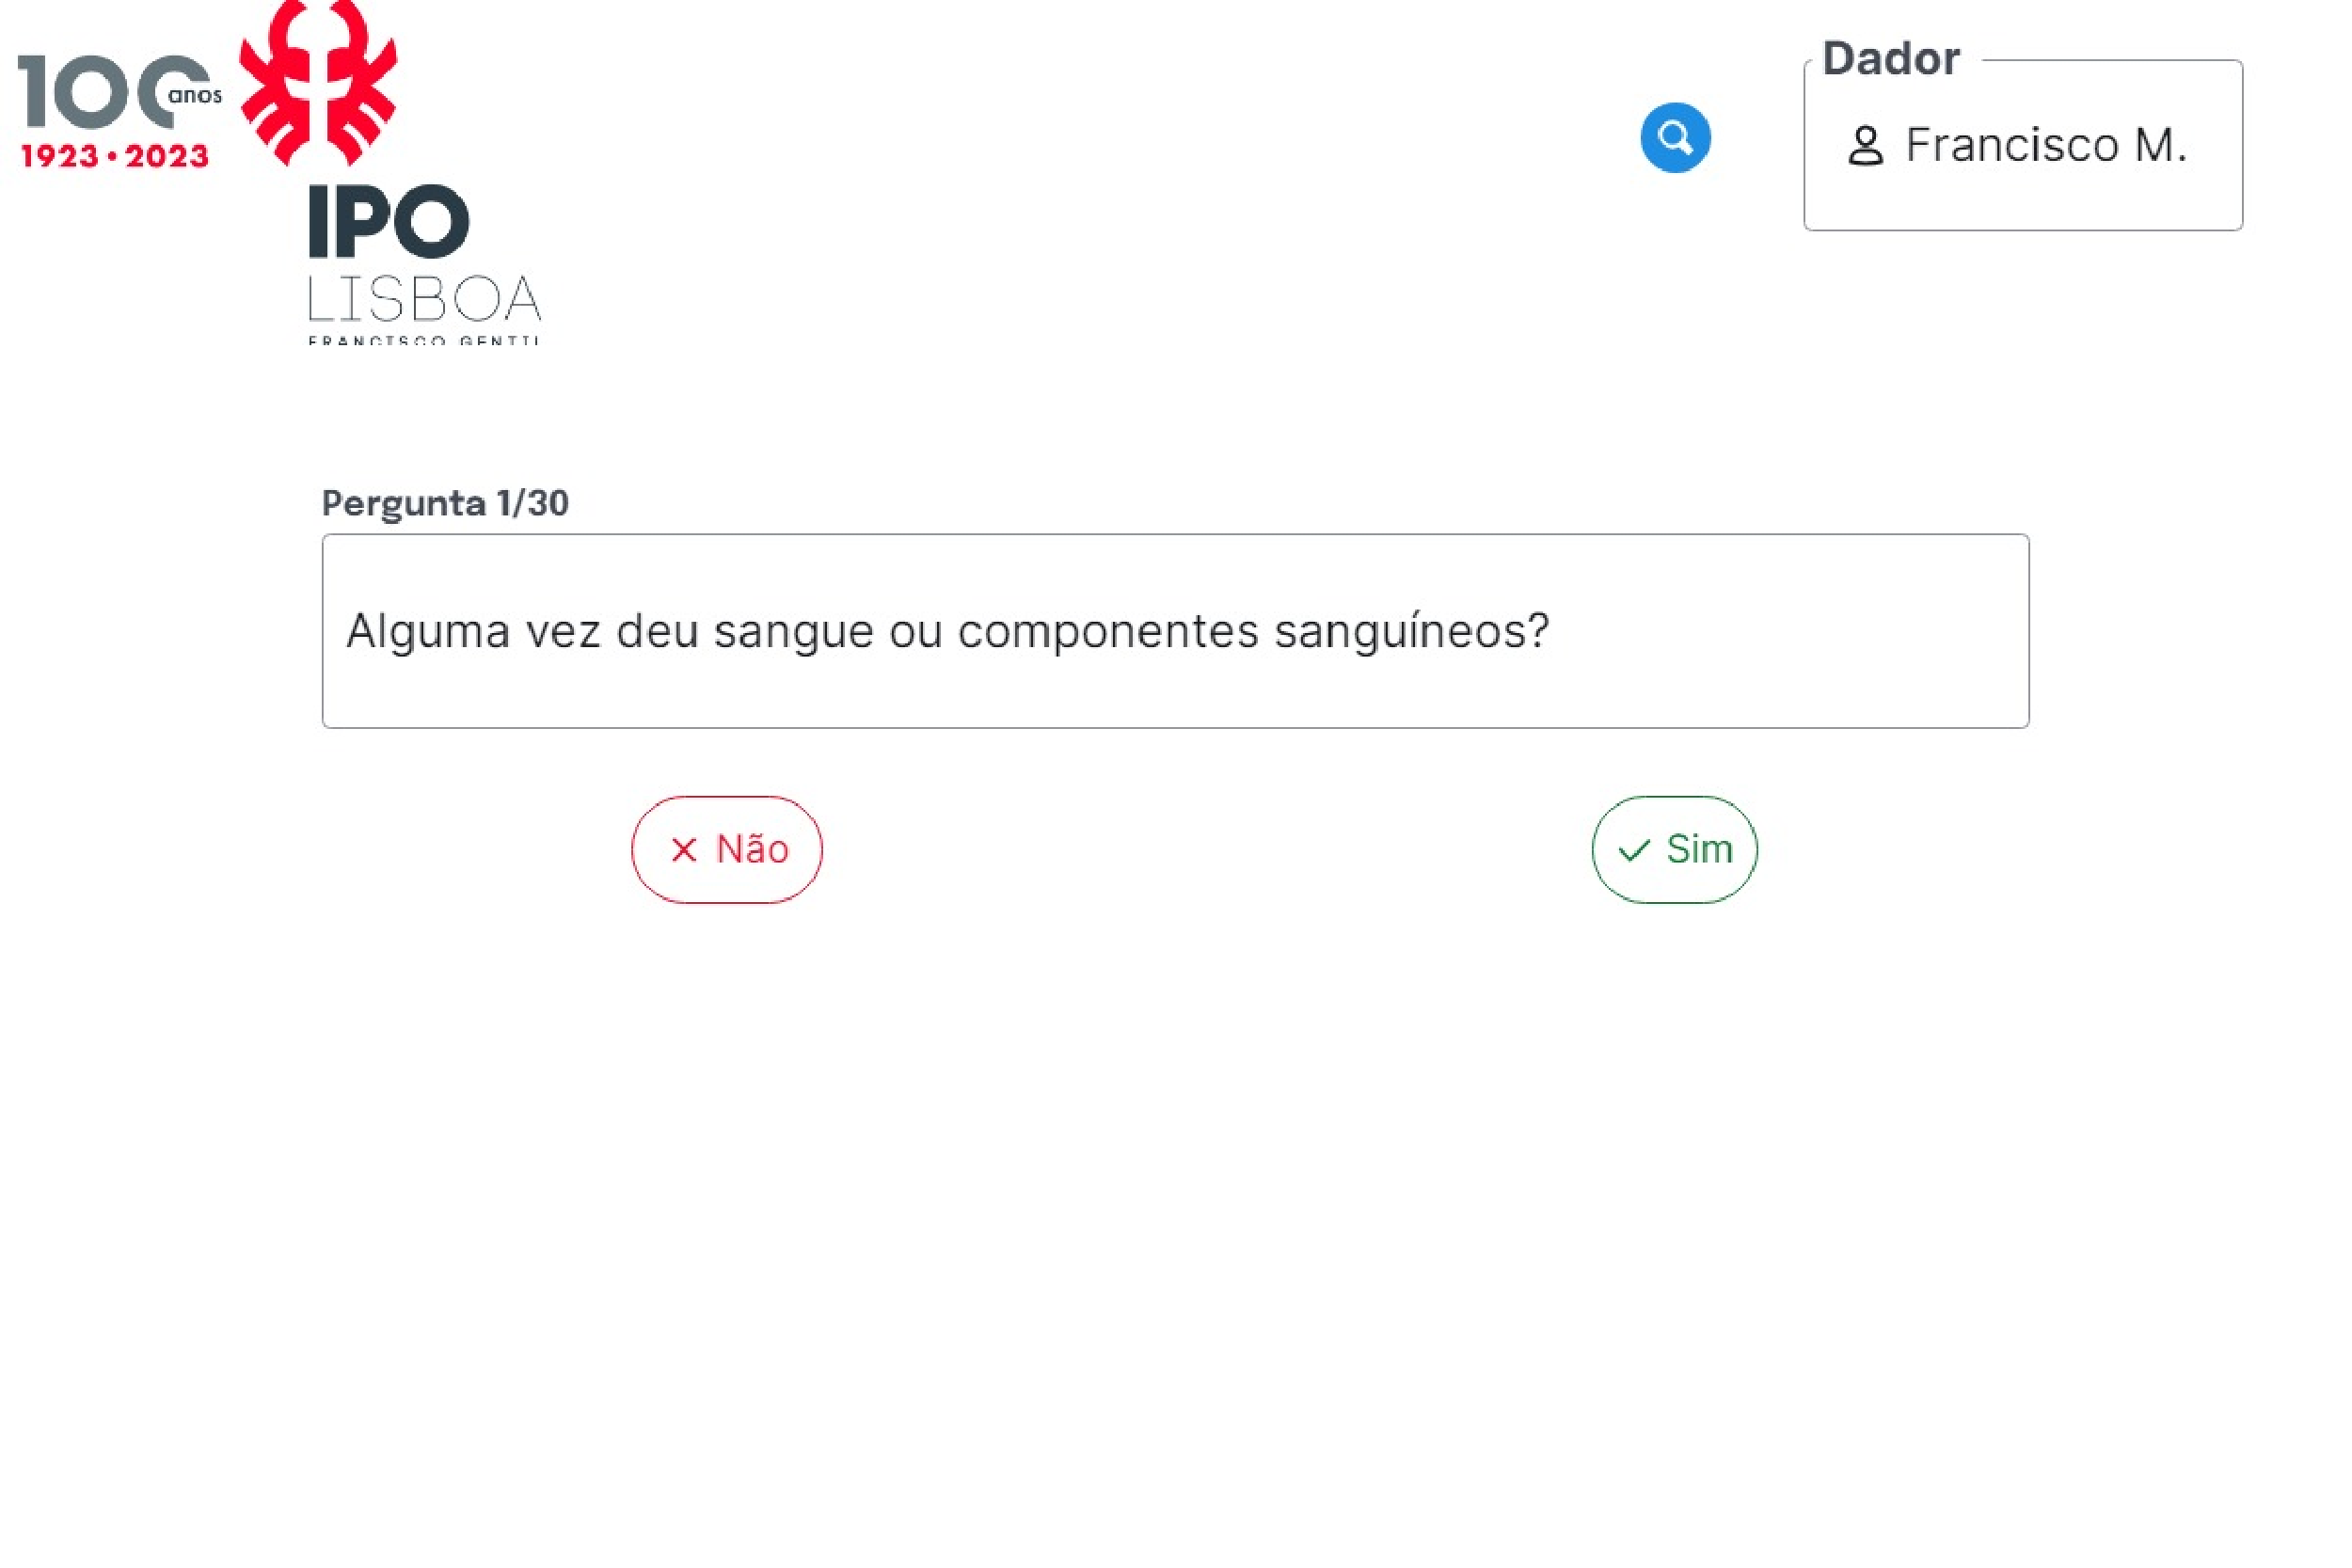
\includegraphics{./figures/Form.pdf}}
	\end{center}
	\caption{Form Page Mock.}\label{fig:form}
\end{figure}

\begin{figure}[h]
	\begin{center}
		\resizebox{160mm}{!}{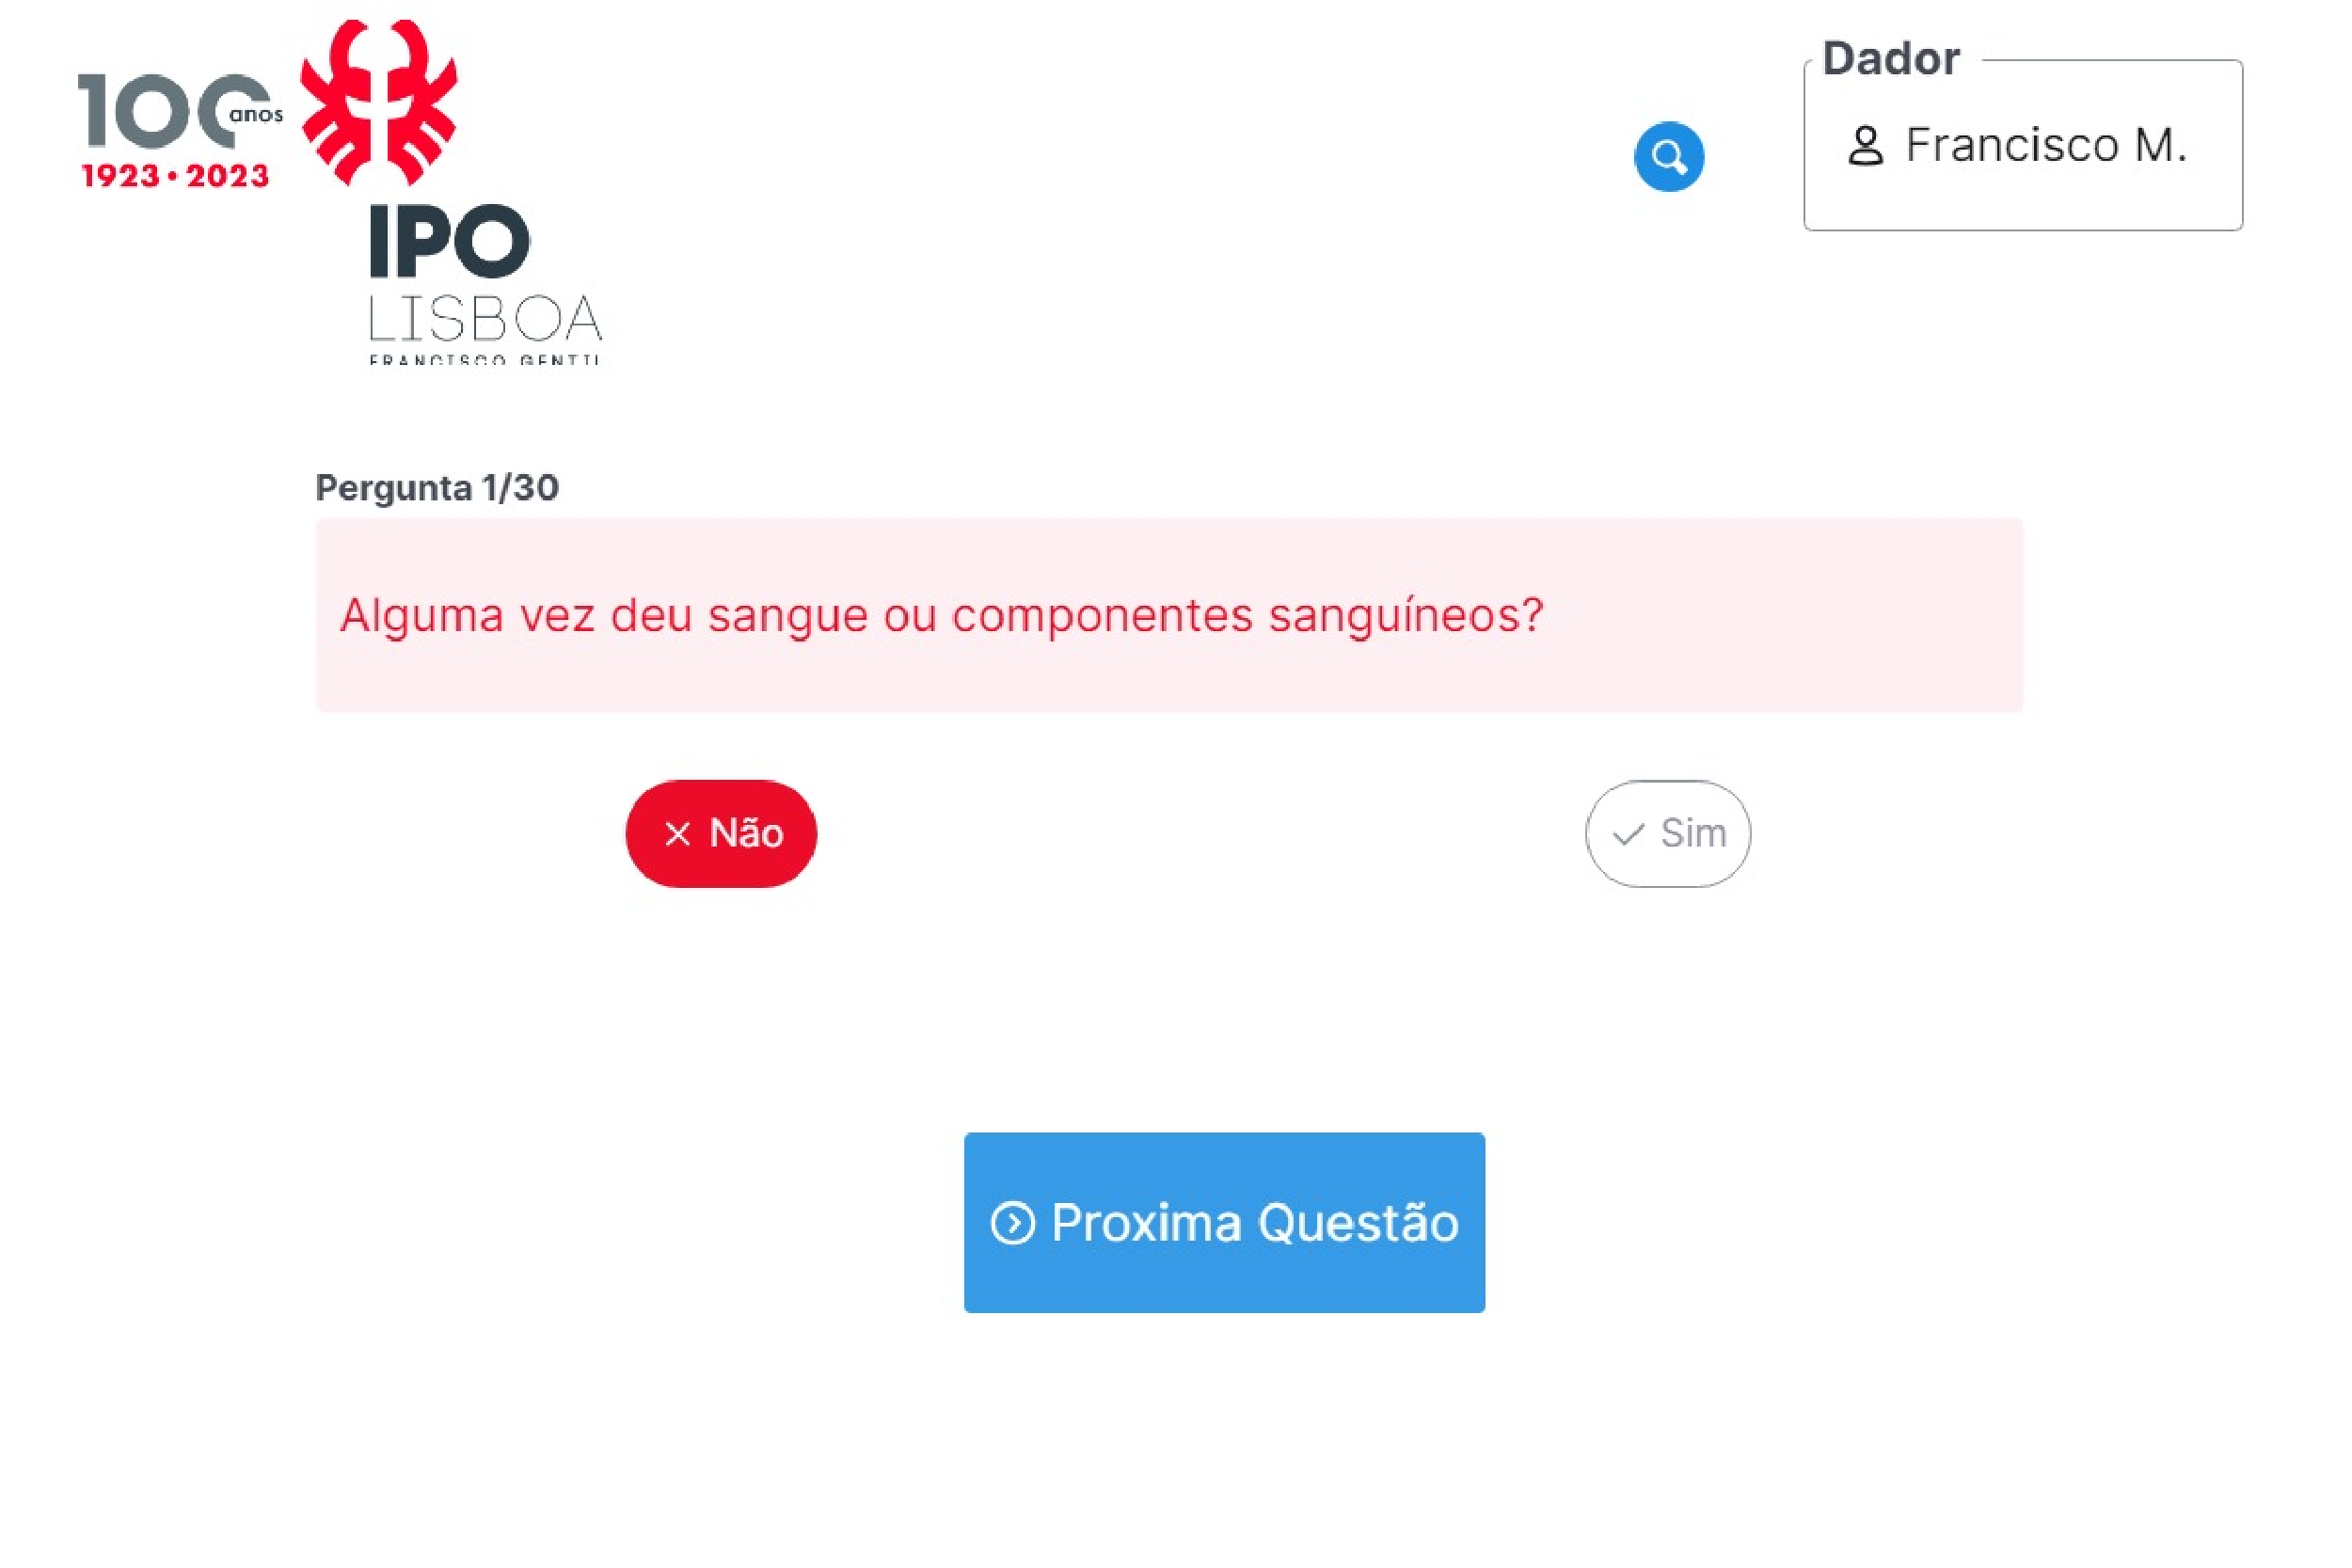
\includegraphics{./figures/Form_Answer_No.pdf}}
	\end{center}
	\caption{Form Page Negative Answer Mock.}\label{fig:form_no}
\end{figure}

\begin{figure}[h]
	\begin{center}
		\resizebox{160mm}{!}{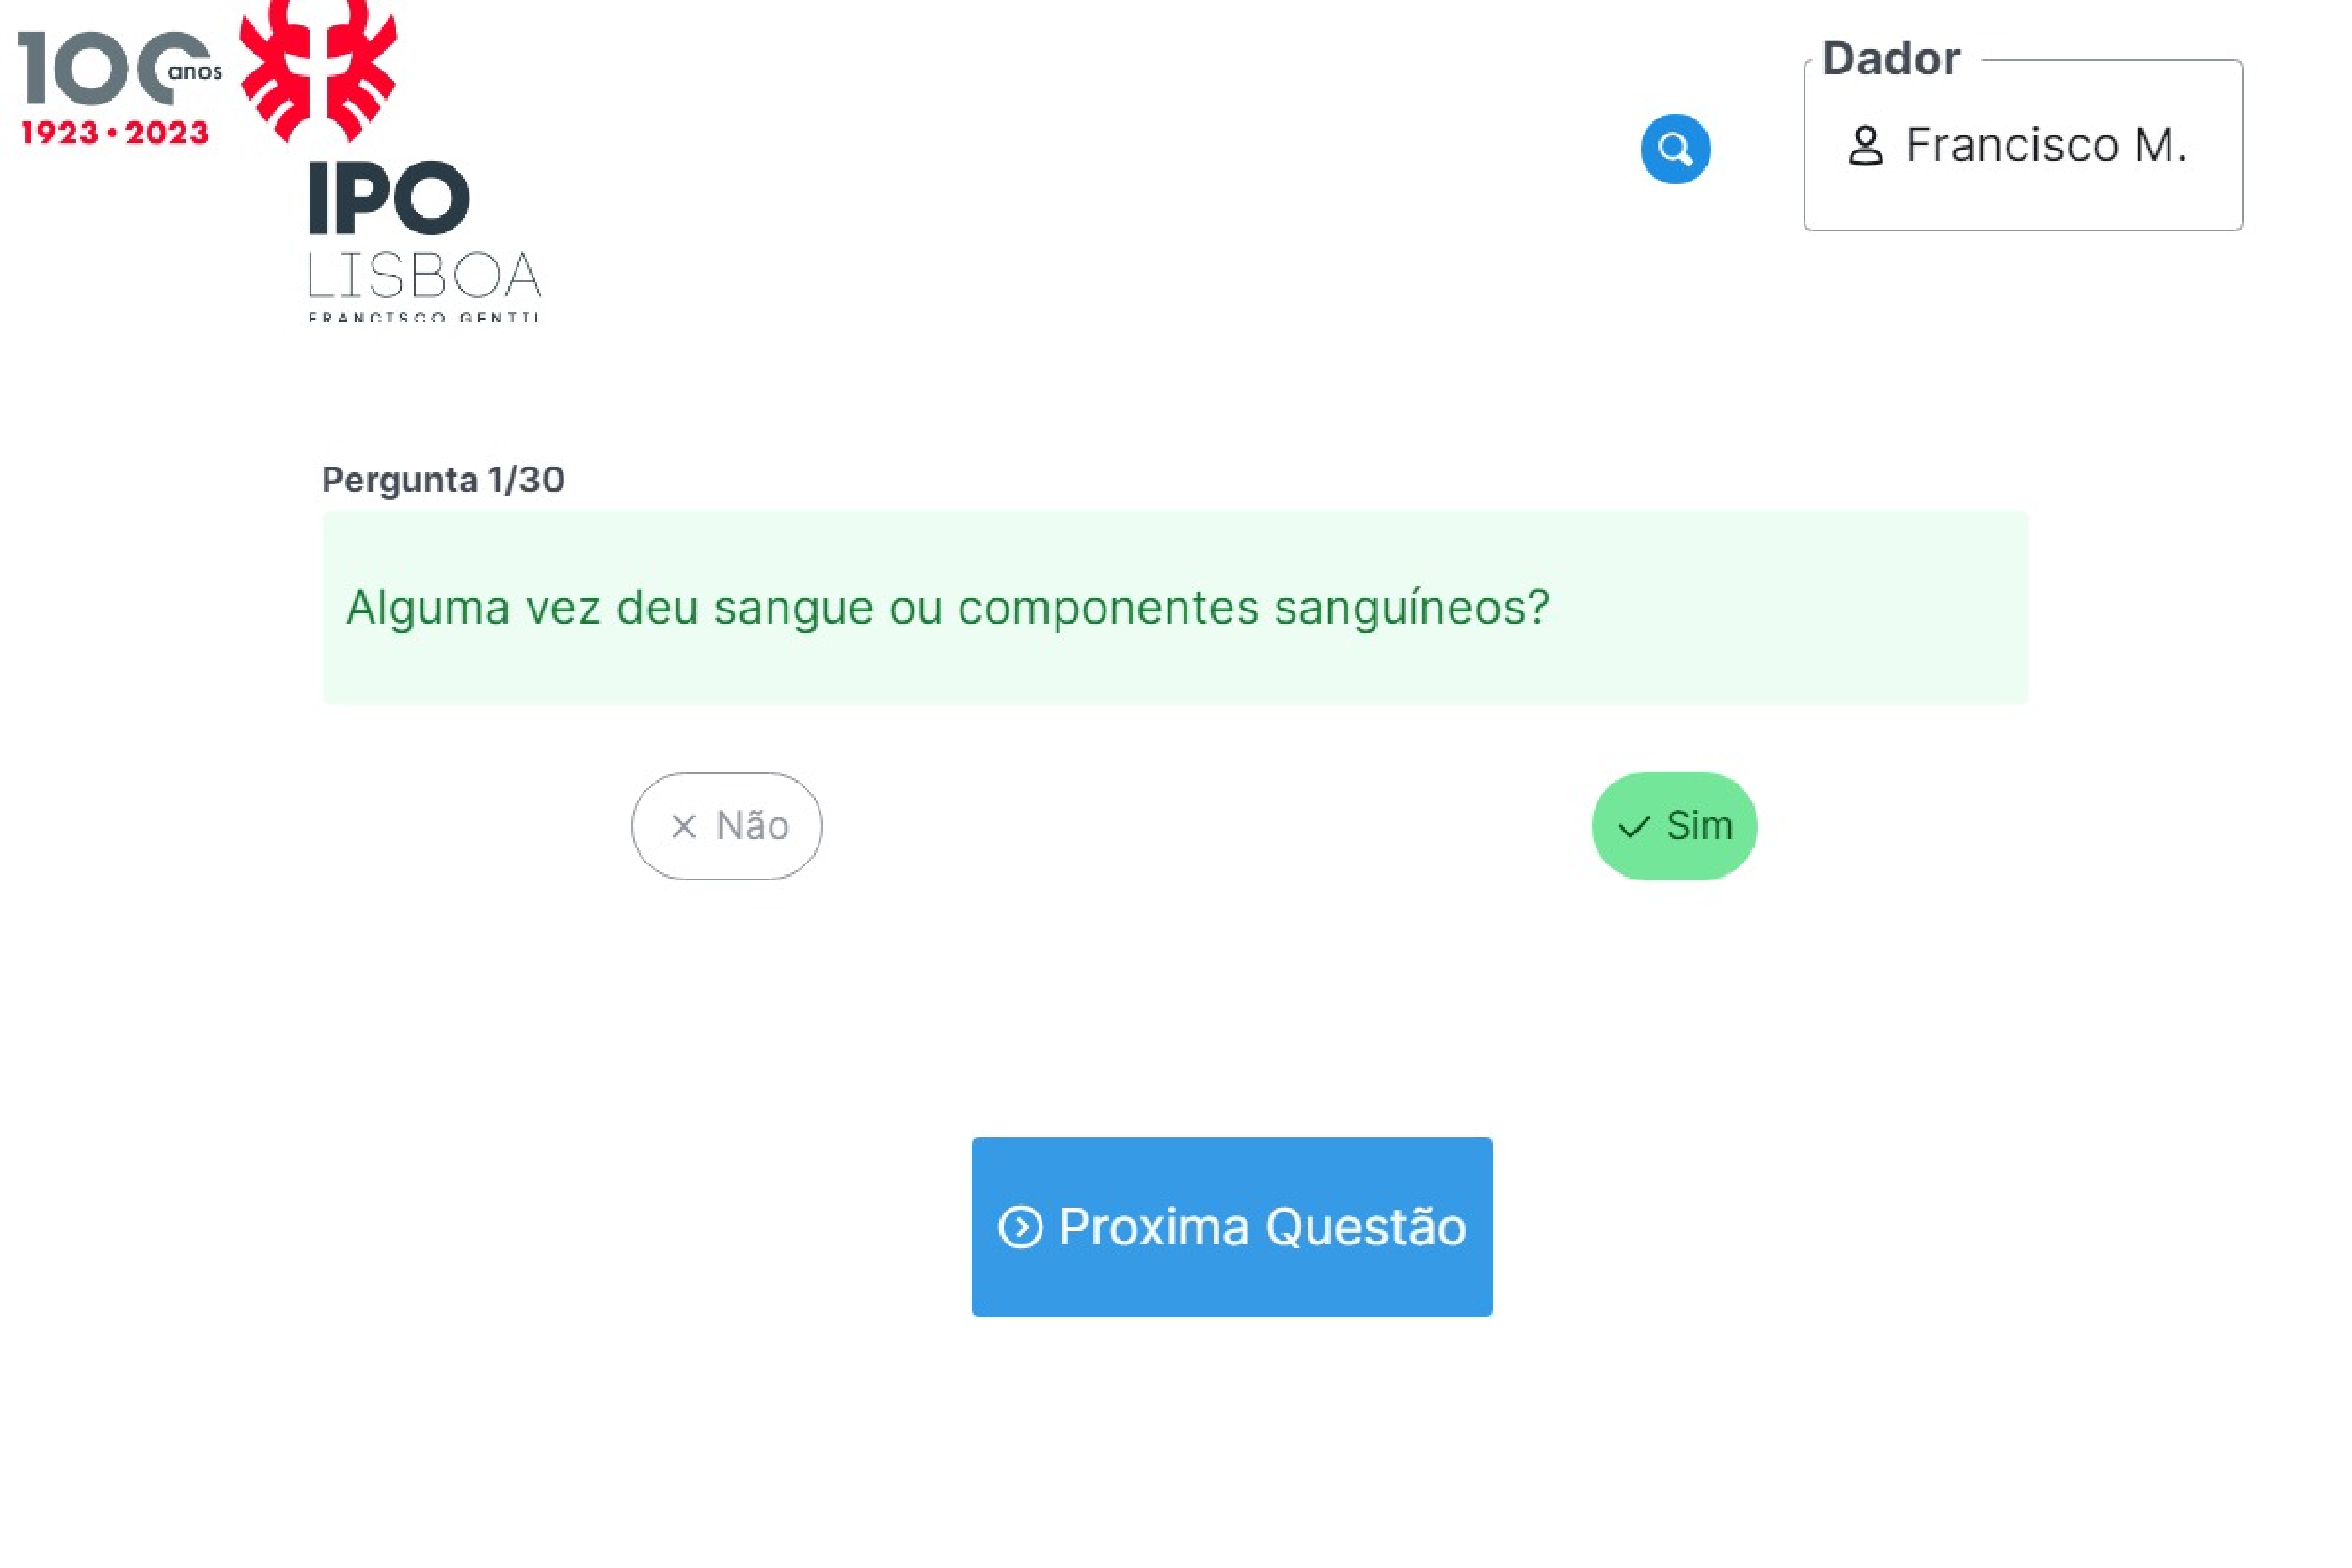
\includegraphics{./figures/Form_Answer_Yes.pdf}}
	\end{center}
	\caption{Form Page Positive Answer Mock.}\label{fig:form_yes}
\end{figure}

\begin{figure}[h]
	\begin{center}
		\resizebox{160mm}{!}{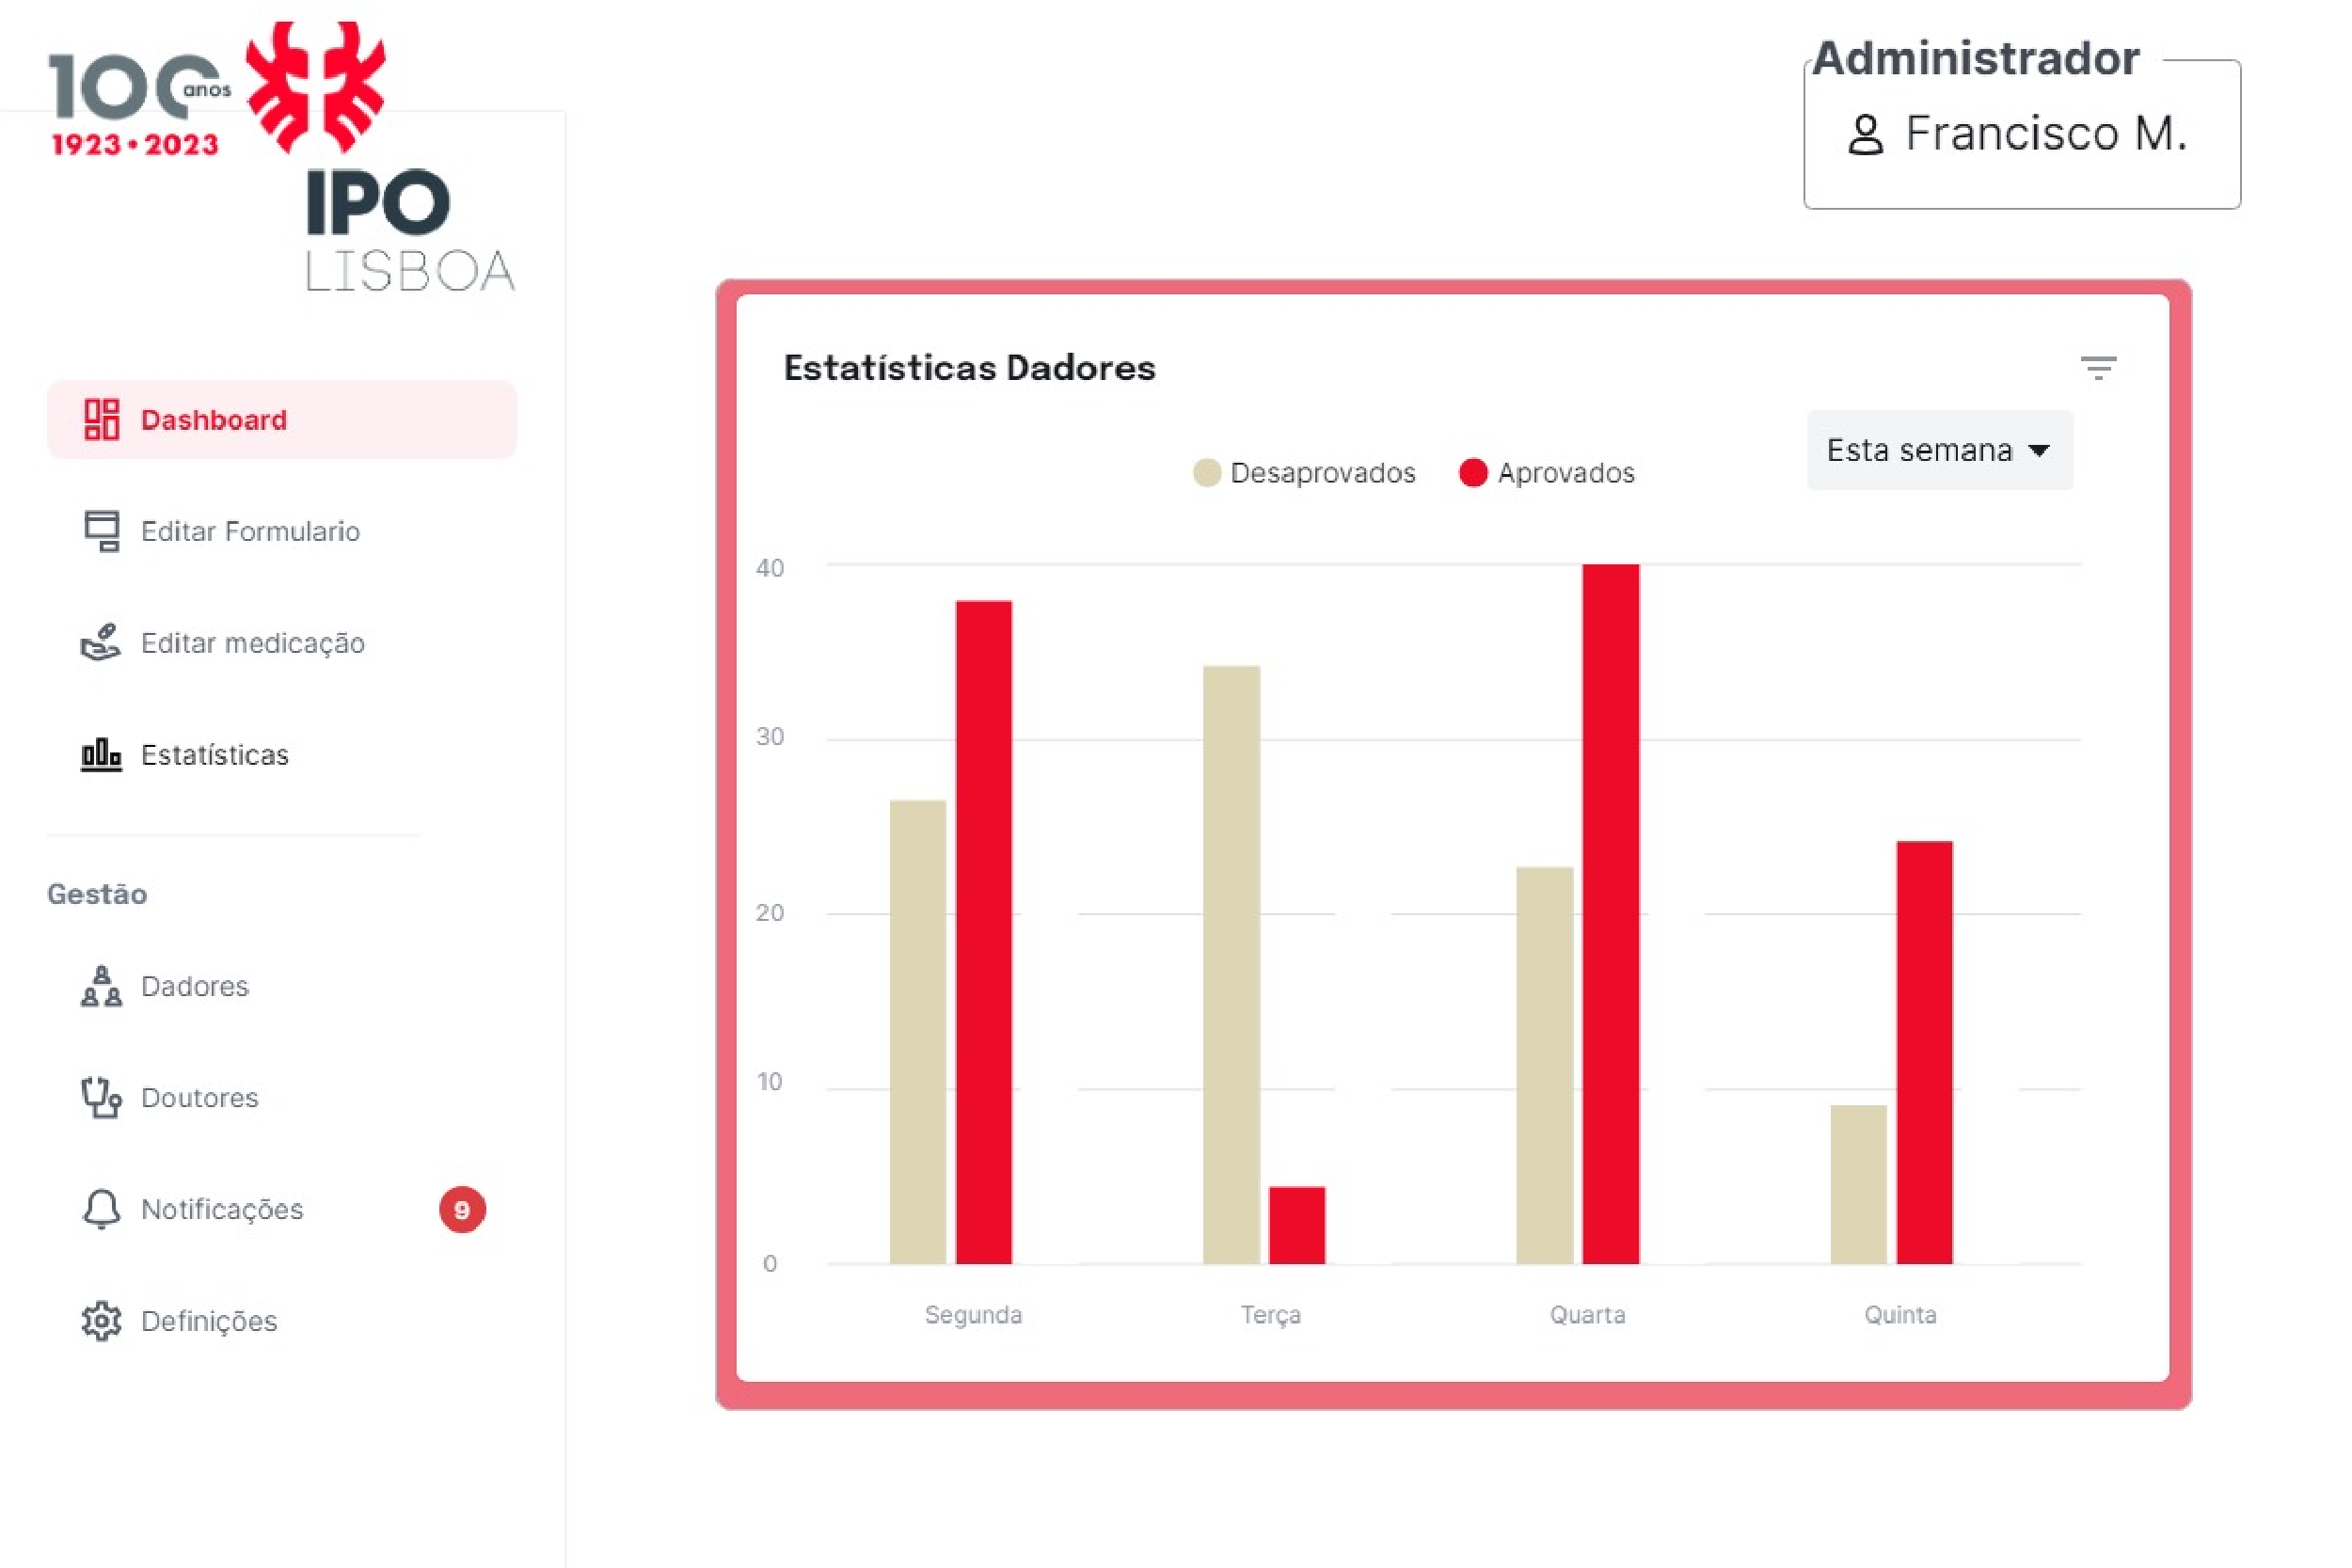
\includegraphics{./figures/Backoffice.pdf}}
	\end{center}
	\caption{Backoffice Page Mock.}\label{fig:backoffice}
\end{figure}




\chapter{Example JSON Form}\label{Form_JSON}


\begin{lstlisting}[style=sharpc]
{
	"language": "en",
	"groups": [
	{
		"name": "Previous Donations",
		"questions": [
		{
			"id": "1",
			"text": "Are you healthy and able to donate blood?",
			"type": "boolean"
		},
		{
			"id": "2",
			"text": "Have you ever donated blood or blood components?",
			"type": "boolean"
		},
		{
			"id": "3",
			"text": "Did you donate blood less than 2 months ago?",
			"type": "boolean"
		}
		]
	},
	{
		"name": "Travel",
		"questions": [
		{
			"id": "4",
			"text": "Have you ever traveled outside the country?",
			"type": "boolean"
		}
		]
	},
	{
		"name": "Health",
		"questions": [
		{
			"id": "5",
			"text": "Have you had any major illnesses or accidents?",
			"type": "boolean"
		}
		]
	},
	{
		"name": "Risk Behaviors",
		"questions": [
		{
			"id": "6",
			"text": "Have you had sexual contact with a new partner in the last 3 months?",
			"type": "boolean"
		}
		]
	}
	],
	"rules": [
	{
		"conditions": {
			"all": [
			{
				"fact": "2",
				"operator": "equal",
				"value": "yes"
			}
			]
		},
		"event": {
			"type": "showQuestion",
			"params": {
				"id": "3"
			}
		}
	},
	{
		"conditions": {
			"all": [
			{
				"fact": "4",
				"operator": "equal",
				"value": "yes"
			}
			]
		},
		"event": {
			"type": "showQuestion",
			"params": {
				"id": "5"
			}
		}
	}
	]
}

\end{lstlisting}

\chapter{User Interface Pages}\label{UI}


\begin{figure}[h]
	\begin{center}
		\resizebox{160mm}{!}{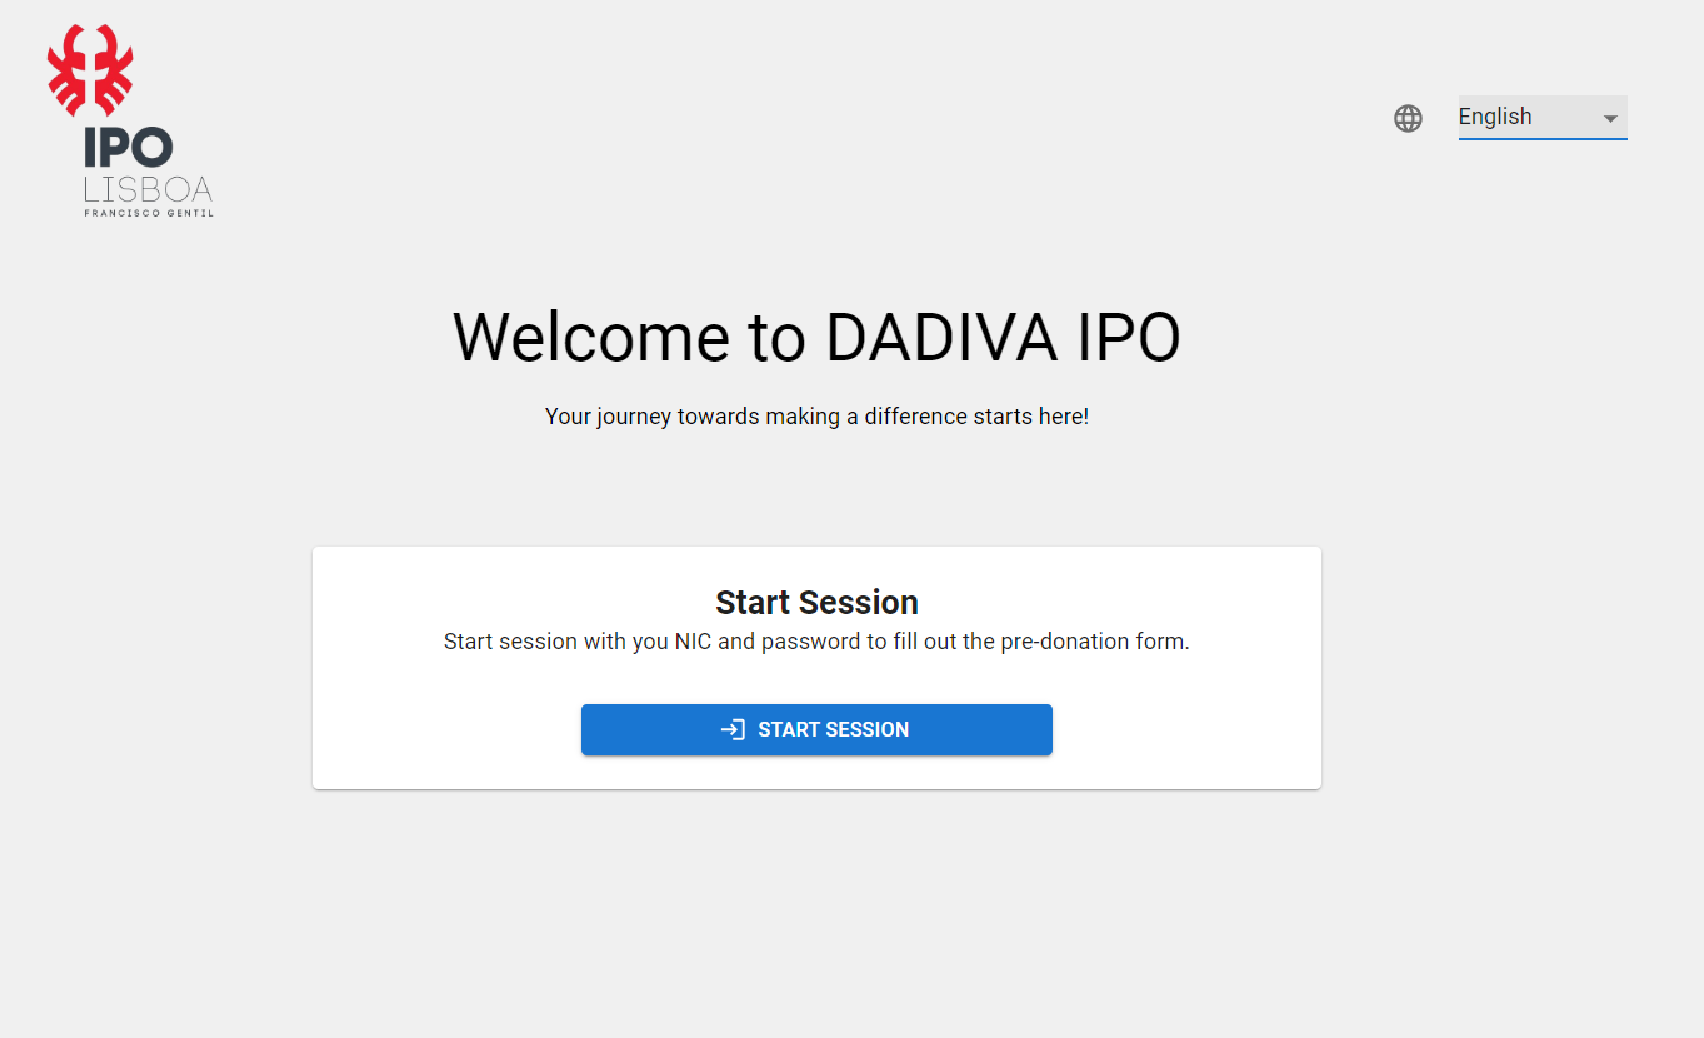
\includegraphics{./figures/Views/Home.pdf}}
	\end{center}
	\caption{Home Page.}
\end{figure}

\begin{figure}[h]
	\begin{center}
		\resizebox{160mm}{!}{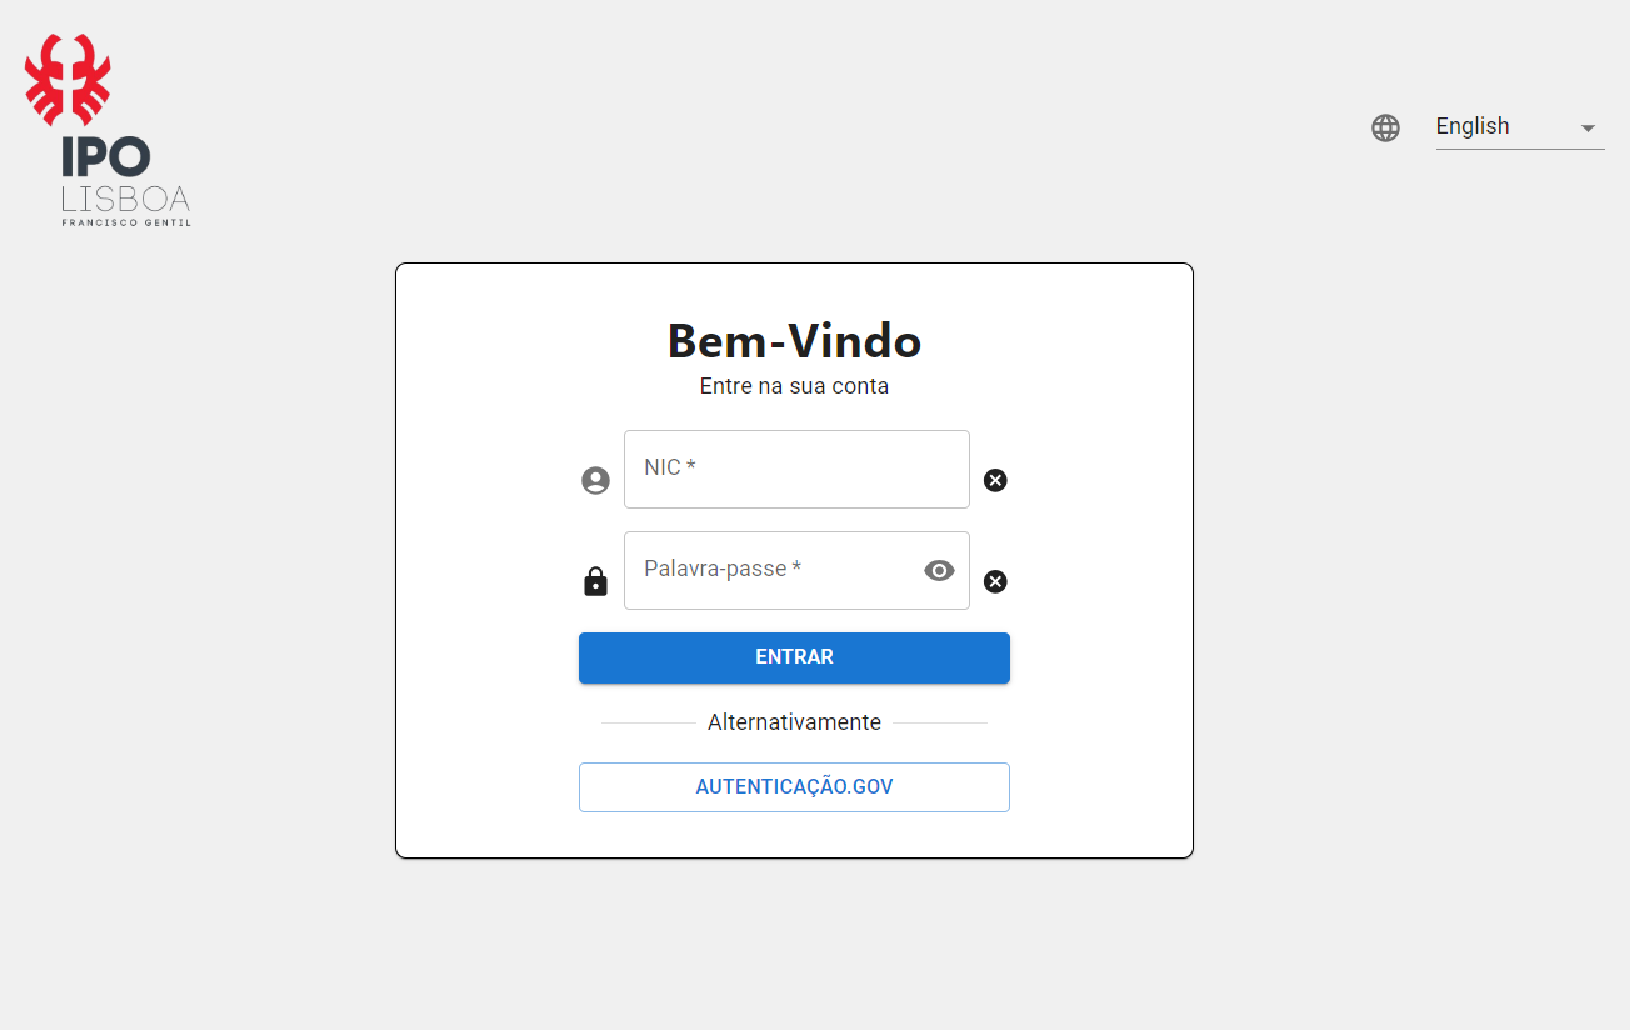
\includegraphics{./figures/Views/Login.pdf}}
	\end{center}
	\caption{Login Page.}
\end{figure}

\begin{figure}[h]
	\begin{center}
		\resizebox{160mm}{!}{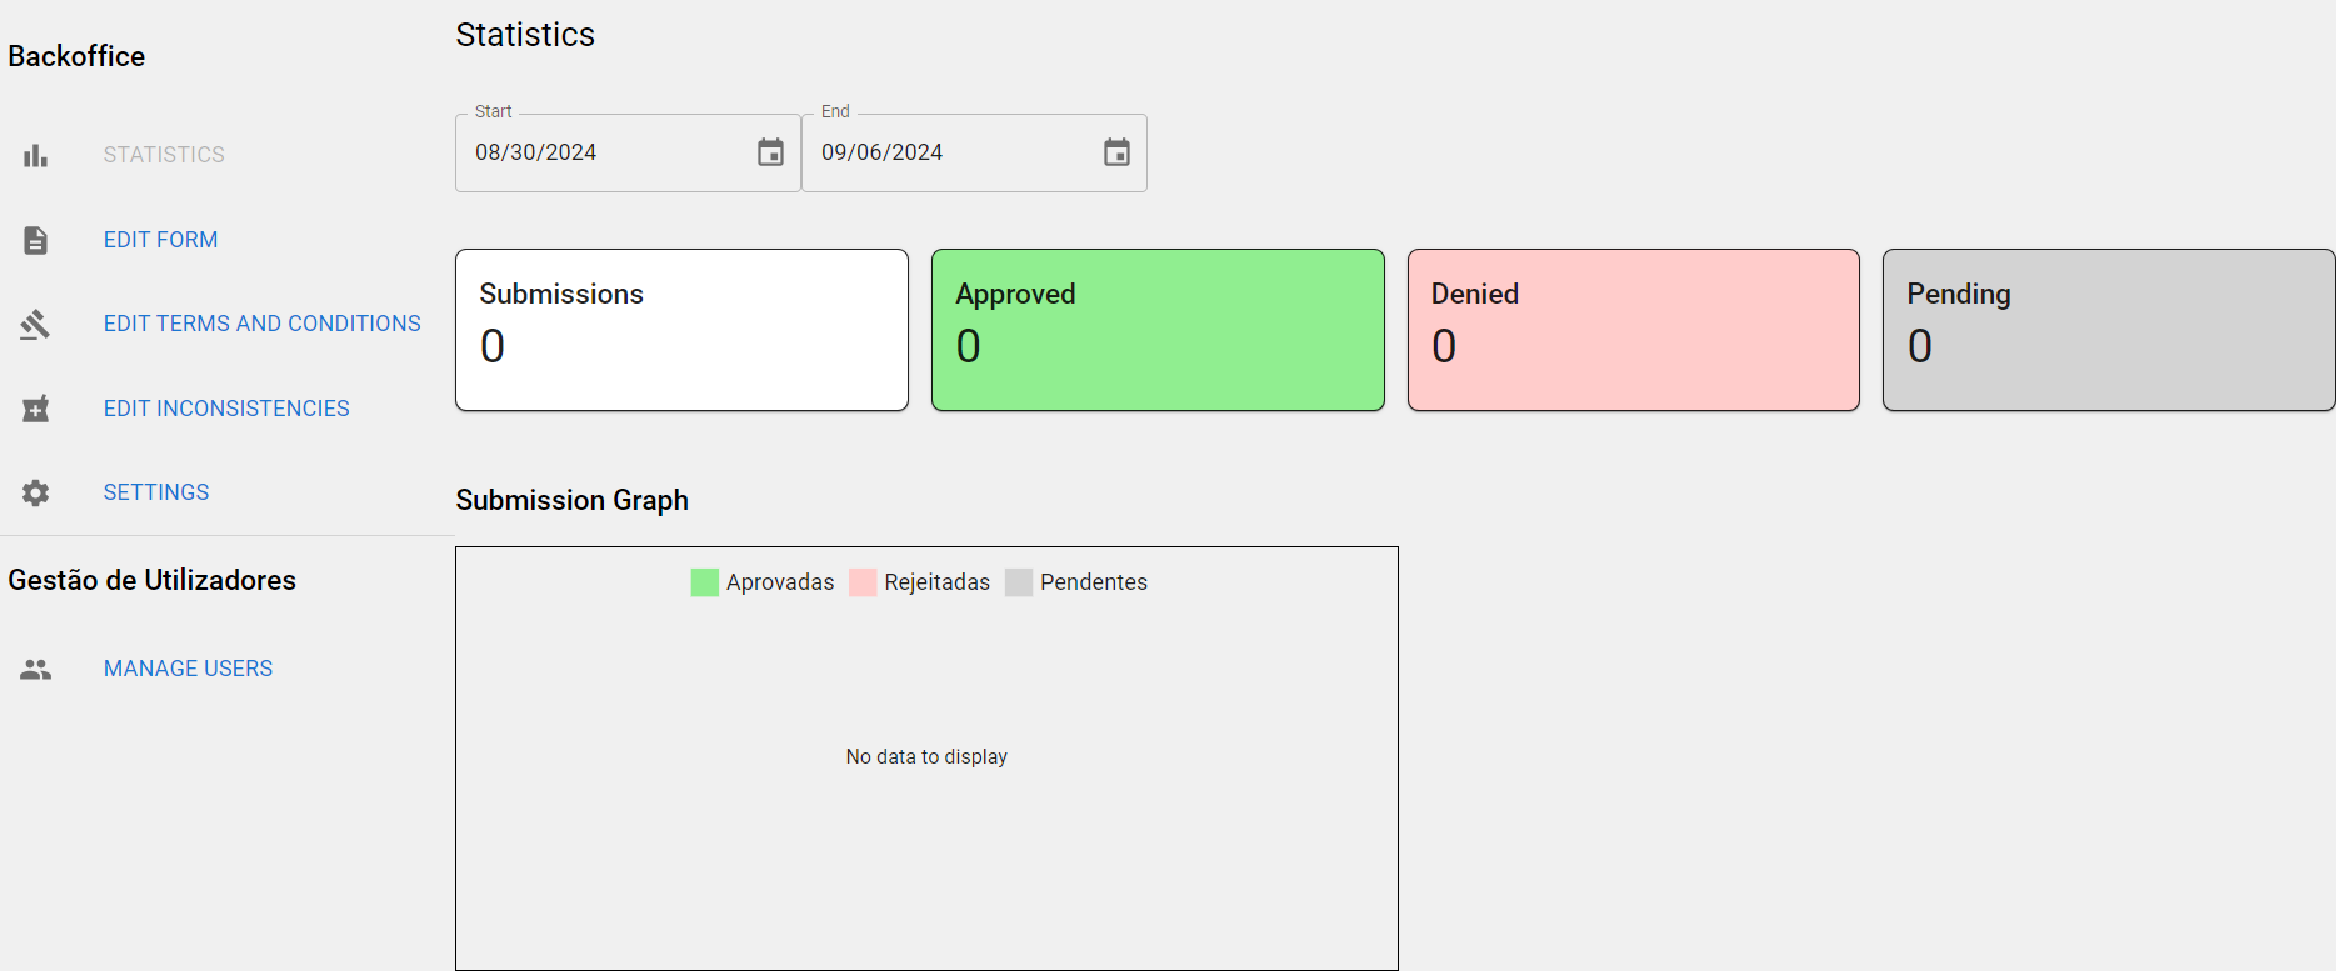
\includegraphics{./figures/Views/Backoffice.pdf}}
	\end{center}
	\caption{Backoffice Page.}
\end{figure}

\begin{figure}[h]
	\begin{center}
		\resizebox{160mm}{!}{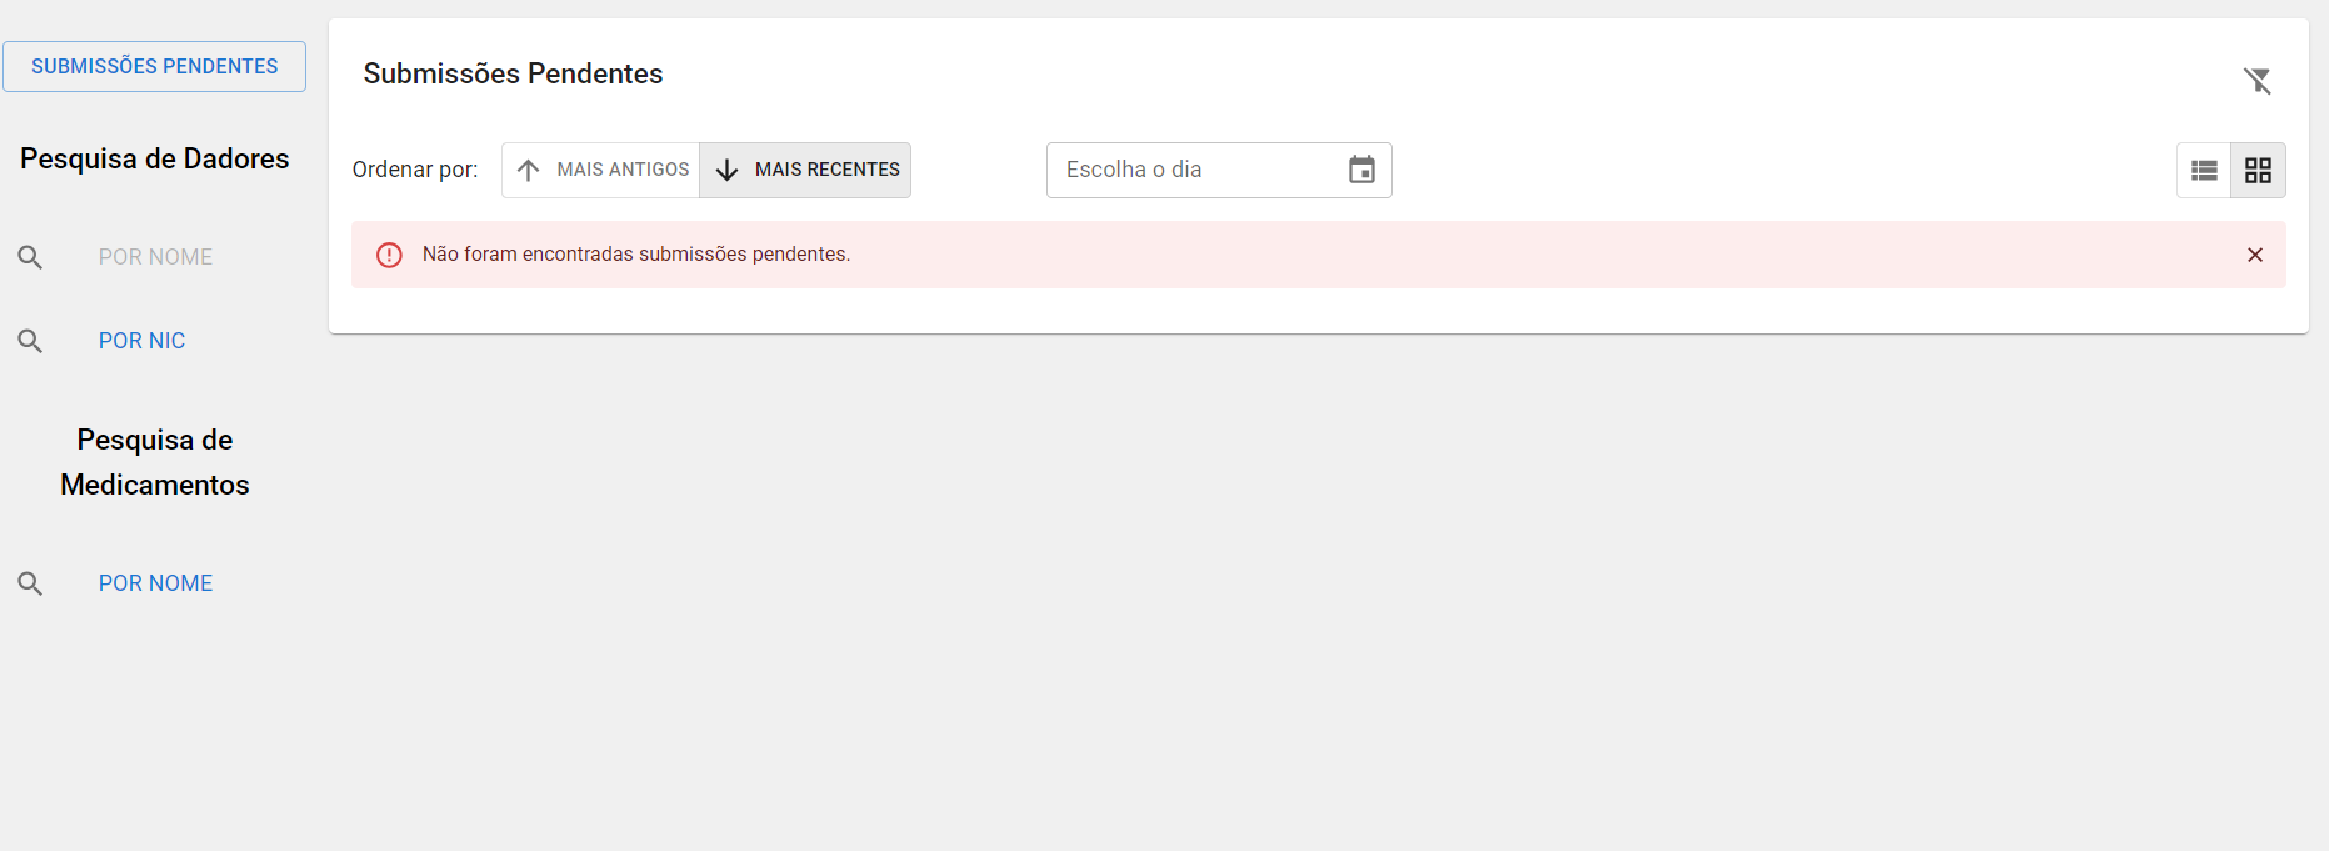
\includegraphics{./figures/Views/Doctor_Page.pdf}}
	\end{center}
	\caption{Doctor Page.}
\end{figure}

\begin{figure}[h]
	\begin{center}
		\resizebox{160mm}{!}{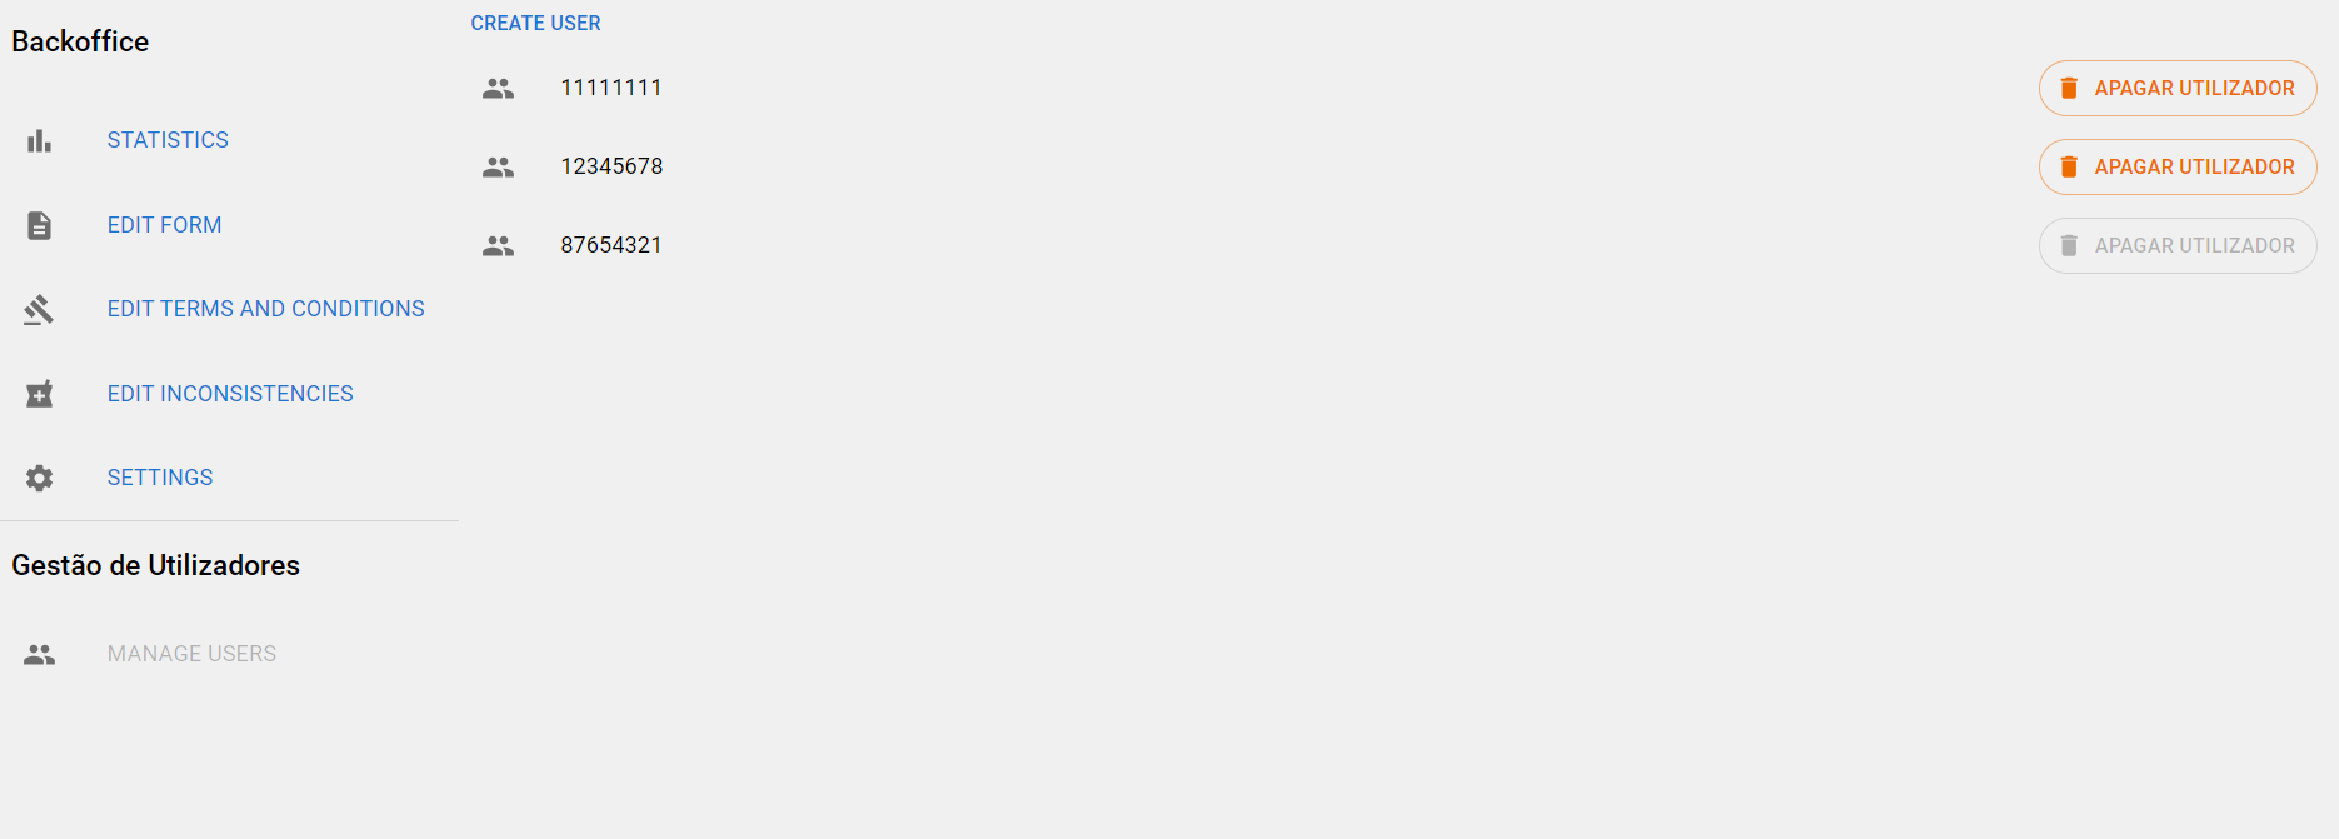
\includegraphics{./figures/Views/Manage_Users.pdf}}
	\end{center}
	\caption{Manage Users Page.}
\end{figure}

\begin{figure}[h]
	\begin{center}
		\resizebox{160mm}{!}{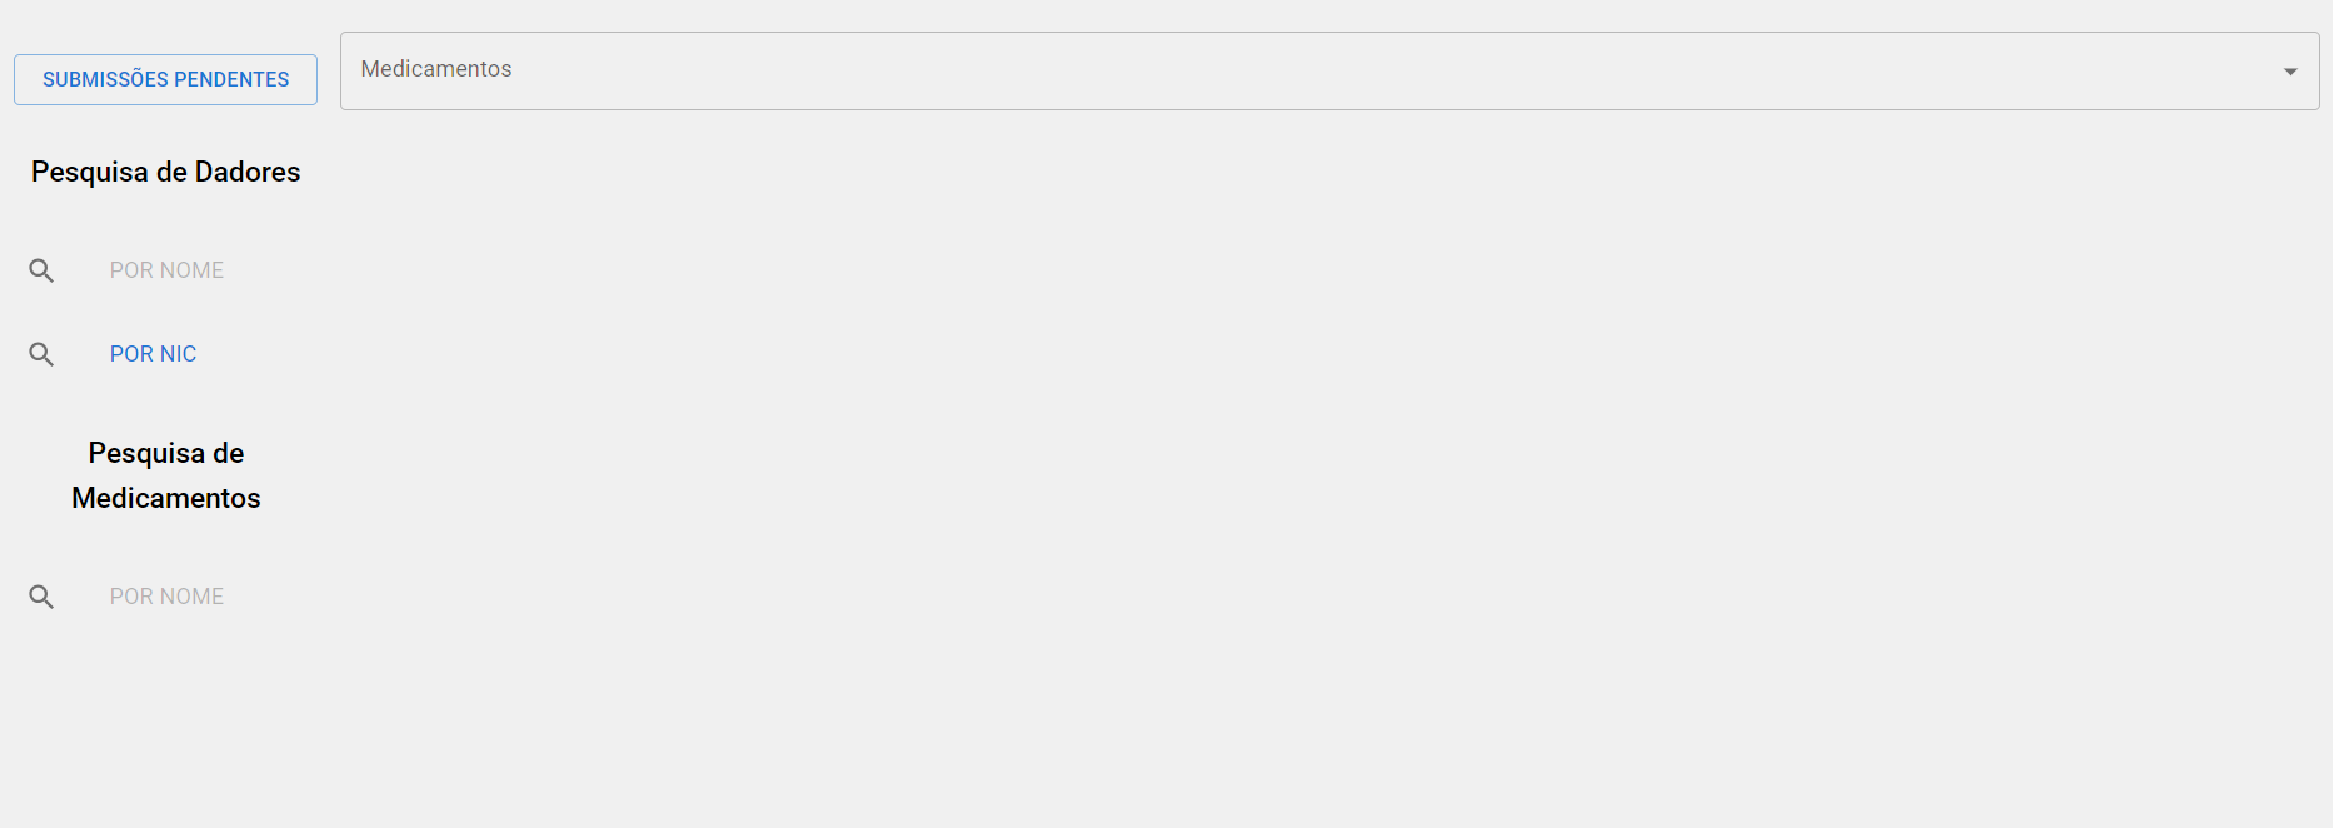
\includegraphics{./figures/Views/Medication_Search.pdf}}
	\end{center}
	\caption{Medication Search Page.}
\end{figure}

\begin{figure}[h]
	\begin{center}
		\resizebox{160mm}{!}{\includegraphics{./figures/Views/User_Terms.pdf}}
	\end{center}
	\caption{User Terms Page.}
\end{figure}

\end{document} 